\documentclass[12pt,twoside,a4paper,openright]{report}
\usepackage{qutthesis}
\usepackage{amsmath}
\usepackage{amssymb}
%\usepackage{amsart}
\usepackage{verbatim}
\usepackage{nomencl}
\usepackage{longtable}
\usepackage{hyperref}
% \usepackage{graphicx}
\usepackage[sort&compress,square]{natbib}
\usepackage{subcaption}
\usepackage{booktabs}
\usepackage{natbib}
\usepackage{multirow}
\usepackage{hhline}
\usepackage{float}
\usepackage{array}
\usepackage{epstopdf}
\usepackage[figuresright]{rotating}
\usepackage{slashbox}
\usepackage[graphicx]{realboxes}
\usepackage[ruled,vlined]{algorithm2e}
\usepackage{color}
\usepackage{float}
\usepackage[final]{pdfpages}
\bibpunct{[}{]}{,}{a}{,}{,}
%\usepackage{named}

% correct bad hyphenation here
\hyphenation{op-tical net-works semi-conduc-tor}


%%%%%%%%%%%%%%%%
\begin{document}

%%%%%%%%%% Front Part: Cover page, abstract, ack, preface
% Part0FrontPart.tex

%============frontmatter % Coverpage etc
\title{Acoustic classification of Australian frogs for ecosystem surveys}
       
\author{Jie Xie}
%\authoremail{xiej8734@gmail.com}
\supervisor{Dr Jinglan Zhang, Professor Paul Roe, Dr Michael Towsey, Professor Vinold Chandran}
\thesistype{Doctor of Philosophy}    % or comment it out (the default is Doctor of Philosophy)
\university{Queensland University of Technology} % or comment it out (the default is QUT)
\faculty{Science and Engineering Faculty}   % or comment it out (the default one is SEF)
\school{School of Electrical Engineering and Computer Science}   % or School of xxx xxx xxx 
                         % or comment it out (the default one is Elec Eng and Computer Science)                         
%\universitylogo{yes}{1.0}{./QUTLogo.eps}  % yes (true, 1) or no (false, 0), scale = 1.0; filename = QUTLogo.eps

%

\submissiondate{July 2016}
\copyrightyear{2016}
%\informationcutoffdate{01 March 2010} %for cut of date of information in the thesis

\maketitle	   %cover page of the thesis; a blank page is automatically added for double-side printing

%\blankpage         %two more blank pages. If you don't want them, comment them out
% \blankpage

\setcounter{page}{1} %start to count page numbers

% \insidetitlepage   %if you don't like an insidetitle page, comment it out

\copyrightpage     %another format available: \copyrightpageWithTitle. You may try it (with thesis title). 

%\signaturepage\cleardoublepage   % you may not need this signature page, so comment it out

%============dedication
\begin{dedication}
To my family 
\end{dedication}

%============abstract
\begin{abstract}
Rapid decreases in frog populations, which are regarded as one of the most critical threats to global biodiversity, have been spotted from locations around the world. Causes of these declines can be summarised as follows: disease, habitat destruction and modification, exploitation, pollution, pesticide use, introduced species, and ultraviolet-B radiation (UV-B). On the one hand, frogs play an important role in the whole ecosystem, but on the other frog populations are declining globally. To assess frog populations and optimise frog protection policies, monitoring frogs is becoming ever more necessary. Since frogs are much easier to be heard than seen, frog populations are often assessed by their vocalisations. In order to collect frog vocalisations, traditional manual methods require ecologists and volunteers to visit the field, which limits the        
scale for acoustic data collection. In contrast, recent advances in acoustic sensors provide a novel method to survey vocalising animals such as frogs. After deploying acoustic sensors in the field, they can automatically collect acoustic data at large spatial and temporal scales. The large volumes of raw acoustic data collected must be analysed to gain insights about frogs and the environment. It has become very important to enable automated species identification in acoustic data. Also, since the data is collected from the field, the acoustic data tend to be very noisy and very often the desired signal (frog call) is weak. Very often, there are also multiple signals overlapping the frog calls. These characteristics pose a big challenge to performing automatic classification of frog species in acoustic data.



The research presented in this dissertation aims to investigate methods to build a robust and accurate classification prototype system for frog species in acoustic data. Two important aspects of a classification prototype system are investigated: feature extraction and classification, which consist of contributions towards three main objectives.
\begin{enumerate} 
\item[(1)]	Develop an enhanced feature representation for frog call classification (Chapter \ref{cha:cha4EnhancedFeature}). 
\\
Time-frequency information of frog calls can be effectively represented via the enhanced representation of temporal, perceptual and cepstral features. The classification performance of various machine learning techniques is compared with different feature representations. Our proposed enhanced feature representation achieves a satisfied classification accuracy.
 
\item[(2)]	Propose a novel feature representation based on adaptive wavelet packet decomposition (Chapter \ref{cha:cha5WaveletFeature}). 
\\
To better capture the frequency domain information of frog calls with a good anti-noise ability, a novel feature representation, namely \textit{adaptive frequency scaled wavelet packet decomposition sub-band cepstral coefficients}, is proposed. Compared with other cepstral coefficients, the proposed feature representation shows the best classification performance and a good anti-noise ability.

\item[(3)]	Design a robust classification system to study low signal-to-noise ratio (SNR) recordings with multiple simultaneously vocalising frog species. Two classification frameworks are employed to classify multiple simultaneously vocalising frog species. 


\begin{enumerate}
\item Multiple-instance Multiple-label (MIML) learning (Chapter \ref{cha:cha6MIML})
\\
To use MIML learning for classifying multiple simultaneously vocalising frog species, individual syllables are first segmented. Then, various features are calculated from each segmented syllable. Next, a bag generator is applied to those extracted features to construct a suitable bag-of-syllable representation. Finally, three MIML learning algorithms are employed for the classification of frog vocalisations: MIML-SVM, MIML-KNN, and MIML-RBF. 

\item Multiple-label (ML) learning (Chapter \ref{cha:cha7ML})
\\
For the ML learning, acoustic features are first calculated without segmentation. Then, ML learning is used to classify simultaneously vocalising frog species using extracted features. Three main ML learning methods are compared: Binary relevance, Classifier Chains, Random k-labelsets, where the base classifier is a decision tree classifier. Furthermore, the frog abundance and species richness over three months are estimated based on the results of acoustic event detection and ML classification, respectively. 
Lastly, the correlation analysis between frog calling activity (frog abundance and species richness) and weather variables (mean temperature and rainfall) are studied to demonstrate the application of our proposed ML classification framework.
\end{enumerate}


\end{enumerate} 


Our proposed approach achieves promising classification results compared with most previous studies. Novel feature representations and classification learning frameworks have different contributions to the performance of the classification system of frog vocalisations. To cope with high SNR recordings, we construct a novel feature representation including temporal, perceptual, and cepstral features. To improve the anti-noise ability of cepstral features, we develop a novel wavelet-based ceptral feature representation. To address low SNR recordings with multiple overlapping vocalising frog species, the classification frameworks of MIML learning and ML learning are proposed. To the best of this researcher's knowledge, it is the first time that MIML learning and ML learning are employed for automatic classification of multiple simultaneously vocalising frog species.
With this developed classification system, the ecosystem at large spatial and temporal scales can be surveyed, which can help ecologists better understand the ecosystem. 


\end{abstract}



%\newpage
%\begin{center}
%{\huge \textbf{List of Abbreviations}}
%\end{center}
%
%\begin{table}[htb!]
%%\caption{My caption}
%%\label{my-label}
%\begin{tabular}{lllll}
%DFT   &  &  &  & Discrete Fourier Transform          \\
%DCT   &  &  &  & Discrete Cosine Transform           \\
%SNR   &  &  &  & Signal to Noise Ratio               \\
%LPCs  &  &  &  & Linear Predictive Coding            \\
%MFCCs &  &  &  & Mel-Frequency Cepstral Coefficients \\
%LDA   &  &  &  & Linear Discriminant Analysis        \\
%K-NN  &  &  &  & K-Nearest Neighbour                 \\
%SVM   &  &  &  & Support Vector Machine              \\
%ANN   &  &  &  & Artificial Neural Network           \\
%RF    &  &  &  & Random Forest                       \\
%AED   &  &  &  & Acoustic Event Detection            \\
%WPD   &  &  &  & Wavelet Packet Decomposition        \\
%MIML  &  &  &  & Multiple-Instance Multiple-Label    \\
%ML    &  &  &  & Multiple Label                     
%\end{tabular}
%\end{table}



%============keywords
\begin{keywords}
Bioacoustic monitoring \\
Soundscape ecology\\
Environmental audio analysis \\
Frog call classification \\
Spectrogram analysis \\
Acoustic feature extraction \\
Wavelet packet decomposition \\
Multiple-instance multiple-label learning \\
Multiple-label learning \\
 
\end{keywords}






%============acknowledgement
\begin{ack}
First, I would like to express my sincere gratitude and thanks to Dr Jinglan Zhang (principal supervisor), for giving me an opportunity to study in Australia. During the entirety of this PhD study, I have learnt so much from her about having passion for work, combined with high motivation, which will benefit me throughout my life. 
I would also like to express my gratitude to Professor Paul Roe (associate supervisor), for his consistent instructions and supports through the last three years.  

I would also like to thank Dr Michael Towsey for his provision of consistent guidance, discussions, and encouragement during my PhD study. Michael's attitude towards scientific research keeps motivating me go deeper into research.  


I want to thank Professor Vinod Chandran for his support in writing my confirmation report and this thesis. Vinod's strong background knowledge in signal processing greatly helps me improve my understanding of this research.

I would also like to express my gratitude to my family, especially my grandparents, parents and my wife. They have always supported my overseas study. Without their support, I could not give my full attention to PhD study and  the completion of this thesis. 
My sincere thanks also go to all my friends for their love, attention and support to my PhD study. 

Finally, I extend my thanks to the China Scholarship Council (CSC), Queensland University of Technology and the Wet Tropics Management Authority for their financial support. 

\end{ack}


%=============preface
%\begin{preface}
%%Here is the preface. 
%%
%\end{preface}


%==============
% If you don't like to put nomenclature, which you have manually 
% edited in the file nomenclature.tex, at the front, comment the 
% following line out
% \listnomenclatureatfront{yes}{./nomenclature.tex} 

%==============
\afterpreface
           %Ch0FrontPart.tex
                                   %   including title page information, abstract,
                                   %   acknowledgement, etc
%%% Body Text
% nomenclature

%\newenvironment{nomenc}{\prefacesection{Nomenclature}}{}

\chapter*{List of Abbreviations}

\addcontentsline{toc}{chapter}{Abbreviations}
\pagenumbering{gobble}

\renewcommand{\arraystretch}{1.4} 
\begin{longtable}{llr}
\multicolumn{3}{l}{\textbf{}\hspace{0.4\textwidth}~~}\\
\textbf{DFT}   &                    Discrete Fourier Transform \\
\textbf{DCT}    &                    Discrete Cosine Transform \\
\textbf{STFT} & Short-Time Fourier Transform \\
\textbf{LPCs}	 &                   Linear Predictive Coding \\
\textbf{MFCCs} &	       Mel-Frequency Cepstral Coefficients \\
\textbf{LDA}      &                  Linear Discriminant Analysis \\
\textbf{K-NN}	  &                  K-Nearest Neighbour \\
\textbf{SVM}	     &               Support Vector Machine \\
\textbf{ANN}    &                   Artificial Neural Network \\
\textbf{RF}     &                      Random Forest \\
\textbf{AED}	   &                 Acoustic Event Detection \\
\textbf{WPD}     &                 Wavelet Packet Decomposition \\
\textbf{MIML}   &                 Multiple-Instance Multiple-Label  \\ 
\textbf{ML}    &                      Multiple-Label \\
\end{longtable}


% Ch1Introduction.tex

\chapter[Introduction]{Introduction}
\label{cha:cha1Introduction}

%=============
\section{Motivation and background}
During the past decades, rapid decreases in frog populations have been spotted from locations over the world, which are regarded as one of the most critical threats to the global biodiversity. Many environment problems are regarded as the reasons for these declines: disease, habitat destruction and modification, exploitation, pollution, pesticide use, introduced species, and ultraviolet-B radiation (UV-B). 
On one hand frog populations are rapidly worldwide declining, and on the other frogs are greatly important to the global ecosystem. 
\begin{enumerate}
\item[(1)] Frogs are integral part of the food web
\item[(2)] Frogs are often used as the environment indicators 
\item[(3)] Frogs are important in medical research that benefits humans 
\end{enumerate}

For those aforementioned reasons, increasing frog populations and optimising the protection policy necessitates monitoring of frogs. Frogs are often much easier to be heard than to be seen (Figure.~\ref{fig:Ch1_frogs}). Also frog vocalizations are often employed for most communication, which offer a possible way to study and evaluate frog populations by detecting species-specific calls \citep{dorcas2009auditory}. Therefore, frogs are often monitored via their vocalisations. Traditional manual monitoring methods require ecologists and volunteers to spend extensive time in the field for collecting acoustic data. Although traditional methods can provide an accurate measure of daytime species and richness, it has a limitation in monitoring frog populations over large spatial and temporal scales.
To address this limitation, recent advances in acoustic sensors provide a way to automatically survey vocal animals (such as frogs). Deploying acoustic sensors in the field, frog vocalisations can then be automatically collected. Compared with the manual point-counting method, sensors can greatly extend the survey into larger spatial and temporal scales, and generate large volumes of acoustic data that needs to be analysed. Consequently, enabling automatic species identification in acoustic data has become important. However, because the recordings are automatically collected from the field, the audio data tends to be very noisy. Very often the desired signal (frog call) is weak, and there are multiple overlapping signals over the frog call. Furthermore, different frog species tend to call together to make chorus. All those characteristics pose a big challenge to automatic frog vocalisations survey.

\begin{figure}[htb!]
\centering
      \begin{subfigure}[b]{0.5\textwidth}
           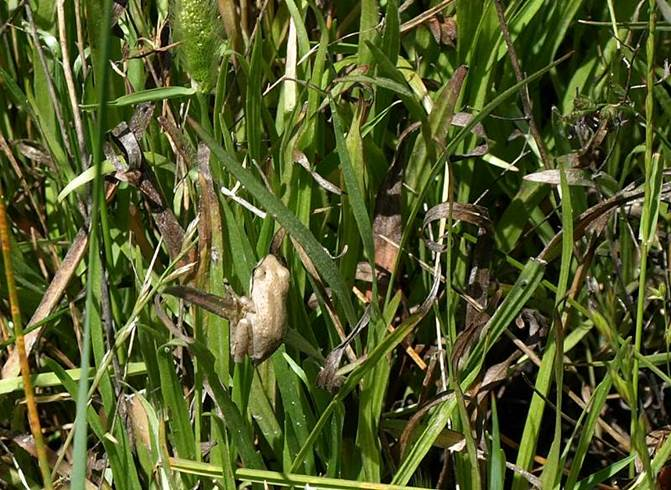
\includegraphics[width=1\textwidth,height=0.75\textwidth]{image/Ch1/unseen_frog_1.jpg}
    \end{subfigure}%
	~~
	      \begin{subfigure}[b]{0.5\textwidth}
           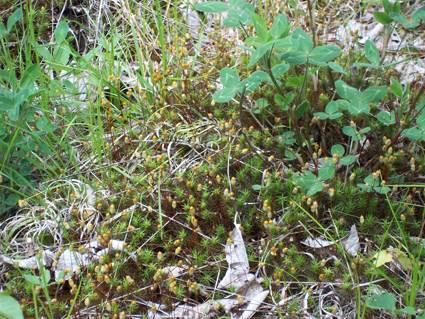
\includegraphics[width=1\textwidth,height=0.75\textwidth]{image/Ch1/unseen_frog_2.jpg}
    \end{subfigure}%
\caption[Photos of frogs]{Photos of frogs to indicate that frogs are difficult to be seen in the field}
\label{fig:Ch1_frogs}       % Give a unique label
\end{figure}



%===============
\section{Basic concepts} 

\subsection{Environment audio data}
The audio data used in this study is mainly derived from two sources: David Stewart's CD \citep{CD} and recordings collected by James Cook University (JCU) \footnote{All the recordings can be obtained from our group website: https://www.ecosounds.org/}. David Stewart's CD is used for the preliminary testing, which is used for the experiment in Chapters \ref{cha:cha4EnhancedFeature} and \ref{cha:cha5Wavelet}. Recordings collected by JCU are used for Chapters \ref{cha:cha6MIML} and \ref{cha:cha7ML}. Firstly, since almost all prior work studied frog recordings with an assumption that only one frog species exists in each individual frog recording, the experiments in Chapter \ref{cha:cha4EnhancedFeature} and \ref{cha:cha5Wavelet} aim to develop a state-of-the-art frog call classification system under this assumption. Secondly, Chapters \ref{cha:cha6MIML} and \ref{cha:cha7ML} focus on the  
study of recordings including multiple overlapping frog vocalisations, which is the real situation for most environment audio data. 


Compared with audio data collected in the laboratories and quiet places (such as David Stewart’s CD), environmental audio data are normally collected under unconstrained noisy conditions (such as JCU recordings). Consequently, the noise and variability issues need to be considered when dealing with environmental audio data. For the background noise, there are a wide variety of non-biological noises and a variety of animal sounds in the environmental recordings. These non-biological noises often come from different sources: rain, wind, human activities (e.g. traffic noise). Besides non-biological noises, many competitive animal sounds (e.g. birds when we are interested in frogs) are also recorded in the environmental audio recordings. In the case of variability, it is produced in many aspects: call structure between species, population of one specific species, time and season changes. All those noises and variabilities make it a challenge to develop a robust frog call classification system.




\subsection{Audio data analysis}
Audio data is usually considered as a mono-dimensional signal. To ease the tasks of understanding, comparison, modification, and resynthesise of signals \citep{rocchesso2003introduction}, audio data analysis is often developed to find the major features representing the time-varying audio data. Many application areas of audio data analysis have been identified: speech processing, mechanical signal processing, bioacoustics analysis, etc. Two most important audio data analysis techniques are Short-time Fourier Transform (STFT) and Linear Predictive Coding (LPC). STFT is a Fourier-related transform, which determines the sinusoidal frequency and phase content of local sections of a signal as it changes over the time \citep{allen1997short}. LPC is mostly used to represent the spectral envelope of an audio data based on the information of a linear predictive model \citep{deng2003speech}. An example of a spectrogram of frog calls derived from a field recording is shown in Figure.~\ref{fig:Ch1_spectrogram}.

\begin{figure}[htb!]
\centering
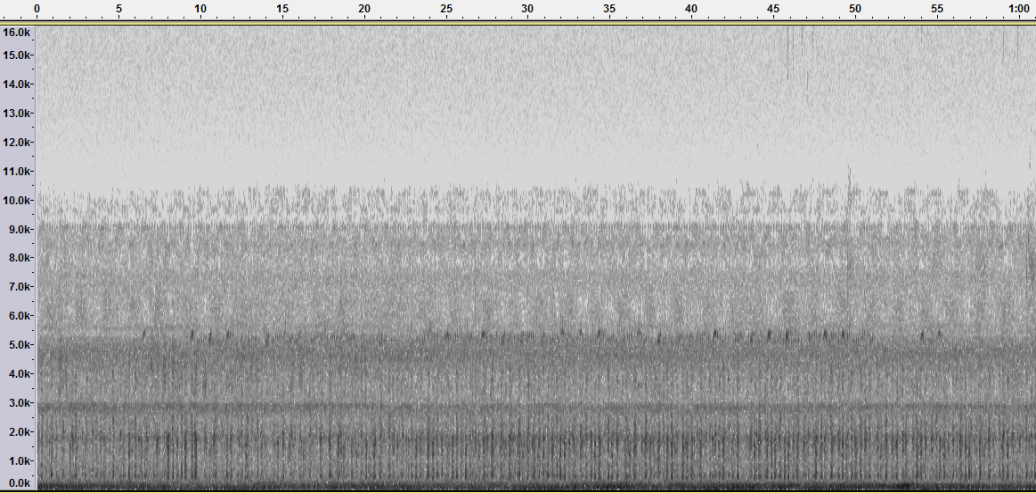
\includegraphics[width=\textwidth]{image/Ch1/spectrogram_example.png}
\caption[An example of spectrogram of environmental recording]{An example of spectrogram of environmental recording. The x-axis is time (seconds); the y-axis is frequency (kHz). The spectrogram is generated from a one-minute recording collected in Townsville, Queensland on around 11.50 pm February 03 2013; the frog species in this recording is \textit{Litoria caerulea}}
\label{fig:Ch1_spectrogram}
\end{figure}





%===================
\subsection{Frog call structure}
Spectrogram (also called sonogram) is a widely used tool for most bioacoustics analysis for its flexible implementation and good applicability. Compared with the hierarchical structure of bird calls, frog calls have a relatively simple call structure \citep{somervuo2006parametric}. The frog vocalisation structure mainly has two ingredients: call and syllable. A frog call is normally made up of several frog syllables (Figure.~\ref{fig:Ch1_spec_mark}).

\begin{figure}[htb!]
\centering
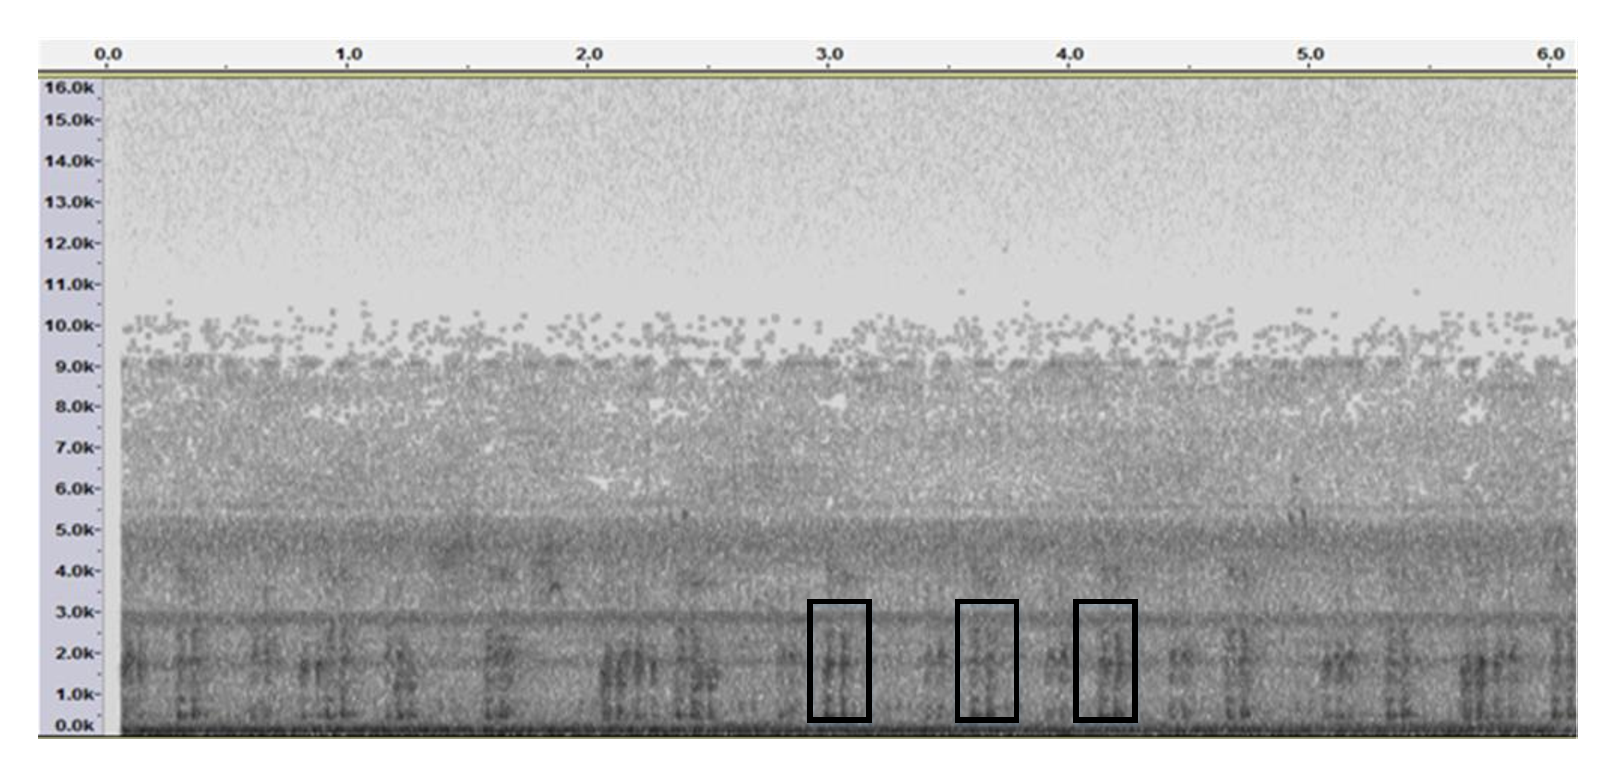
\includegraphics[width=\textwidth]{image/Ch1/spectrogram_mark.pdf}
\caption[Spectrogram of \textit{Litoria caerulea}]{Spectrogram of \textit{Litoria caerulea}, three syllable of \textit{Litoria caerulea} are annotated with one black rectangle, respectively.}
\label{fig:Ch1_spec_mark}
\end{figure}




One syllable is basically a sound that a frog produces with a single blow of air from the lungs \citep{huang2009frog}. For frog call classification, an elementary unit is one syllable. To get an intuitive sense of frog call structure, examples of different frog species in both waveform , spectrogram, and signal-to-noise ratio (SNR) are shown in Table~\ref{tab:wav_spec_cd} and Table~\ref{tab:JCU_para}. For the waveform, x-axis and y-axis represent time and amplitude scales, respectively. The x-axis and y-axis of the spectrogram represent the time and frequency scales, respectively. The grey scale represents the acoustic intensity. Six frog species, which are widely distributed in Queensland, Australia, are selected from David Stewart's CD to generate waveform and spectrogram \citep{CD}. For JCU recordings, eight frog species are selected. The SNR is calculated as follows:

\begin{equation}
SNR=10*log_{10}(\frac{\sum_{i=m}^{m+L}S_{i}^2}{\sum_{j=n}^{n+L}N_{j}^2})
\end{equation}
where $L$ is the length of the signal and noise used for calculating SNR, and set at 6000 samples here, $n$ and $m$ are manual selected start location in the waveform for noise and signal, respectively. 



\begin{table}[htb!]
\centering
\caption[Waveform, spectrogram, and SNR of CD]{Waveform, spectrogram, and SNR of selected six frog species from David Stewart's CD}
\label{tab:wav_spec_cd}
\begin{tabular}{llll}
\hline\hline
\backslashbox{Frog \\ species}{}        & Waveform & Spectrogram & SNR (dB)   \\ \hline
Bufo marinus        &   
\begin{minipage}{.3\textwidth} 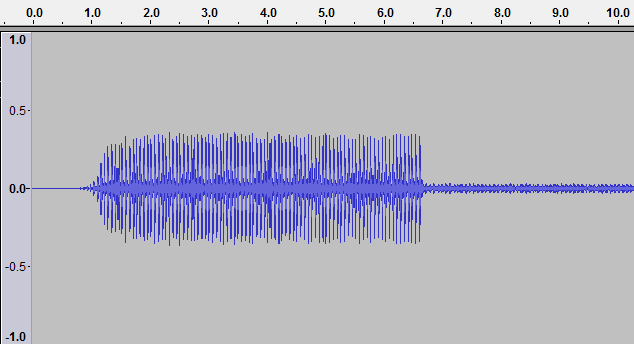
\includegraphics[width=45mm, height=30mm]{image/Ch1/toad_wave.png}  \end{minipage}    &   \begin{minipage}{.3\textwidth} 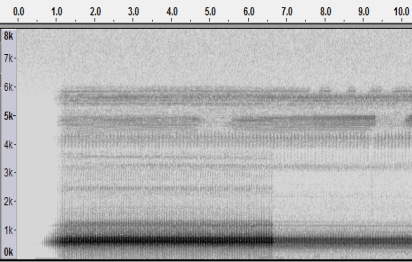
\includegraphics[width=45mm, height=30mm]{image/Ch1/toad_spec.png}  \end{minipage}          & 19.35 \\ \hline
Litoria caerulea    &  \begin{minipage}{.3\textwidth} 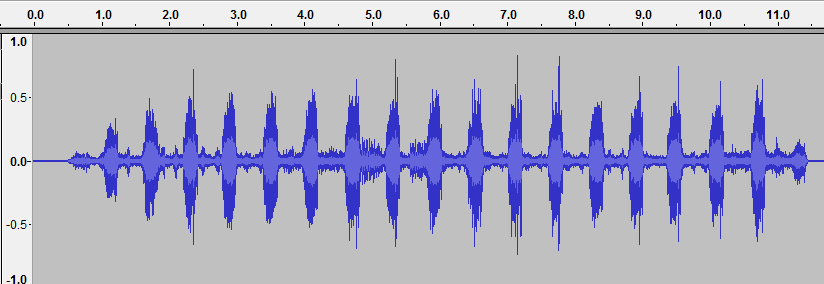
\includegraphics[width=45mm, height=30mm]{image/Ch1/caerulea_wav.png}  \end{minipage}      &     \begin{minipage}{.3\textwidth} 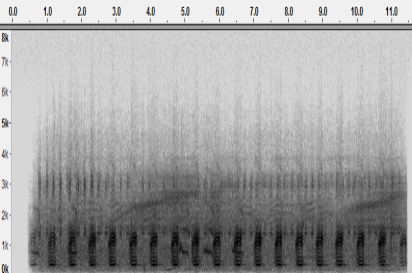
\includegraphics[width=45mm, height=30mm]{image/Ch1/caerulea_spec.png}   \end{minipage}     & 15.78 \\ \hline
Litoria fallax      &      \begin{minipage}{.3\textwidth} 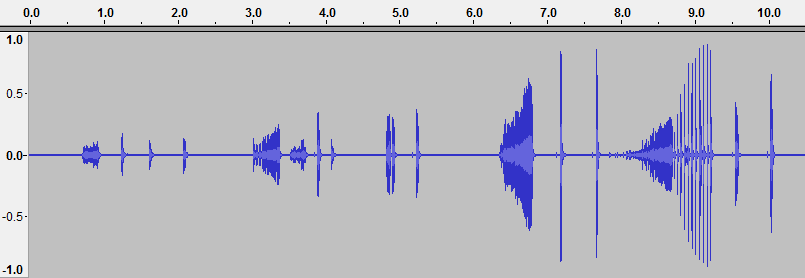
\includegraphics[width=45mm, height=30mm]{image/Ch1/fallax_wav.png} \end{minipage}   &   \begin{minipage}{.3\textwidth} 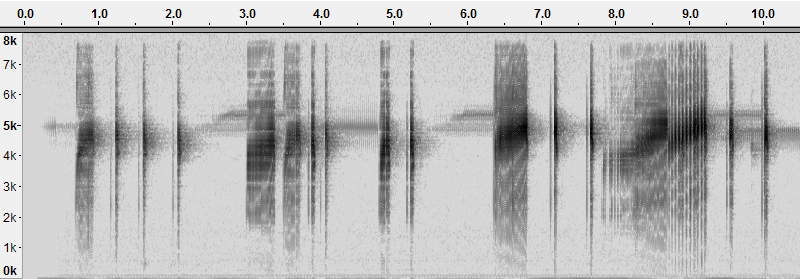
\includegraphics[width=45mm, height=30mm]{image/Ch1/fallax_spec.png}   \end{minipage}       & 43.7  \\ \hline
Litoria gracillenta &     \begin{minipage}{.3\textwidth} 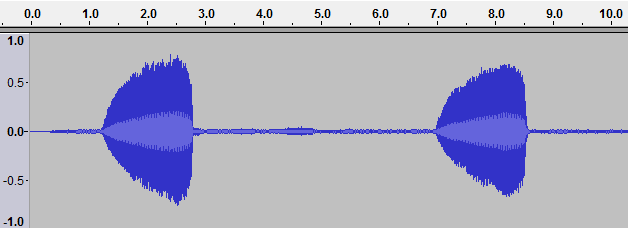
\includegraphics[width=45mm, height=30mm]{image/Ch1/graci_wav.png}  \end{minipage}   &    \begin{minipage}{.3\textwidth} 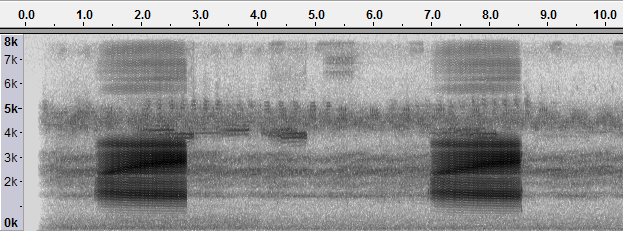
\includegraphics[width=45mm, height=30mm]{image/Ch1/graci_spec.png}     \end{minipage}    & 25.8  \\ \hline
Litoria latopalmata &      \begin{minipage}{.3\textwidth} 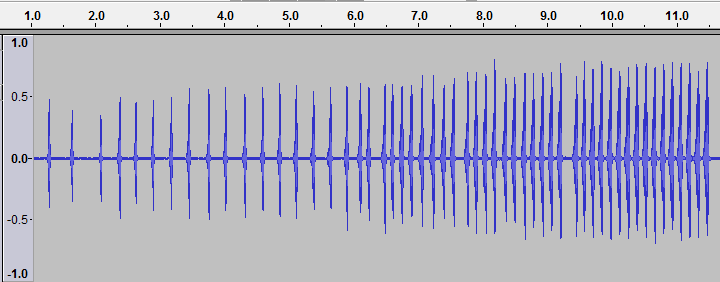
\includegraphics[width=45mm, height=30mm]{image/Ch1/latop_wav.png}  \end{minipage}  &    \begin{minipage}{.3\textwidth} 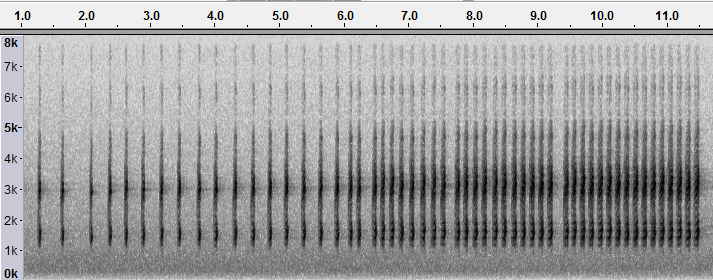
\includegraphics[width=45mm, height=30mm]{image/Ch1/latop_spec.png}    \end{minipage}     & 35.85 \\ \hline
Litoria rubella     &   \begin{minipage}{.3\textwidth} 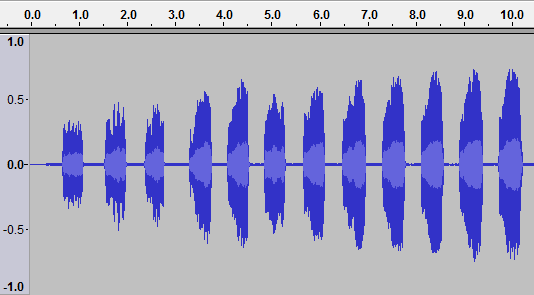
\includegraphics[width=45mm, height=30mm]{image/Ch1/rubella_wav.png}   \end{minipage}    &       \begin{minipage}{.3\textwidth} 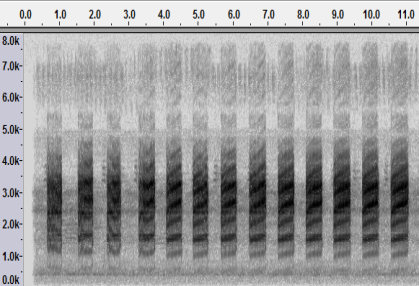
\includegraphics[width=45mm, height=30mm]{image/Ch1/rubella_spec.png}   \end{minipage}   & 36.2  \\ \hline\hline
\end{tabular}
\end{table}



\begin{table}[htb!]
\centering
\caption[Waveform, spectrogram, and SNR of JCU recordings]{Waveform, spectrogram, and SNR of eight frog species (recordings from JCU)}
\label{tab:JCU_para}
\resizebox{\textwidth}{!}{
\begin{tabular}{llll}
\hline\hline
                            & Waveform & Spectrogram & SNR (dB) \\ \hline
Bufo marinus                &   \begin{minipage}{.3\textwidth} 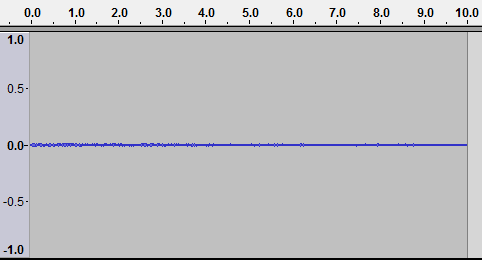
\includegraphics[width=45mm, height=30mm]{image/Ch1/toad_jcu_wav.png}  \end{minipage}       &      \begin{minipage}{.3\textwidth} 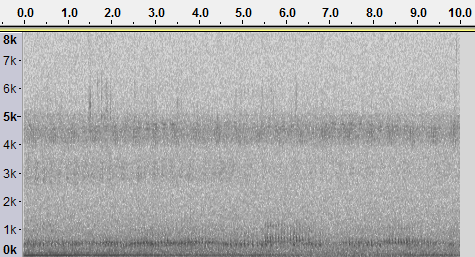
\includegraphics[width=45mm, height=30mm]{image/Ch1/toad_jcu_spec.png}  \end{minipage}       & 1.86     \\ \hline
Cyclorana novaehollandiae   &  \begin{minipage}{.3\textwidth} 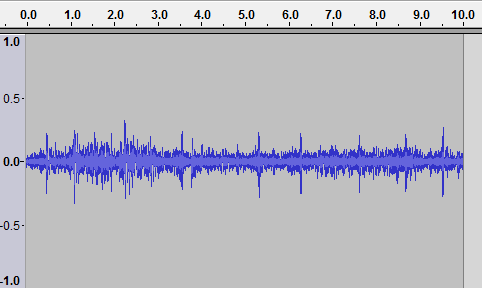
\includegraphics[width=45mm, height=30mm]{image/Ch1/cyc_jcu_wav.png}  \end{minipage}        & \begin{minipage}{.3\textwidth} 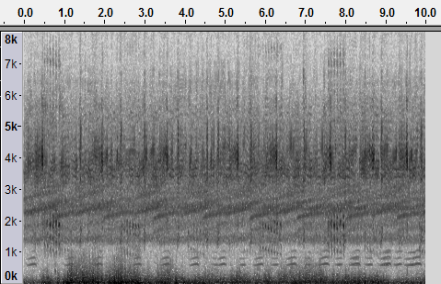
\includegraphics[width=45mm, height=30mm]{image/Ch1/cyc_jcu_spec.png}  \end{minipage}            & -0.13    \\ \hline
Limnodynastes terraereginae &  \begin{minipage}{.3\textwidth} 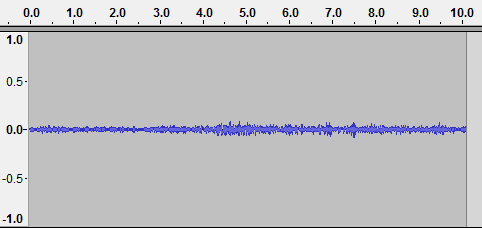
\includegraphics[width=45mm, height=30mm]{image/Ch1/ter_jcu_wav.png}  \end{minipage}        &   \begin{minipage}{.3\textwidth} 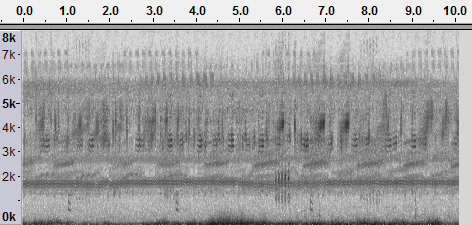
\includegraphics[width=45mm, height=30mm]{image/Ch1/ter_jcu_spec.png}  \end{minipage}          & -2.88    \\ \hline
Litoria fallax              &   \begin{minipage}{.3\textwidth} 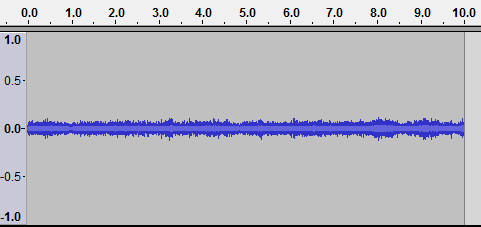
\includegraphics[width=45mm, height=30mm]{image/Ch1/fallax_jcu_wav.png}  \end{minipage}       &    \begin{minipage}{.3\textwidth} 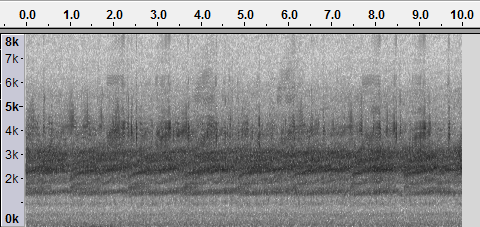
\includegraphics[width=45mm, height=30mm]{image/Ch1/fallax_jcu_spec.png}  \end{minipage}         & 1.52     \\ \hline
Litoria nasuta              &   \begin{minipage}{.3\textwidth} 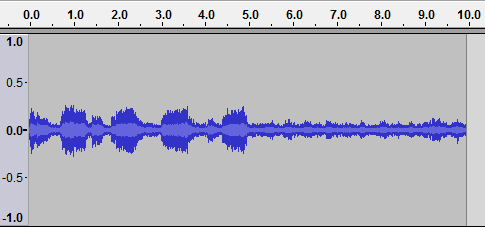
\includegraphics[width=45mm, height=30mm]{image/Ch1/nasuta_jcu_wav.png}  \end{minipage}       &  \begin{minipage}{.3\textwidth} 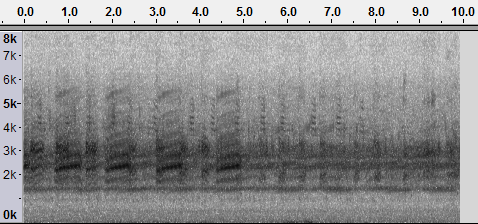
\includegraphics[width=45mm, height=30mm]{image/Ch1/nasuta_jcu_spec.png}  \end{minipage}           & 2.14     \\ \hline
Litoria rothii              &   \begin{minipage}{.3\textwidth} 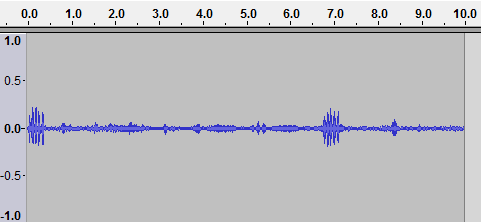
\includegraphics[width=45mm, height=30mm]{image/Ch1/rothii_jcu_wav.png}  \end{minipage}       &    \begin{minipage}{.3\textwidth} 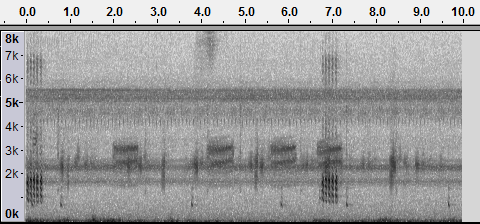
\includegraphics[width=45mm, height=30mm]{image/Ch1/rothii_jcu_spec.png}  \end{minipage}         & 10.24    \\ \hline
Litoria rubella             &    \begin{minipage}{.3\textwidth} 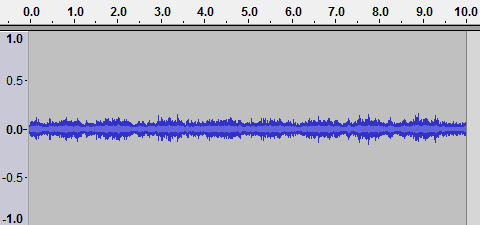
\includegraphics[width=45mm, height=30mm]{image/Ch1/rubella_jcu_wav.png}  \end{minipage}      &   \begin{minipage}{.3\textwidth} 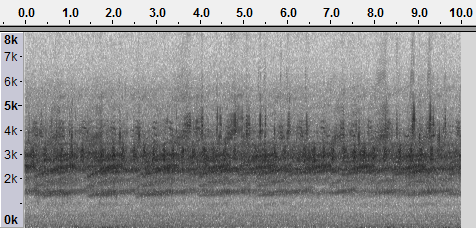
\includegraphics[width=45mm, height=30mm]{image/Ch1/rubella_jcu_spec.png}  \end{minipage}          & 1.08     \\ \hline
Uperolela mimula            &   \begin{minipage}{.3\textwidth} 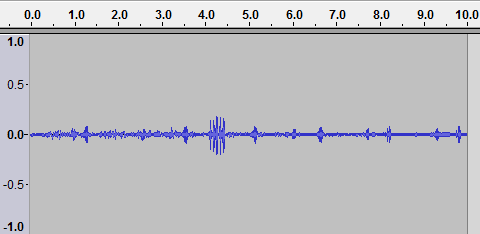
\includegraphics[width=45mm, height=30mm]{image/Ch1/mimula_jcu_wav.png}  \end{minipage}       &  \begin{minipage}{.3\textwidth} 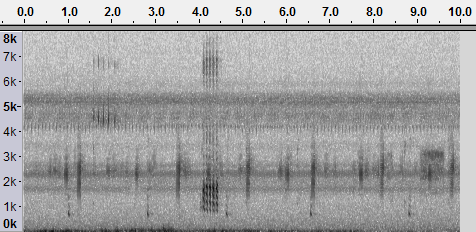
\includegraphics[width=45mm, height=30mm]{image/Ch1/mimula_jcu_spec.png}  \end{minipage}           & 10.28    \\ \hline\hline
\end{tabular}
}
\end{table}


\noindent The parameters of those frog species are shown in Table \ref{tab:cd_parameter}.


\begin{table}[htb!]
\centering
\caption[Averaged parameters of CD]{Averaged parameters of ten syllables of six frog species (David Stewart's CD)}
\label{tab:cd_parameter}
\resizebox{\textwidth}{!}{
\begin{tabular}{llll}\hline\hline
 \backslashbox{Frog \\ species}{Parameters}     & \begin{tabular}[c]{@{}l@{}}Syllable duration \\ (milliseconds)\end{tabular} & Dominant frequency (Hz) & \begin{tabular}[c]{@{}l@{}} Oscillation rate \\ (cycle/second) \end{tabular} \\\hline
Bufo marinus        &    NA   &   600 $\pm$ 30      &                                15 $\pm$ 5 \\
Litoria caerulea    &     500 $\pm$ 30                             &                        500 $\pm$ 75 &    50 $\pm$ 10                             \\
Litoria fallax      &        430 $\pm$ 25                          &                        4700 $\pm$ 450 &                70 $\pm$ 10                 \\
Litoria gracillenta &     430 $\pm$ 25                             &                        4700 $\pm$ 450 &                  70 $\pm$ 10               \\
Litoria latopalmata &       30 $\pm$ 5                           &                        1400 $\pm$ 120 &       5 $\pm$ 2                          \\
Litoria rubella     &   160 $\pm$ 15                               &                        4100 $\pm$ 380 &                            70 $\pm$ 10    \\\hline\hline
\end{tabular}
}
\end{table}




Since the signal power and background noise in this study vary from recordings to recordings and calls to calls within the recording, Table~\ref{tab:CI_CD} and Table~\ref{tab:CI_JCU} calculate the confidence intervals of high and low SNR recordings for the power of signal and noise. The calculation of confidence interval is defined as follows:

\begin{equation}
CI=\mu \pm Z*\frac{\sigma}{\sqrt{L}}
\end{equation}
where $\mu$ and $\sigma$ are the mean and standard deviation, respectively, $Z$ is the upper $\frac{(1-C)}{2}$ critical value for the standard normal distribution, $C$ is the confidence level, and set at 0.95.




\begin{table}[htb!]
\centering
\caption[Confidence interval for CD]{Confidence interval of signal and noise (David Stewart's CD)}
\label{tab:CI_CD}
\begin{tabular}{lll}
\hline\hline
    \backslashbox{Frog \\ species}{Parameters}                      & Confidence intervals of signal & Confidence intervals of noise \\ \hline
Bufo marinus        &  -9.27*$10^{-6}$ $\pm$ 2.10*$10^{-3}$ &  -2.67*$10^{-5}$ $\pm$ 2.26*$10^{-4}$                             \\ 
Litoria caerulea    &      -6.73*$10^{-5}$ $\pm$ 2.40*$10^{-3}$     &                              -6.89*$10^{-5}$ $\pm$ 3.90*$10^{-4}$ \\ 
Litoria fallax      &   -5.85*$10^{-6}$ $\pm$ 1.50*$10^{-3}$                             &                              -2.73*$10^{-5}$ $\pm$ 9.62*$10^{-6}$ \\ 
Litoria gracillenta &     -7.12*$10^{-5}$ $\pm$ 2.00*$10^{-3}$                           &                              -7.70* $10^{-5}$ $\pm$ 1.00*$10^{-4}$ \\ 
Litoria latopalmata &   -6.58*$10^{-5}$ $\pm$ 2.70*$10^{-3}$                            &                              -1.02*$10^{-4}$ $\pm$ 4.36*$10^{-5}$ \\ 
Litoria rubella     &   -3.13*$10^{-5}$ $\pm$ 3.00*$10^{-3}$                           &                              -9.87*$10^{-5}$ $\pm$ 4.70*$10^{-5}$ \\ \hline\hline
\end{tabular}
\end{table}




\begin{table}[htb!]
\centering
\caption[Confidence interval for JCU recordings]{Confidence interval of signal and noise for JCU recordings}
\label{tab:CI_JCU}
\begin{tabular}{lll}
\hline\hline
   \backslashbox{Frog \\ species}{Parameters}                          & Confidence intervals of signal & Confidence intervals of noise \\ \hline
Bufo marinus                &   -1.36*$10^{-5}$ $\pm$ 6.00*$10^{-5}$                             &                              -3.22*$10^{-5}$ $\pm$ 4.80*$10^{-5}$ \\ \hline
Cyclorana novaehollandiae   &    1.30*$10^{-3}$ $\pm$ 8.70*$10^{-4}$                            &                              1.30*$10^{-3}$ $\pm$ 8.90*$10^{-4}$ \\ \hline
Limnodynastes terraereginae &       6.43*$10^{-5}$ $\pm$  1.30*$10^{-4}$                         &                              1.86*$10^{-4}$ $\pm$ 1.89*$10^{-4}$ \\ \hline
Litoria fallax              &  2.31*$10^{-5}$ $\pm$ 5.00*$10^{-4}$                              &                              5.75*$10^{-6}$ $\pm$ 4.22*$10^{-4}$ \\ \hline
Litoria nasuta              &                  -1.55*$10^{-4}$ $\pm$ 4.90* $10^{-4}$              &                              6.25* $10^{-6}$ $\pm$ 3.85*$10^{-4}$ \\ \hline
Litoria rothii              &              -3.32*$10^{-4}$ $\pm$ 9.2*$10^{-4}$                  &                              1.61* $10^{-4}$ $\pm$ 2.84*$10^{-4}$ \\ \hline
Litoria rubella             &      -8.15*$10^{-5}$ $\pm$ 5.52*$10^{-4}$                          &                              -2.69* $10^{-5}$ $\pm$ 4.87*$10^{-4}$ \\ \hline
Uperolela mimula            &             -1.20*$10^{-3}$  $\pm$ 1.10*$10^{-3}$                   &                              -9.36*$10^{-4}$ $\pm$ 3.35*$10^{-4}$ \\ \hline\hline
\end{tabular}
\end{table}




\subsection{Acoustic event and background noise}


An acoustic event is a localised region of high intensity in a spectrogram. As we can see from Figure.~\ref{fig:label}, there are lots of acoustic events in one-minute recording. This study focuses on the frog vocalisations, and frog calls are recorded as signals. Consequently, all the other events are called background noise, whose definition is ambiguous. In this study, both high and low SNR recordings are investigated to build a robust frog call classification system. Most previous studies present the frog call classification system using the high SNR recordings. The high SNR recordings often assume that there is only one frog species in each individual recording with few background noises ($SNR \geq 15 dB$). In contrast, most low SNR recordings consist of more than one frog species in an individual recording with lots of background noises ($SNR \leq 15 dB$). For the low SNR recordings, Table~\ref{tab:psd} show the power spectral density of signal and noise. It can be seen that the noises in low SNR recordings are often generated by several sources and broadband, which cover different frequency bands and lead to the frequency overlapping between the signal and noise. Therefore, it is challenging to analyse the recordings containing background noise and simultaneous vocalising events.




\begin{table}[htb!]
\centering
\caption[PSD of JCU recordings]{Power spectral density (PSD) estimate of signal and noise (JCU recordings); for some frog species, the PSD difference between the signal and background noise is marked with the red rectangle, which indicates the frequency location of specific frog species; for others, the PSD of signal and noise is very similar, which means that some sources have similar frequency information with frog species}
\label{tab:psd}
\resizebox{\textwidth}{!}{
\begin{tabular}{lll}
\hline\hline
  \backslashbox{Frog \\ species}{Parameters}                           & Welch PSD (Signal) & Welch PSD estimate (Noise) \\ \hline
Bufo marinus                &  \begin{minipage}{.3\textwidth} 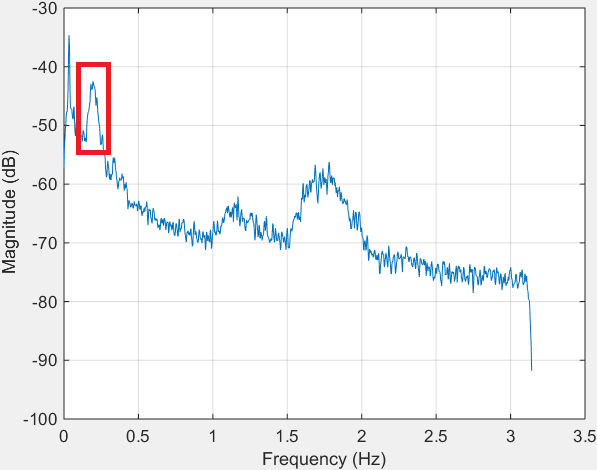
\includegraphics[width=45mm, height=35mm]{image/Ch1/1_signal.png}  \end{minipage}       &      \begin{minipage}{.3\textwidth} 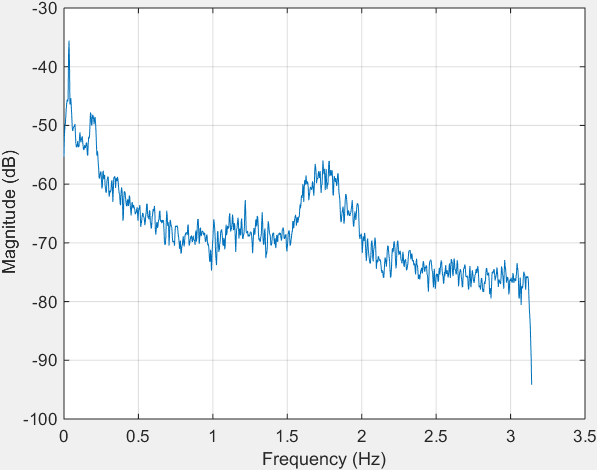
\includegraphics[width=45mm, height=35mm]{image/Ch1/1_noise.png}  \end{minipage}          \\ \hline
\begin{tabular}[c]{@{}l@{}} Cyclorana \\ novaehollandiae  \end{tabular}    & \begin{minipage}{.3\textwidth} 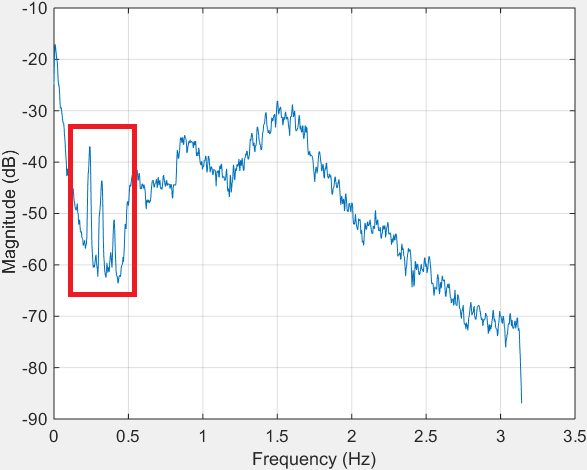
\includegraphics[width=45mm, height=35mm]{image/Ch1/2_signal.png}  \end{minipage}                              &                                              \begin{minipage}{.3\textwidth} 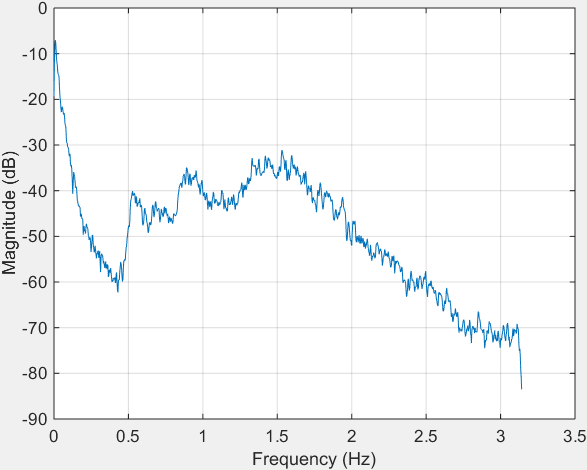
\includegraphics[width=45mm, height=35mm]{image/Ch1/2_noise.png}  \end{minipage}   \\ \hline
 \begin{tabular}[c]{@{}l@{}} Limnodynastes \\ terraereginae  \end{tabular}  &  \begin{minipage}{.3\textwidth} 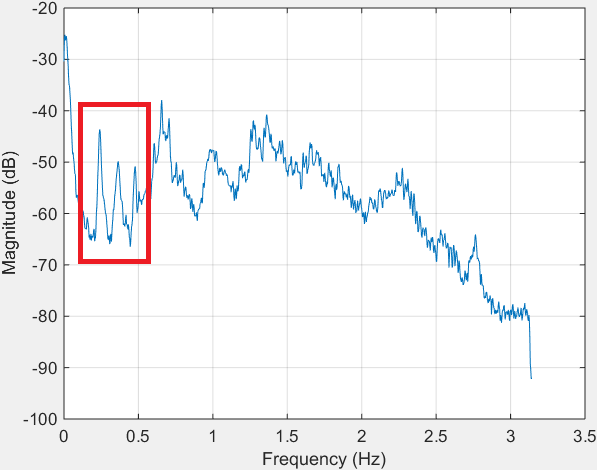
\includegraphics[width=45mm, height=35mm]{image/Ch1/3_signal.png}  \end{minipage}                              &                                             \begin{minipage}{.3\textwidth} 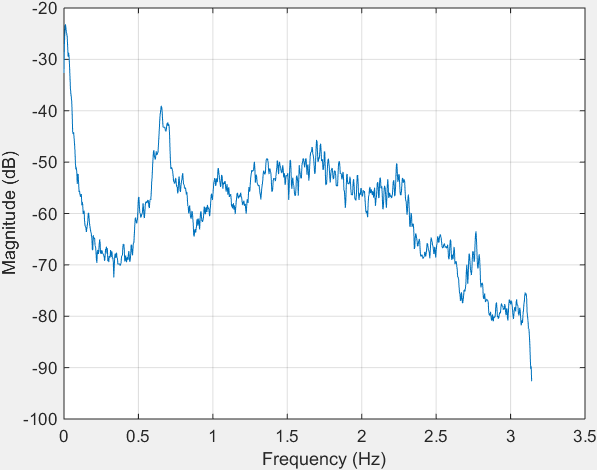
\includegraphics[width=45mm, height=35mm]{image/Ch1/3_noise.png}  \end{minipage}   \\ \hline
Litoria fallax              & \begin{minipage}{.3\textwidth} 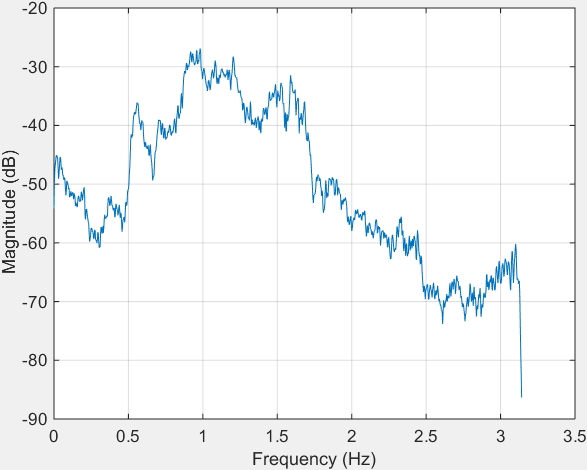
\includegraphics[width=45mm, height=35mm]{image/Ch1/4_signal.png}  \end{minipage}                             &                                               \begin{minipage}{.3\textwidth} 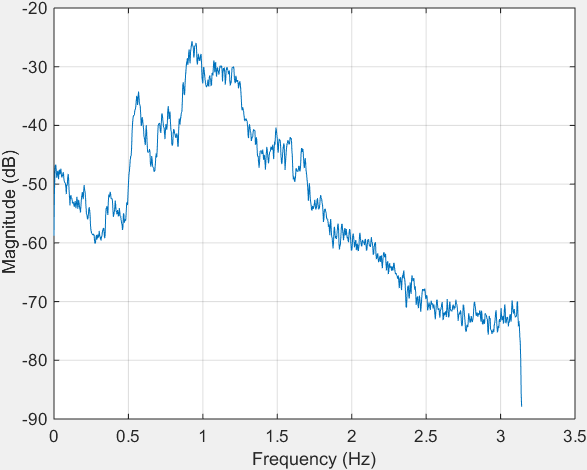
\includegraphics[width=45mm, height=35mm]{image/Ch1/4_noise.png}  \end{minipage} \\ \hline
Litoria nasuta              &   \begin{minipage}{.3\textwidth} 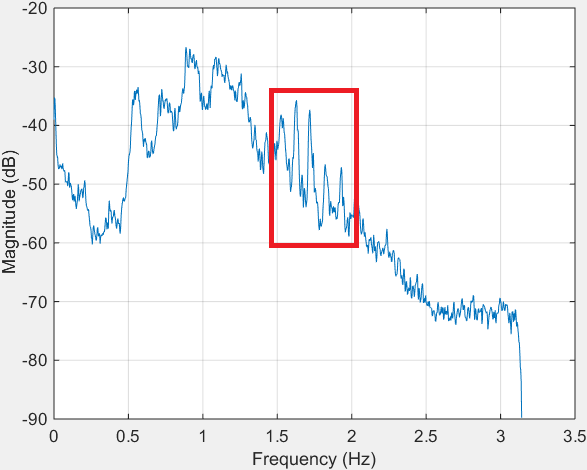
\includegraphics[width=45mm, height=35mm]{image/Ch1/5_signal.png}  \end{minipage}                           &                                               \begin{minipage}{.3\textwidth} 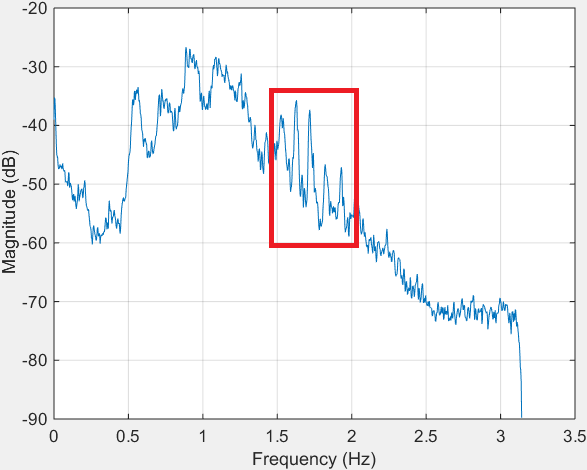
\includegraphics[width=45mm, height=35mm]{image/Ch1/5_signal.png}  \end{minipage} \\ \hline
\end{tabular}
}
\end{table}


\begin{table}[htb!]
\centering
\resizebox{\textwidth}{!}{
\begin{tabular}{lll}
\hline
Litoria rothii              &  \begin{minipage}{.3\textwidth} 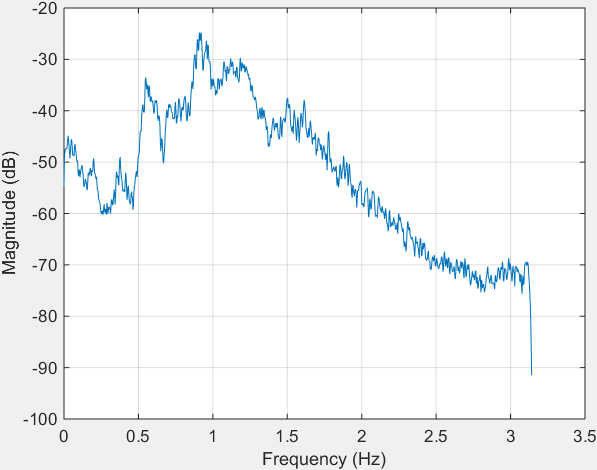
\includegraphics[width=45mm, height=35mm]{image/Ch1/6_signal.png}  \end{minipage}                         &    \begin{minipage}{.3\textwidth} 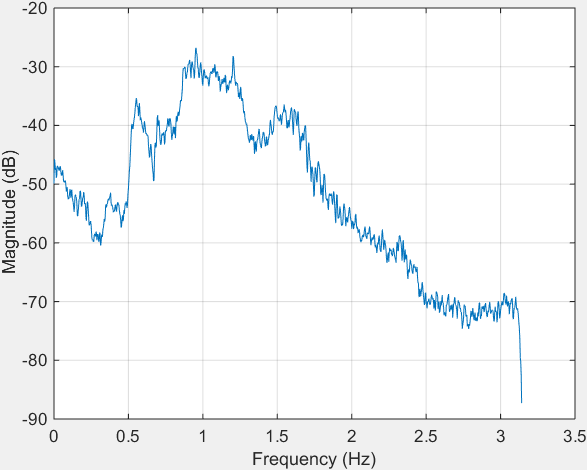
\includegraphics[width=45mm, height=35mm]{image/Ch1/6_noise.png}  \end{minipage}                                           \\ \hline
Litoria rubella             &    \begin{minipage}{.3\textwidth} 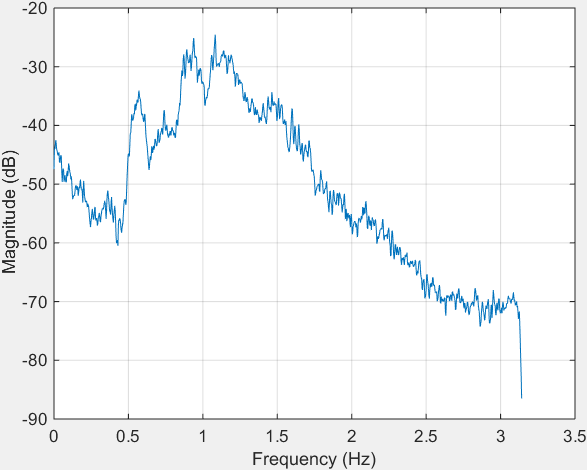
\includegraphics[width=45mm, height=35mm]{image/Ch1/7_signal.png}  \end{minipage}                               &                                               \begin{minipage}{.3\textwidth} 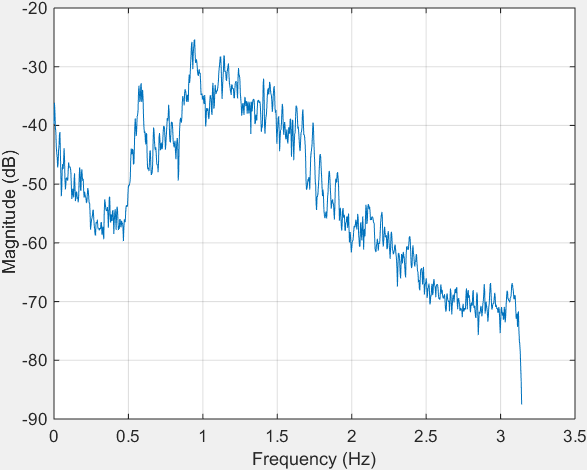
\includegraphics[width=45mm, height=35mm]{image/Ch1/7_noise.png}  \end{minipage} \\ \hline
Uperolela mimula            &   \begin{minipage}{.3\textwidth} 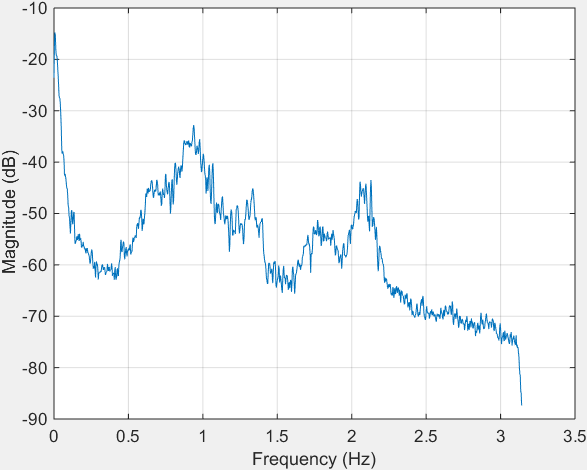
\includegraphics[width=45mm, height=35mm]{image/Ch1/8_signal.png}  \end{minipage}                              &                                             \begin{minipage}{.3\textwidth} 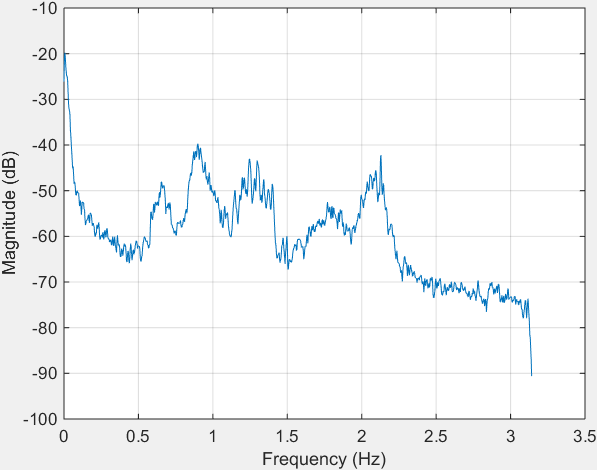
\includegraphics[width=45mm, height=35mm]{image/Ch1/8_noise.png}  \end{minipage} \\ \hline\hline
\end{tabular}
}
\end{table}

\subsection{Frog call classification}

For a frog call classification system, it often consists of four parts (Figure.~\ref{fig:Ch1_flowchart}) : (1) pre-processing, which includes signal processing and noise reduction; (2) syllable segmentation, which is used to generate basic classification unit for frog calls; (3) feature extraction; (4) classification.  



\begin{figure}[htb!]
\centering
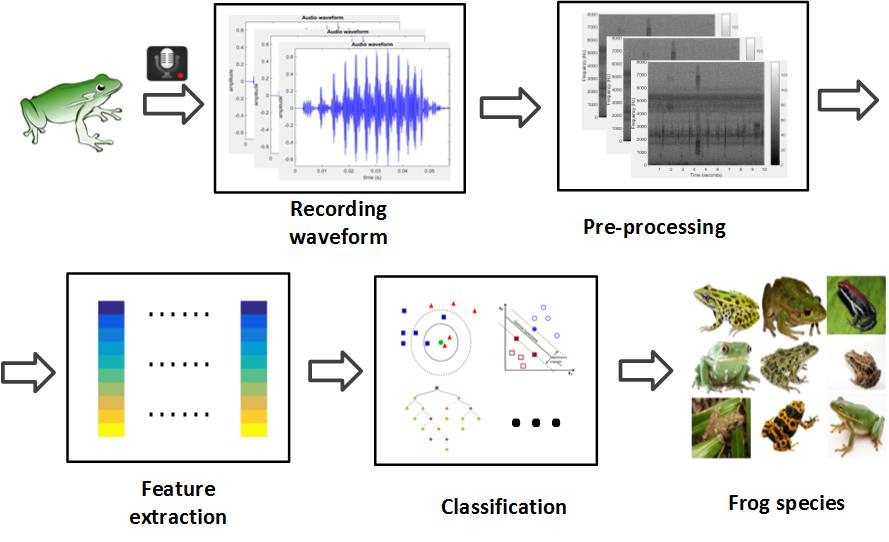
\includegraphics[width=\textwidth]{image/Ch1/flowchart.jpg}
\caption[Flowchart of frog call classification]{Flowchart of frog call classification}
\label{fig:Ch1_flowchart}
\end{figure}


\subsection{Research problem}
Most datasets used in previous frog call classification studies assumes that there is only one frog species exist in each individual recordings. However, these resulting frog calls cannot reflect the characteristics of frog vocalisations in real-world situations, such as background noise, frog chorus. To develop a robust frog call classification system for environmental recordings, two main challenges have been identified. 


\noindent \textbf{Challenge 1}: Most previous work studied frog call classification using high SNR recordings, the first challenge is thus to further improve the classification performance using high SNR recordings. Various acoustic features have been investigated for the classification of frog calls in high SNR recordings. Since our work finally aims to classify frog calls in low SNR recordings, most features that can successfully classify high SNR recordings cannot perform well for low SNR recordings. Consequently, it is still a big challenge to develop robust acoustic features to classify frog species in low SNR recordings. 

\noindent \textbf{Challenge 2}: Another challenge is the classification framework for studying frog vocalisations in low SNR recordings. Since most previous work assumed that each individual recording consists of only one frog species, a single-instance single-label (SISL) framework is suitable for classifying frog calls in those recordings. However, due to the different characters of low SNR recordings, which consist of more than one frog species, the SISL framework is no longer suitable. Therefore, different classification frameworks need to be investigated to study frog vocalisations in low SNR recordings.



\subsection{Research questions}
The research questions are developed in order to solve the aforementioned problems, which can be categorised into three parts. 

 \begin{enumerate}
     \item which acoustic features used for addressing high SNR recordings can be transplanted to study low SNR recordings?
     \item How to develop acoustic features to classify frog calls in low SNR recordings?
     \item How to adopt machine learning techniques to classify simultaneous overlapping frog calls?
  \end{enumerate}




\subsection{Aims and objectives}
This thesis aims to develop a robust frog call classification system to monitor the environment. For high SNR recordings, we want to improve the classification performance. As for the low SNR recordings, we plan to design novel frameworks to classify multiple simultaneously vocalising frog species. With our classification results, ecologists can then make decisions on how to protect and improve the health of frog populations. The specific research objectives are listed below.


\begin{enumerate}

\item	To improve the current representation schemes for modelling frog calls in high SNR recordings

\item 	To develop robust feature extraction methods for low SNR recordings for frog call classification

\item   To investigate machine learning techniques (MIML learning and ML learning) to tackle the frog call classification problem in low SNR recordings

\end{enumerate}
 
 
 
\subsection{Significance and contributions}
For the development of sensor techniques, acoustic sensors have been widely deployed in the field for surveying vocalising animals. Different from recordings collected in the constrained environment, recordings collected in the field often have low SNR and consist of multiple simultaneous vocalising frog species. In this dissertation, we first investigate the high SNR recordings to further improve the classification performance of frog recordings with high SNR. 
Then, those features that can be used for studying frog calls in low SNR recordings are transplanted from high SNR recordings for further analysis.
Since field recordings often consists of multiple simultaneous vocalising frog species, both MIML and ML learning are used for the classification of those low SNR field recordings. Meanwhile, the frog calling activity can also be monitored based on the MIML and ML classification results.
With our developed frog call classification frameworks, ecologists can then analyse frogs by collecting audio data. It will significantly reduce the expert labour cost for monitoring frog calling activity of a particular area. The monitoring result can also help reveal the importance of environment protection, which can be achieved via studying the correlation between the frog calling activity and weather variables. 

 
 
\subsection{Thesis structure} 
 
This thesis consists of eight chapters. Chapter \ref{cha:cha1Introduction} described the background, motivation and contributions of the thesis. Chapter \ref{cha:cha2LiteratureReview} reviews the literature related to frog call classification. Chapter \ref{cha:cha3Method} discusses a number of feature extraction approaches in detail. Also various classification techniques used in this research will be explained, so one can understand the strategy employed for each classifier. Chapter \ref{cha:cha4EnhancedFeature} discusses the implementation of frog call classification by syllable features. Chapter \ref{cha:cha5Wavelet} discusses wavelet analysis for frog call classification. Chapter \ref{cha:cha6MIML} discusses the use of multiple-instance multiple-label framework for frog call classification. Chapter \ref{cha:cha7ML} discusses the multiple-label learning for frog call classification. Chapter \ref{cha:cha8Conclusions} concludes this research and recommends possible directions in future work.

        %Ch1Introduction.tex
% Ch2LiteratureReview.tex

\chapter[Literature Review]{Literature Review}
\label{cha:cha2LiteratureReview}

This chapter reviews the extant literature on frog call classification. 
It aims to give a quantitative and detailed analysis of related techniques used in frog call classification.    

\section{Introduction}
\label{intro}
Over the past decade, frog biodiversity has rapidly declined because of frogs' sensitive to habitat loss and degradation, introduced invasive species, and environmental pollution \citep{dudgeon2006freshwater}. On one hand, frog biodiversity is rapidly declining, and on the other frogs are greatly valuable for the environment. Firstly, frogs are an integral part of the food web, and the decline of their population can result in negative impacts through the whole ecosystem. Secondly, frogs are famous indicator species for environment health. Finally, frogs are very useful in medical research that benefit human \footnote{http://www.savethefrogs.com/why-frogs}. The rapid biodiversity decline and great importance of frogs make it necessary for frog biodiversity monitoring to increase. 

To monitor the change of frog biodiversity and optimise the protection policy, many researchers have shown interest in studying frogs. Compared to counting frogs by visual observation, hearing the vocalisations of frogs is much easier. Consequently, frog vocalisations are often used for monitoring frogs. There are two approaches for acoustic frog monitoring. The traditional field survey methods require ecologists to physically visit sites to collect acoustic data, which are both time-consuming and costly. In contrast, recent advances in acoustic sensor techniques have greatly extended the spatio-temporal scale for acoustic monitoring of frog biodiversity \citep{wimmer2013analysing}. The large volumes of acoustic data collected this way make it essential to develop new automated methods of analysis. 


Over the last few years, many researchers have described automated methods for detecting and classifying frog calls \citep{huang2008realization, huang2009frog, han2011acoustic,chen2012automatic, Gingras2013, camacho2013automatic, Huang20141, Xie1504:Acoustic}. However, there is no paper that summarises those methods. In this work, we present a comprehensive survey of frog call classification to provide acoustic signal researchers with basic information, current methods and trends in this field. 

Three parts play important roles in the performance and precision of frog call classification: signal pre-processing, feature extraction, and classification. In this survey, these three important parts of frog call classification are presented as shown in Fig.~\ref{fig:flowchart}. 


Signal pre-processing consists of signal processing, noise reduction and syllable segmentation. Signal processing often denotes changing a signal from one-dimension (audio data) into two-dimensional representation (image). Noise reduction is essential to improve the classification performance. Since the elementary acoustic unit for frog call classification is the syllable, which is a continuous vocalization emitted by an individual, segmenting continuous recordings of frog calls into individual syllables is necessary. 

Previous studies have developed various methods for feature extraction \citep{huang2008realization, huang2009frog, han2011acoustic, chen2012automatic, Gingras2013, camacho2013automatic, Huang20141, Xie1504:Acoustic}. Here we review and analyse all the used features: time domain and frequency domain features, 
time-frequency features, cepstral features, and other features. After feature extraction, numerous classifiers have been proposed for frog call classification. A summary of those classifiers is given in section \ref{classifiers}.


It is worth noting that most previous researchers used different databases for their experiments because frog call research is often related to geographical regions \citep{jang2011geographic}. Consequently, there is still a lack of uniformity in the way classification methods are evaluated and assessed. This survey is not meant to compare all previous frog call classification methods and find the best one, but to assemble all the methods to provide other researchers with a direction for the classification of frog calls. To be specific, we mainly survey different features used for frog call classification because most studies focus on new features rather than new signal processing techniques, syllable segmentation methods, or classifiers.

%\begin{figure*}[htb!]
%\centering
%    \begin{subfigure}[b]{\textwidth}
%           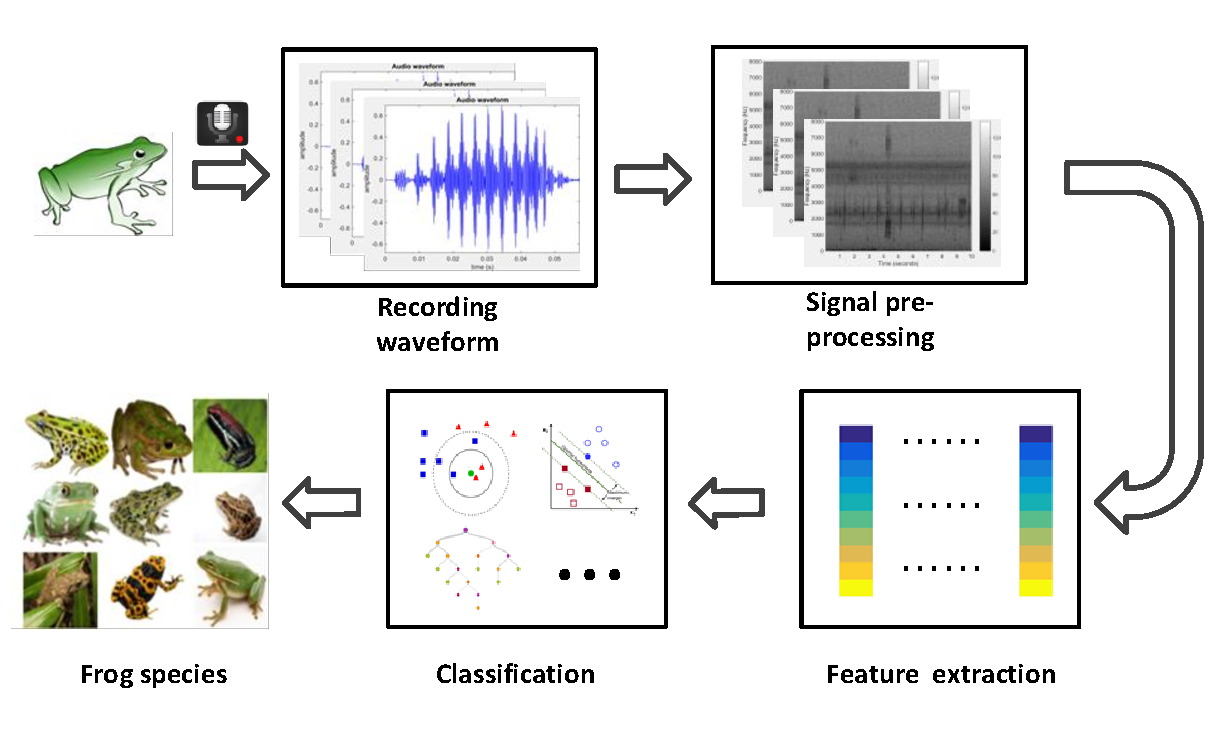
\includegraphics[width=\textwidth]{image/flowchart.pdf}
%    \end{subfigure}%
%\caption{Flowchart of frog call classification: pre-processing, feature extraction, and classification.}
%\label{fig:flowchart}       
%\end{figure*}


The remainder of this survey is organised as follows: In section \ref{pre-processing}, signal pre-processing is presented in its three parts: signal processing, noise reduction, and syllable segmentation. 
In section \ref{features}, different acoustic features are investigated for frog call classification. In section \ref{classifiers}, numerous classifiers are studied for frog call classification. In section \ref{experiment}, experimental results of state-of-the-art research are discussed. Finally, the discussion and conclusion are given in sections \ref{discussion} and \ref{conclusion}, respectively.




\section{Signal pre-processing}
\label{pre-processing}

For frog call classification, signal pre-processing is the first step after acoustic data is collected. It often consists of signal processing, noise reduction, and syllable segmentation. Each part of signal pre-processing is described below.


\subsection{Signal processing}
Signal processing often denotes the transformation of frog calls from one-dimension (recording waveform) to two dimensions (time-frequency representation). Many techniques have been developed for this transformation including short-time Fourier transform (STFT) \citep{STFT1977}, Wigner-Ville distribution \citep{WV1987}, and wavelet transform \citep{meyer1995wavelets}. STFT is the most widely used technique among them for its flexible implementation and better applicability. Given one frog call $x(t)$, its fast Fourier transform can be expressed as
\begin{equation}
X(k) = \sum_{n=0}^{L-1}x(n)w(n)e^{-j2 \pi kn/L}, 0 \leq k \leq L-1
\end{equation}
where $X(k)$ is the frequency domain signal (spectrum) and denotes each frame of the spectrogram, and $w(n)$ is the window function. The waveform, spectrum and spectrogram of one individual syllable for \textit{Mixophyes fasciolatus} is illustrated in Fig.~\ref{fig:spectrogram}. Here three representations are consistent with features in three domains: the time domain, frequency domain and time-frequency domain.

\begin{figure*}[htb!]
\centering
      \begin{subfigure}[b]{0.32\textwidth}
           \includegraphics[width=1\textwidth,height=0.75\textwidth]{image/LR/waveform.pdf}
    \end{subfigure}%
	~
	      \begin{subfigure}[b]{0.32\textwidth}
           \includegraphics[width=1\textwidth,height=0.75\textwidth]{image/LR/spectrum.pdf}
    \end{subfigure}%
	~
    \begin{subfigure}[b]{0.32\textwidth}
           \includegraphics[width=1\textwidth,height=0.75\textwidth]{image/LR/spectrogram.pdf}
    \end{subfigure}%
\caption[Waveform, spectrum and spectrogram of one frog syllable]{Waveform, spectrum and spectrogram of one frog syllable for \textit{Mixophyes fasciolatus}. The window function, size and overlap are Hamming window, 128 samples and 85\%, respectively}
\label{fig:spectrogram}       % Give a unique label
\end{figure*}


%So far, wavelet packet decomposition (WPD) is the another technique that applied for frog call classification \citep{jie2015escience}. However, different from 

%Besides STFT, Xie et al recently introduced . 
%Compared with STFT, WPD has a better frequency resolution.


\subsection{Noise reduction}
Noise reduction is an optional process for frog call classification. 
\cite{Huang20141} applied a de-noise filter for noise reduction. The wavelet threshold function in the one-dimensional signal was used as the filter kernel function.
\cite{bedoya2014automatic} introduced spectral noise gating method for noise reduction. Specifically, the selected frequency band spectrum of the frogs' call to be detected was estimated and suppressed. \cite{emr2015Xie} used Wiener filtering to remove the background graininess, then applied spectral subtraction to the filtered spectrogram using a modified method from the adaptive level equalization algorithm. While the aforementioned noise reduction methods can remove some background noise, some of the desired signals will be suppressed. Noise reduction methods are therefore selectively used based on signal-to-noise ratio of the acoustic data and the research problem.




\subsection{Syllable segmentation}
For frog calls, the basic elementary acoustic unit is a syllable, which is a continuous frog vocalisation emitted by an individual frog \citep{huang2009frog}. The precision of syllable segmentation will directly affect the classification performance, since features used for frog call classification are calculated based on each syllable. Frog syllable segmentation methods in previous studies are summarised and listed in Table \ref{tab:segmentation}. All previous methods except \citep{jie2015ICIP} cannot address recordings with simultaneous vocalising frog calls. Meanwhile, those methods that used the time domain feature for segmentation, cannot address recordings with low signal-to-noise ratio. \cite{jie2015ICIP} introduced an unsupervised learning method, which included multiple image processing techniques for syllable segmentation. However, the downside of this unsupervised process was that not all segmented syllables correspond to frog vocalisations.

%Since the accuracy of segmentation results directly affect the final classification accuracy \citep{Colonna20157367}, meanwhile we focus on the evaluation of different features for frog call classification in this survey, we manually segment the frog calls for reducing the effect of segmentation result for classification accuracy,
  
\begin{table}[htb!]
\centering
\caption[Summary of related work]{Summary of related work for frog syllable segmentation. Here, E denotes energy, ZCR denotes zero-crossing rate.}
\label{tab:segmentation}
\resizebox{\textwidth}{!}{
\begin{tabular}{lll}
\hline\hline
{\bf Authors} & {\bf Features for segmentation}                    & {\bf Procedure}                          \\ \hline
   \citet{han2011acoustic}            & Spectral entropy                  & Manual                                      \\ 
  \citet{jaafar2013}             & E and ZCR                         & Sequential                \\ 
    \citet{huang2009frog}           & Amplitude                         & Non-sequential                           \\ 
    \citet{chen2012automatic}           & Spectrogram                         & Non-sequential            \\ 
     \citet{Xie1504:Acoustic}          & Spectrogram                       & Non-sequential           \\ 
     \citet{Colonna20157367}          & Incremental E and Incremental ZCR & Sequential and real time      \\
     \citet{jie2015ICIP}   &    Image processing    & Non-sequential    \\    
      \hline\hline
\end{tabular}
}
\end{table}




\section{Acoustic features for frog call classification}
\label{features}
Developing effective acoustic features that show greater variation between rather than within species is important for achieving robust classification results \citep{Fox20081187}. For frog call classification, acoustic features can be classified into four categories: time domain and frequency domain features, time-frequency domain features, cepstral features, and other features. 

\subsection{Time domain and frequency domain features for frog call classification}

Time domain features for frog call classification have been explored for a long time \citep{huang2008realization, huang2009frog, dayou2011classification, chen2012automatic, camacho2013automatic, Huang20141}. Time domain features are often combined with frequency domain features for frog call classification.
 
\cite{huang2009frog} used spectral centroid, signal bandwidth, and threshold-crossing rate for frog call classification with a k-nearest neighbour classifier (k-NN) and support vector machines (SVM). In another work, \cite{Huang20141} combined spectral centroid, signal bandwidth, spectral roll-off, threshold-crossing rate, spectral flatness, and average energy to classify frog calls using neural networks. Another paper published by  \citep{huang2008realization} used spectral centroid, signal bandwidth, spectral roll-off, and threshold-crossing rate for frog call classification. 
\cite{dayou2011classification} combined Shannon entropy, R$\acute{e}$nyi entropy and Tsallis entropy for frog call classification. Based on this work,  \cite{han2011acoustic} improved the classification accuracy by replacing Tsallis entropy with spectral centroid.
To classify anurans into four genera, a three-parameter model was proposed based on advertisement calls, \footnote[1]{an advertisement call is produced by a male frog in order to attract females during the breeding season and to warn other rival males of his presence.} which used mean values for dominant frequency, coefficients of variation of root-mean square energy, and spectral flux \citep{Gingras2013}. With this model, three classifiers  were employed for classification: k-NN, a multivariate Gaussian distribution model and a Gaussian Mixture Model (GMM) \citep{Gingras2013}.
\cite{chen2012automatic} proposed a method based on syllable duration and a multi-stage average spectrum for frog call recognition. Their recognition stage was completed by the Euclidean distance-based similarity measure. \cite{camacho2013automatic} used the loudness, timbre and pitch to detect frogs with a multivariate ANOVA test.






\subsection{Time-frequency features for frog call classification}

For frog call classification, we often transform the one-dimensional signal into its two-dimensional time-frequency representation. Then features based on the time-frequency representation can be calculated for classification.
\cite{acevedo2009automated} developed two feature sets for automated animal classification. The first was minimum and maximum frequencies, call duration, and maximum power; the second was minimum and maximum frequencies, call duration, and frequency of maximum power in eight segments of duration. With two feature sets, three classifiers were used for the classification: linear discriminant analysis(LDA), decision tree and SVM. \cite{brandes2008feature} proposed a method for classifying animals using duration, maximum frequency, and frequency bandwidth, and with Hidden Markov Model (HMM) used as the classifier.  \cite{yen2002automatic} combined wavelet packet feature extraction and two different dimensionality reduction algorithms to produce the final feature vectors. Then, they adopted a neural network classier for classification. \cite{grigg1996monitoring} developed a system to monitor the effect on frog population of Queensland of the introduced Cane Toad. The classification was based on the local peaks in the spectrogram using Quinlan's machine learning system, C4.5. \cite{Brandes2006} proposed a method to classify frogs using central frequency, duration, and bandwidth with a Bayesian classifier. \cite{croker2012using} introduced a feature vector for detecting frogs with a similarity measure based on Euclidean distance. The feature vector consisted of dominant frequency, frequency difference between the lowest and dominant frequencies, frequency difference between the highest and dominant frequencies, time from the start of the sound to the peak volume, and time from the peak volume to the end of the sound. \cite{Xie1504:Acoustic} developed a method for frog call classification using syllable duration, dominant frequency, oscillation rate \footnote{Oscillation rate denotes the
number of pulses within one second.}, frequency modulation, and energy modulation using a k-NN classifier. 
 


\subsection{Cepstral features for frog call classification}

Cepstral features are also popular for frog call classification. These features include Linear Prediction Coefficients (LPCs), Mel-frequency cepstral coefficients (MFCCs), and perceptual wavelet packet decomposition sub-band cepstral coefficients (PWSCCs) \citep{jie2015escience}. 
\cite{colombia2009frogs} introduced LPCs for frog call classification with a modified K-Means classifier. \cite{jaafarcomparative} introduced MFCCs and LPCs as features, and k-NN and SVM as classifiers for frog call identification. \cite{yuan2012frog} also used MFCCs and LPCs as features, and k-NN as the classifier for frog sound identification.
\cite{lee2006automatic} used the averaged MFCCs and LDA for the automatic recognition of animal sounds. \cite{bedoya2014automatic} combined MFCCs and a learning algorithm for multivariate data analysis (LAMDA) for frog call recognition. \cite{vaca2010using} proposed a method to identify animal species, which consisted of MFCCs, principal component analysis (PCA) and k-NN. \cite{jaafar2013, jaafar2013mfcc, tanintelligent2014} published three papers about frog call classification with MFCCs, $\Delta$ MFCC and $\Delta \Delta$ MFCC calculated as features, and k-NN and SVM used as classifiers. \cite{feature2012Colona} introduced MFCCs for classifying anurans with a k-NN classifier.
\cite{jie2015escience} proposed a novel feature set named perceptual wavelet packet decomposition sub-band cepstral coefficients for frog call classification. Compared with MFCCs, this feature set was more suitable for the frequency distribution of frog calls and provided a better performance for classifying frog calls . \cite{Noda2016100} fused time domain features with cepstral features for frog call classification which achieved a better classification performance than using only cepstral features. Three classifiers were investigated for the classification: HMM, random forest, and SVM.


\subsection{Other features for frog call classification}
Besides time domain features, frequency domain features, time-frequency domain features and cepstral features, other features are also introduced to classify frog calls.
\cite{wei2012distributed} proposed a distributed sparse approximation method based on $\ell 1$ minimization for frog call classification. \cite{dang2008lightweight} extracted vocalization waveform envelope as features, then classified calls by matching the extracted envelope with the original signal envelope.  \cite{emr2015Xie} used two feature sets for frog call classification: (1) minimum frequency, maximum frequency, bandwidth, duration, acoustic event area, acoustic event perimeter, acoustic event non-compactness, acoustic event rectangularity. (2) frequency mean, frequency variance, frequency skewness, frequency kurtosis, time mean, time variance, time skewness, time kurtosis, mask mean, mask standard deviation. Feature set (1) was used to describe the mask of each segmented event, feature set (2) was used to describe the statistical properties of each segmented event, each event corresponds to an individual event in 
Fig. \ref{fig:evenets}. Meanwhile, \cite{jie2015ICIP} introduced ridge related features for frog call classification: mean value for dominant frequency, low and high frequencies, histogram of ridges, and entropy of ridges in horizontal and vertical directions.




\begin{figure*}[h]
\centering
      \begin{subfigure}[b]{0.5\textwidth}
           \includegraphics[width=1\textwidth,height=0.75\textwidth]{image/LR/spectrogram.png}
    \end{subfigure}%
	~~
	      \begin{subfigure}[b]{0.5\textwidth}
           \includegraphics[width=1\textwidth,height=0.75\textwidth]{image/LR/segmentEvents.png}
    \end{subfigure}%
\caption[Acoustic event detection]{Original spectrogram and segmented events after applying acoustic event detection to the original spectrogram image.}
\label{fig:evenets}       % Give a unique label
\end{figure*}



\section{Classifiers}
\label{classifiers}
For frog call classification, numerous pattern recognition methods have been used to construct the classifier, such as the Bayesian classifier \citep{Brandes2006}, k-nearest neighbour classifier (k-NN) \citep{ huang2008realization,huang2009frog, han2011acoustic, dayou2011classification, jaafar2013, Gingras2013, jaafar2013mfcc,jaafarcomparative, yuan2012frog, vaca2010using, Xie1504:Acoustic, emr2015Xie, jie2015escience, feature2012Colona}, support vector machine (SVM) \citep{huang2008realization,acevedo2009automated, huang2009frog, tanintelligent2014, Gingras2013,jaafarcomparative,jie2015ICIP}, hidden Markov model (HMM) \citep{brandes2008feature}, Gaussian mixture model (GMM) \citep{huang2008realization, Gingras2013}, neural networks (NN) \citep{Huang20141, yen2002automatic}, decision tree (DT) \citep{grigg1996monitoring, acevedo2009automated}, one-way multivariate ANOVA \citep{camacho2013automatic}, and linear discriminant analysis (LDA) \citep{acevedo2009automated,lee2006automatic}.  Besides classifiers, other methods for classifying frog species include those based on the similarity measure \citep{croker2012using, dang2008lightweight, chen2012automatic} and those based on the clustering technique \citep{colombia2009frogs, wei2012distributed, bedoya2014automatic}. k-NN is the most commonly used classifier for its simplicity and easy application. However, the k-NN classifier is sensitive to the local structure of the data, as well as to the initial cluster centroids. Therefore, the k-NN classifier is often run multiple times based on different initial points. 
SVM is another classifier which is widely used for its good generalization ability. However, the performance of SVM can be quite sensitive to the selection of the regularization and kernel parameters, and it is possible to over-fit when tuning these hyper-parameters. Therefore, selecting suitable parameters for SVM is very important and is realized by grid search in most previous studies  \citep{hsu2003practical}.



\section{Experiment results of the state-of-the-art methods}
\label{experiment}


\subsection{Evaluation criteria}

Accuracy is the most widely used statistical criterion for evaluating frog call classification. Other evaluation criteria such as precision, recall, sensitivity, specificity, F-measure, and ROC curves are also used. Before defining these evaluation criteria, we first define true positives (TP), true negatives (TN), false negatives (FN), and false positives (FP) as described by  \citep{gordon2003sequence} 
(1) TP: correctly recognized positives;
(2) TN: correctly recognized negatives;
(3) FN: positives recognized as negatives;
(4) FP: negatives recognized as positives.
Then, accuracy, precision, recall (sensitivity), and specificity can be defined as follows.

\begin{equation}
Accuracy = \frac{TP+TN}{TP+TN+FP+FN}
\end{equation}

\begin{equation}
Precision = \frac{TP}{TP+FP}
\end{equation}

\begin{equation}
Recall = \frac{TP}{TP+FN}
\end{equation}

\begin{equation}
Specificity = \frac{TN}{FP+TN}
\end{equation}


\subsection{Experiment results for summarization}


Table \ref{tab:classificationPerformance} shows the list of summarised frog call classification methods, together with the database they used and corresponding performance.



\begin{table}[p]
\centering
\caption[Overview of frog call classification performance]{A brief overview of frog call classification performance. The asterisk denotes that frog species are not the only animal species to be studied.}
\label{tab:classificationPerformance}
\resizebox{\textwidth}{!}{
\Rotatebox{90}{%
\begin{tabular}{llll}
\hline\hline
\textbf{Database}                   & \textbf{Performance}                   & \textbf{Reference} & \textbf{Data source} \\ \hline
3 frog species with 635 calls & Precision of 99\%, recall of 92\% & \citet{camacho2013automatic} &  Collected from Costa Rica (unavailable)     \\ 
1 frog species with 100 samples   & \begin{tabular}[c]{@{}l@{}}Sensitivity of 0.85 with specificity of 0.92  \\ when distinguishing \textit{Mixophyes iteratus} calls from \\ other species' call. Sensitivity of 0.88 with \\ specificity   of 0.82 against background noise \end{tabular}  & \citet{croker2012using} &  Recorded next to a running stream (unavailable) \\ 
17 animal types & \begin{tabular}[c]{@{}l@{}}  50\% true positive accuracy, \\ over 50\ false-negative for 4 animal types \end{tabular}  & \citet{Brandes2006} & Collected from NE Costa Rica (unavailable) 
\\   
22 frog species &  NA  & \citet{grigg1996monitoring} & Collected from Queensland, Australia (unavailable) \\ 
4 frog species with 66 samples & \begin{tabular}[c]{@{}l@{}}  Best performance with averaged classification \\ Accuracy of 72.18\% and 0.76\% for standard \\ deviation.  \end{tabular}  &  \citet{yen2002automatic} & Unknown \\
\begin{tabular}[c]{@{}l@{}} 10 frog species, 9 bird species, \\ and 8 cricket species \end{tabular} & Accuracy of 88\% for frogs    & \citet{brandes2008feature}* & Collected from NE Costa Rica (unavailable) \\ 
\begin{tabular}[c]{@{}l@{}} 9 frog species and 3 bird species \\ with 10061 samples \end{tabular} & \begin{tabular}[c]{@{}l@{}} Best true positive rate of 94.95\% and \\ 0.94\% for false positive rate \end{tabular} &  \citet{acevedo2009automated}* &   Collected from 14 montane sites in Puerto Rico
 \\  
9 frog species with 90 syllables &  Averaged classification accuracy of 90.00\%      &  \citet{dayou2011classification}  &   Obtained from http://www.Frogsaustralia.
net.au/frogs \\ 

  9 frog species with 54 syllables   & Averaged classification accuracy of 98.00\%  &   \citet{han2011acoustic} &   Obtained from http://www.Frogsaustralia.
net.au/frogs \\ 

5 frog species with 727 syllables & Averaged classification accuracy of 95.86\%     &   \citet{huang2008realization}  & Unknown  \\ 

142 species belonging to four genera   &  Genus classification accuracy above 70\%    &     \citet{Gingras2013} & obtained from
commercially available compact discs (CDs) (available)  \\ 

18 frog species with 960 syllables & Classification accuracy of 94.3\%   &   \citet{chen2012automatic} & \begin{tabular}[c]{@{}l@{}} Recorded in a wild field located in \\ the Shan-Ping forest ecological garden in Kaohsiung city, \\ Taiwan (unavailable) \end{tabular} \\ 

13 frog species with 1514 samples &  Averaged recognition rate of 93.4\%    &    \citet{Huang20141}  &   Unknown \\ 

5 frog species with 959 samples      &   Averaged classification accuracy of 90.03\%       &    \citet{huang2009frog}  &   Unknown        \\ 

15 frog species with 286 samples &       Averaged classification accuracy of 95.67\%   &  \citet{tanintelligent2014} & recorded at Sungai Sedim, in Kulim, Kedah, Malaysia   \\ 
8 frog species with 160 samples & averaged classification accuracy of 98.1\%        &  \citet{yuan2012frog} &  Obtained from AmphibiaWeb (http://amphibiaweb.org/)(available)
\\ 
10 frog species with 250 syllables   &       Averaged classification accuracy of 98.8\%   &  \citet{jaafarcomparative} & \begin{tabular}[c]{@{}l@{}} Internet database (http://learning.froghome.org/) \\ and IBM,USM (http://www.frogwatch.org.au/?action=animal.list) (available) \end{tabular}  \\ 

15 frog species with 386 syllables  &    Averaged classification accuracy of 85.78\%   &   \citet{jaafar2013mfcc} & Recorded from locations around Baling
and Kulim, Kedah, Malaysia (unavailable)
 \\ 
12 frog species with 291 syllables &   Averaged classification accuracy of 97\%   & \citet{jaafar2013}  & Recorded from locations around Baling
and Kulim, Kedah, Malaysia (unavailable)
\\  
\begin{tabular}[c]{@{}l@{}} 12 frog species with 379 samples,  \end{tabular}  \\ 10 bird species with 193 samples &  Averaged classification accuracy of 86.6\%    &   \citet{vaca2010using} &   \begin{tabular}[c]{@{}l@{}} Recorded in Puerto Rico  (http://www.amazon.com/Los\\-Anfibios-Reptiles-Puerto-Rico/dp/084770243X) (available) \end{tabular} 
 \\ 
13 frog species with 916 calls & \begin{tabular}[c]{@{}l@{}} Averaged classification accuracy of 100\%, \\ and 99.61\% respectively for two database \end{tabular}  &  \citet{bedoya2014automatic}  &  \begin{tabular}[c]{@{}l@{}} Provided
by the Smithsonian Tropical Research Institute (STRI) \\ and the Grupo Herpetológico de Antioquia (GHA) (unavailable) \end{tabular}   \\ 
30 frog species and 19 cricket calls  &  \begin{tabular}[c]{@{}l@{}}  Averaged classification accuracy of 96.8\% \\ and 98.1\% \end{tabular}  & \citet{lee2006automatic}  & Derived from compact disk (unavailable) \\ 


15 frog species with 896 syllables   & Precision of 99.00\%  &   \citet{Colonna20157367} & Obtained from Internet(http://
bit.ly/1b8bvyE) (available)  \\ 

10 frog species with 516 syllables & Averaged classification accuracy of 97.45\%    & \citet{jie2015escience}  &  Collected from compact disk (http://www.naturesound.com.au/) (available) \\

  15 frog species with 436 syllables             &        Averaged classification accuracy of 74.73\%         &      \citet{jie2015ICIP}  &  Collected from compact disk (http://www.naturesound.com.au/) (available)  \\ 

16 frog species with 898 syllables    & Averaged classification accuracy of 90.5\%   &    \citet{Xie1504:Acoustic}  &  Collected from compact disk (http://www.naturesound.com.au/) (available)       \\ 

 14 frog species with 985 syllables & Averaged classification accuracy of 87.00\%   &    \citet{emr2015Xie}    &   \begin{tabular}[c]{@{}l@{}} Collected from compact disk (http://www.naturesound.com.au/) (available) \\ and one public website (http://amphibiaweb.org/maps/index.html) \end{tabular}    \\ 

  9 frog species with 49 samples            &    Averaged classification accuracy of 97.60\%  & \citet{feature2012Colona} &  \begin{tabular}[c]{@{}l@{}} Collected on the campus of the Federal
University of Amazonas in \\ Manaus, Brazil (unavailable) \end{tabular} 
\\ 

3 frog species with 50 samples &  Averaged  classification accuracy of 90\%       &           \citet{dang2008lightweight} & Unknown \\

\begin{tabular}[c]{@{}l@{}} 1564 syllables of 41 anurans, \\ 5201 syllables of 58 frogs, \\ 10905 syllables of 100 anurans, \\ and 17671 syllables of 199 anurans \end{tabular} & 98.8\%, 96.9\%, 95.48\%, and 95.38\% respectively  & \citet{Noda2016100}  & \begin{tabular}[c]{@{}l@{}}  AmphibiaWeb(41 anurans), 58 frogs from Cuba, \\
100 anurans from Brizil-Uruguay,\\ and 199 anurans  from all datasets (http://www.nhbs.com/) (available) \end{tabular}
\\  
  
\begin{tabular}[c]{@{}l@{}}  18 frog species from commercial \\ recordings and field recordings of 8  \\ frog speciesfrom James Cook University   \\  recordings  \end{tabular} &  \begin{tabular}[c]{@{}l@{}} 99.5\% and 97.4\% for 18 frog species \\ and 8 frog species respectively   \end{tabular} &  \citet{Xie2016}  &  \begin{tabular}[c]{@{}l@{}}  David Stewart's commercial CD (http://www.naturesound.com.au/) \\ and frog calls collected from the wild (https://www.ecosounds.org/) (available) \end{tabular}
  
\\ \hline\hline
\end{tabular}
}
}
\end{table}



 
\section{Discussion and future work}
\label{discussion}
In this section, each part of a frog call classification system is discussed to give a direction for future work. 

\subsection{Database}
One major problem for frog call classification is the lack of an universal database. The databases used are often related to geographical regions, since researchers from different countries focus on particular frog species in their specific area (Table \ref{tab:classificationPerformance}). Therefore, it is difficult for researchers to compare their particular classification methods. Current studies often focus on the study of limited number of frog species (less than 100), but the number of known amphibian species is above 7000. To reach a high quality resolution, there still is a long way to go.


\subsection{Signal pre-processing}
Currently, short-time Fourier transform (STFT) is the most widely used technique for frog call classification. However, STFT has a trade-off between time and frequency resolution, which restricts the discriminability of features extracted from the spectrogram. 
In contrast, wavelet packet decomposition (WPD) has a better frequency domain resolution than STFT. The main disadvantage of WPD is the time dependence. 

Noise reduction is an optional processing step in frog call classification. For some databases of studies shown in Table \ref{tab:classificationPerformance}, frog calls have a high signal-to-noise ratio (SNR), where noise reduction is unnecessary. However, when studying recordings of low SNR, noise reduction is essential for improving the classification performance \citep{bedoya2014automatic, Huang20141}. After noise reduction, both the accuracy of syllable segmentation and feature extraction can be relatively improved.

Frog syllable segmentation based on energy and zero-crossing rate cannot address recordings with low SNR. Meanwhile, this method cannot segment recordings with overlapping frog calls. Recent use of unsupervised learning algorithms opens a path for segmenting overlapping frog syllables with image processing techniques. However, like other unsupervised algorithms, this method has the disadvantage that not all segmented syllables are frog vocalizations \citep{potamitis2015unsupervised}. Briggs et al used a supervised learning algorithm (Random Forest) for bird call segmentation. However, this method required lots of tagged acoustic data to train the classifier \citep{tjahja2015supervised}.

For syllable segmentation, time domain features are more sensitive to background noise than frequency domain features, because different frequency components can be separated by transforming the signal from time domain to frequency domain. But time domain features cannot segment those overlapping frog syllables, since time-domain features have no ability to separate different frequency components. Compared to time domain features, the use of amplitude-frequency information provides a robust method to segment low SNR recordings. To address those overlapping frog syllables, image processing techniques can be a possible solution. 

\subsection{Acoustic features}
Most previous studies directly transplant features developed for speech recognition to analyze frog calls, which might not be suitable. For example, MFCCs are designed for studying speech, which are based on the calculation of a non-linear Mel-scale. However, the Mel-scale is designed for the perceptual scale of pitches judged by listeners rather than frogs. The direct use of speech features will therefore restrict classification performance. Recently, \cite{jie2015escience} used an adaptive frequency scaled wavelet packet decomposition to classify frog calls, and it achieved a better performance than Mel-scaled wavelet packet decomposition. Here, an adaptive frequency scale was generated by applying K-Means clustering to dominant frequencies, which was more accurate and efficient than using Mel-scale \citep{jie2015escience}.
Most frequency domain features are calculated by directly calculating the statistics over frames, which leads to the loss of temporal information. To add the temporal information of the feature set, time domain features can be combined with frequency domain features to achieve higher classification accuracy. Transforming audio data into its a two dimensional representation (such as a spectrogram) for quick visual analysis, has led to increasing attention being given to image processing techniques for automatically analyzing animal calls. Ridges extracted from spectrogram images ware applied to perform frog call classification \citep{jie2015ICIP}. Besides ridges, other image features are worth being investigated for frog call classification.

\subsection{Classifiers}
Almost all previous studies assume that each recording has only one frog species, then a single-instance single-label classification framework is adopted to classify  frog calls. However, recent advances in acoustic sensor techniques have collected large volumes of acoustic data that have multiple simultaneously vocalizing frog species, because different frog species tend to call together to make frog chorus (Figure.~\ref{fig:label}). Based on this characteristic of frog calls, the classification problem can be naturally framed as a multiple-instance multiple-label (MIML) classification or a multiple-label (ML) classification problem rather than a single-instance single-label classification.


\begin{figure*}[htb!]
\centering
    \begin{subfigure}[b]{0.9\textwidth}
           \includegraphics[width=1\textwidth]{image/LR/label.pdf}
    \end{subfigure}%
\caption[An example of collected recording]{An example of collected recording with multiple simultaneously vocalizing frog species. Five frog species exist in this 10-second recording: \textit{Cyclorana novaehollandiae}, \textit{Litoria rubella}, \textit{Litoria nasuta}, \textit{Litoria rothii}, and \textit{Litoria fallax}.}
\label{fig:label}       
\end{figure*}



\section{Conclusions}
\label{conclusion}
The main objective of this survey is to provide a research direction for analyzing acoustic signals, especially frog calls. With the use of signal processing and machine learning techniques, different frog species can be classified based on their vocalizations. To achieve this goal, three main parts of a frog call classification system are explained: signal pre-processing, feature extraction, and classification. For each part, current techniques used by different researchers are explored. For signal pre-processing, signal processing, noise reduction, and syllable segmentation are studied respectively. For feature extraction, acoustic features in different domains are explored. For classification, different classification frameworks are investigated: single-instance single-label classification, multi-label classification, and multi-instance multi-label classification. 

In general, frog call classification is still in its infancy as a field of study, and potential applications and unsolved problems are extending every day. For future work, it is worth further improving the accuracy and efficiency of noise reduction and syllable segmentation because they are critical processes for frog call classification. Since collected frog calls in the field often contain many background noises (birds, insects, rain, wind, human voices, etc.), it is necessary to design new noise reduction methods based on different environments. It is also necessary to develop accurate and efficient methods for syllable segmentation for its great influence in the frog call classification system performance. Currently, studies have focused on frequency domain features for classification. In the future, time domain features can be more incorporated for increasing the accuracy of frog call classification. For classifiers, applying MIML or ML frameworks for frog call classification may be a productive research direction because of the characteristic of collected acoustic data. It is worth making a uniform dataset that covers different frog species from different areas, since there is still no available uniform dataset for frog calls, Then, researchers can evaluate their particular methods on a uniform platform.




    %Ch2LiteratureReview.tex
% Ch3.tex

\chapter[Methodology]{Methodology}
\label{cha:cha3Method}

The flowchart of a frog call classification system is depicted in Figure.~\ref{fig:flowchart}, which includes three parts: signal pre-processing, feature extraction, and classification. In this dissertation, we primarily focus on feature extraction and classification.


\section{Feature extraction}

In this section, feature extraction which always plays a key role in the classification performance is studied. A number of methods that have been used in this research for extracting relevant features of frog vocalizations are investigated.

\subsection{Introduction}

For any pattern recognition or statistical analysis, feature extraction aims to provide the most compact and informative signature for a machine learning model or classifier. Meanwhile, feature extraction is often seen as a step to facilitate the subsequent learning and generalization parts. For a classification system, it is necessary to perform feature extraction, because analysing complex data generally requires a large amount of memory and computational power. Also, a classification system without feature extraction might be caused to be over-fitting for training samples and generalize poorly to new samples.  To be specific, feature extraction consists of a number of steps as shown in Figure.~\ref{fig:feature_extraction}. To analyse different types of objects, the representation of raw data varies a lot. For instance, an audio and a video signal can be displayed using 1-Dimension representation and 2-Dimension representation, respectively.  Since the raw data are usually collected under different unconstrained environments, it is necessary to perform pre-processing to obtain efficient and distinguished features.   


\begin{figure}[htb!]
\centering
\includegraphics[width=\textwidth]{image/Method/feature_extraction.png}
\caption[Feature extraction process]{Feature extraction process}
\label{fig:feature_extraction}
\end{figure}

After pre-processing, feature generation is the next step, which directly applies various standard methods to the data. To increase the discriminability of generated features, it is also worthwhile considering the specific domain knowledge and underlying physical phenomenon. Then, feature set is constructed with the format of a scalar or vector per feature. Also the format can be one vector that concatenates all features or one matrix holding all samples of features. Finally, dimension reduction is an optional step with the following advantages: (1) reduces the time and storage space; (2) removes the multi-collinearity and improves the system performance; (3) makes it easier to visualise the data. As for the implementation of dimension reduction, there are two approaches: (1) selects a subset of the original features; (2) transforms the data into another space using the different dimensions. 

The vocalisations of frogs are innate in structure and may therefore contain indicators of phylogenetic history. Thus, frogs that are closely related phylogenetically often share similar advertisement calls.  Based on this assumption, frogs can be classified by their calls. Over the past two decades, different semi-automated and automated methods have been developed to extract features from frog calls. Most features that have been used in the previous studies are list below.

%Most features are directly transplanted from the speech and speaker domain. The descriptions of those features are list below. Several new features are developed for studying frog calls in this research, and their descriptions are list in Chapter 4 and 5.

\subsection{Various features used in the literature}

\subsubsection{Spectral centroid}
Spectral centroid (SC) is the centre point of spectrum distribution. In terms of human audio perception, it is often associated with the brightness of the sound. With the magnitude as the weight, it is calculated as the weighted mean of the frequencies.

\begin{equation}
SC=\frac{\sum_{k=0}^{N-1}f_{k}X(k)}{\sum_{k=0}^{N-1}X(k)}
\end{equation}
where $X(k)$ is the DFT of the signal syllable of the k-th sample, N is the half size of DFT. 

\subsubsection{Spectral flatness}

Spectral flatness (SF) provides a way to quantify the tonality of a sound. A high spectral flatness indicated a similar amount of power of the spectrum in all spectral bands. Spectral flatness is measured by the ratio of the geometric mean and the arithmetic mean of the power spectrum and defined as

\begin{equation}
SF = \frac{\sqrt{\frac{1}{N}\sum_{k=0}^{N-1}InX(k)}}{\frac{1}{N}\sum_{k=0}^{N-1}{X(k)}}
\end{equation}


\subsubsection{Spectral flux}


Spectral flux is used to measure how quickly the power spectrum of a signal is changing. By comparing the power spectrum between one frame and its previous one, the spectral flux can be obtained. The calculation of spectral flux is denoted as 
\begin{equation}
SX = \sum_{k=-N/2}^{N/2-1} H[|X(n,k)| - |X(n-1,k)|]
\end{equation}
where $H(x)=(x+|x|)/2$ is half-wave rectifier function.



\subsubsection{Spectral roll-off}
Spectral roll-off (SR) is often used to measure the spectral shape, and defined as the frequency H below which θ of the magnitude distribution is concentrated. 

\begin{equation}
\sum_{k=1}^{H}X(k) = \theta \sum_{k=1}^{N-1}X(k)
\end{equation}
Here $\theta$ is set at 0.85.


\subsubsection{Signal bandwidth}
Signal bandwidth ($BW$) is often used to represent the difference between the upper and lower cutoff frequencies. 

\begin{equation}
BW = \sqrt{\frac{\sum_{k=0}^{N-1}(k-SC)^{2}|x(n)|}{\sum_{k = 0}^{N-1}X(k)}}
\end{equation}


\subsubsection{Mean values for dominant frequency}
Dominant frequency (spectral peak) corresponds to the point of maximal amplitude along the frequency spectrum. Mean values for dominant frequency is defined as
\begin{equation}
MDF=\frac{\sum_{i=1}^{K}f_{i}}{K}
\end{equation}
 where $K$ is the number of frames in a frog syllable.


\subsubsection{Oscillation rate}
Oscillation rate is calculated in the frequency boundary around the fundamental frequency. First, the power within the frequency boundary is calculated. Then, the first and last 20\% part of the power vector is discarded after normalization for their uncertain. Next, the autocorrelation is applied by the length of the vector. Furthermore, a discrete cosine transform is employed to the vector after the mean subtraction, and the position of the highest frequency is achieved for calculating the oscillation rate. Detailed description can be found in our previous study \citep{Xie1504:Acoustic}.


\subsubsection{Zero-crossing rate}
Zero-crossing rate ($ZCR$) means the rate of signal change along a signal. When adjacent signals have different signs, a zero-crossing occurs. It can be defined as
\begin{equation}
ZCR = \frac{1}{2}\sum_{k=0}^{N-1}[sgn(X(k))-sgn(X(k+1))]
\end{equation}

\subsubsection{Shannon entropy}
Shannon entropy ($SEY$) is the expected information content of a sequence of signal. It describes the average of all the information contents weighted by their probabilities $p_{i}$.
\begin{equation}
SEY = -\sum_{i=1}^{L}p_{i}log_{2}(p_{i})
\end{equation}
where $L$ is the length of a frog syllable.


\subsubsection{R$\acute{e}$nyi entropy}

R$\acute{e}$nyi entropy can be used to obtain different averaging of probabilities via the parameter $alpha$, and defined as
\begin{equation}
REY=\frac{1}{1-\alpha}log_{2}(\sum_{i}^{n}p_{i}^{\alpha})
\end{equation}
where $p_{i}$ is the probabilities of the occurrence $x(n)$ in the signal.


\subsubsection{Average energy}
Average energy ($AVG$) is defined as the sum of intensity of signal.
\begin{equation}
AVG = \frac{1}{f}\sum_{k=0}^{f-1}X(k)^{2}
\end{equation}


\subsubsection{LPC}
Linear prediction coding (LPC) is often used to represent the spectral envelope of speech sound \citep{itakura1975line}. LPC coefficients can be calculated using a linear predictive filter.

\begin{equation}
X(n) = \sum_{i}^{p}a_{i}x(n-i)
\end{equation}
where $p$ is the order of the polynomial $a_{i}$. In the proposed study, 13 LPC coefficients are calculated. The value of $p$ is 12 (12th-order polynomial).

\subsubsection{MFCCs}

Mel-frequency Cepstral coefficients (MFCCs) computed based on short-time analysis are used as the baseline due to the consistency, easy implementation, and reasonable performance \ref{•}. The steps for MFCCs implementation are list as follows.

\noindent  \textbf{Step 1}: Pre-emphasis
\begin{equation}
y(n)=s(n)-\alpha s(n-1)
\end{equation}
where $s(n)$ is input frog call, a typical value for $\alpha$ is 0.95.
\\[6pt]
\noindent  \textbf{Step 2}: Framing and windowing
Each syllable is separated into frames with a length of 512 samples and an overlap of 256 samples. To reduce the discontinuity on both sides of frames, each frame is multiplied by a Hamming window.
\begin{equation}
x(n)=w(n)*y(n)
\end{equation}
where $w(n)$ is the Hamming window function.
\\[6pt]
\noindent  \textbf{Step 3}: Spectral analysis
Compute the discrete Fourier transform (DFT) of each frame of the signal. By considering 
$\omega =2\pi k/N$, the DFT of each frame of the signal is 
\begin{equation}
X(k)=\sum_{n=0}^{N-1}x(n)e_{-j\omega}
\end{equation}
Equation (16) is known as signal spectrum.
\\[6pt]
\noindent  \textbf{Step 4}: Band-pass filtering
The amplitude spectrum is then filtered using a set of triangular band-pass filters.
\begin{equation}
E_{j}=\sum_{k=0}^{N/2-1}\phi_{j}(k)A_{k}, 0 \leq j \leq J-1
\end{equation}
where J is the number of filters, $\phi_{j}$ is the $j^{th}$ filter, and $A_{k}$ is the amplitude of $X(k)$.
\begin{equation}
A_{k}=|X[k]|^{2}, 0 \leq k \leq N/2
\end{equation}
\\[6pt]
\noindent  \textbf{Step 5}: DCT
MFCCs for the $i^{th}$ frame are computed by performing DCT on the logarithm of $E_{j}$. 
\begin{equation}
C_{m}^{j} = \sum_{j=0}^{J-1}\cos(m \frac{\pi}{J}(j+0.5))log_{10}(E_{j}), 0 \leq m \leq L-1
\end{equation}
where $L$ is the number of MFCCs.

In this study, the filter bank consists of 40 triangular filters, that is  $J=40$. The length of MFCCs of each frame is $16 (L=16)$. After calculating MFCCs from each frame, the averaged MFCCs of all frames within one syllable are calculated.
\begin{equation}
f_{m}= \frac{\sum_{i=1}^{K}(C_{m}^{l})}{K}, 0\leq m \leq L-1
\end{equation}
where $f_{m}$ is the $m^{th}$ MFCCs, $K$ is the number of frames within the syllable. In the training phase, the averaging of $ f_{m}$ over all training syllables for the call of the same species is regarded as the $m^{th}$ feature value $F_{m} $. A linear normalization process is applied to get the final feature.
\begin{equation}
\hat{F}_{m}=\frac{f_{m}-f_{m}^{min}}{f_{m}^{max}-f_{m}^{max}}
\end{equation}



\subsubsection{Coefficients of variations of root-mean-square energy}
Root-mean-square energy (RMS) is computed in frequency domain, using Parseval’s theorem. It is defined as
\begin{equation}
RMS = \sqrt{\sum_{k}|\frac{X(k)}{K}|^{2}}
\end{equation}

Then, coefficients of variations can be calculated as

\begin{equation}
CVR=\sqrt{E(RMS-E(RMS))^{2}}
\end{equation} 
where E(X) denotes the average of X.

\subsubsection{Multi-stage average spectrum}
Multi-stage average spectrum (MSAS) is used to extract both the time-varying and frequency-varying features within each frog syllable. The detailed steps for the MSAS method are described as follows:

\noindent \textbf{Step 1}:   Divide all the frames of a frog syllable into 3 time stages equally. Then, reclassify the similar frames into the same stage in accordance with the forward direction of time. For example, if a frame $j$ is classified into stage $i$, the frame after frame $j$ can only be classified into stage $i$ or the stage after $i$.

\noindent \textbf{Step 2}:  Calculate the distance between the spectrum of each frame and the averaged spectrum of each stage.
\begin{equation}
d(i,j)=\sqrt{\sum_{k=0}^{L-1}[X_{j}(k)-S_{i}(k)]^{2}}
\end{equation}
where $d(i,j)$ is the distance between the $j$-th frame and the $i$-th stage, $S_{i}(k)=\sum_(j=0)^(N_{i}-1)\frac{|X_{j} (k)|}{N_{i}}$, $0 \leq k \leq N-1$, $|X_{j}(k)|$ is the amplitude spectrum of the $j$-th frame, $N_{i}$ is the total number of frames in $i$-th stage.

\noindent \textbf{Step 3}: Calculate the shortest accumulation distance from the first to the last frame and stage. 
The initial point (1,1) denotes the distance between the first frame and the first stage. Let $Acc(j,i)$ denotes the shortest accumulation distance from the initial point to point $(j,i)$ which is defined as.
\begin{equation}
Acc(i,j)=min{Acc(j-1,i)+d(j,i),Acc(j-1,i-1)+d(j,i)} 
\end{equation}
where $Acc(1,i)=d(1,j)$ for all i, the $min{X}$ operation denotes the minimum value of $X$. $Acc(j-1,i)+d(j,i)$ and $Acc(j-1,i-1)+d(j,i)$ are the two candidate paths, a and b, respectively, which are considered in the calculation of the shortest accumulation distance at the point $(j,i)$. Since one frame can only be classified into one stage, the path from point $(j,i-1)$ to $(j,i)$ is forbidden in this study.

\noindent  \textbf{Step 4}: Search for the shortest path from the final point $(N_{f},3)$ back to the initial point (1,1) along with those paths that have a shorter distance between the two candidate paths after all of the shortest accumulation distances for each frame j and each stage i have been calculated. The points on the shortest path are recorded as a sequence of coordinate $P={P(1),P(2),…,P(N_{f})}$, where $N_{f}$ is the total number of frames in a syllable. 

\noindent \textbf{Step 5}: Reclassify each frame into a new stage according to the coordinate sequence of the shortest path.

\noindent \textbf{Step 6}: Repeat steps 2 to 5 until the change in the updated shortest accumulation distance of the final point is lower than the predefined threshold. 


\begin{figure}[htb!]
\centering
\includegraphics[width=0.75\textwidth]{image/Method/MSAS.png}
\caption[MSAS process description]{A frame and stage plane for calculating the shortest accumulation distance.}
\label{fig:flowchart}
\end{figure}

\section{Classification}


After feature extraction, the next step is to perform classification. This section aims to discuss various classification approaches used throughout this dissertation for classification of frog vocalisations. 

\subsection{Introduction}

Recent advances in acoustic sensors have made it possible to collect acoustics data over large spatial and temporal scales. Also, large volumes of acoustic data are collected. Therefore, it is unavoidable to develop automatic means for data analysis. Over the past decades, machine learning has become a hot topic in the field of data analysis. Among various machine learning techniques, classification is one methodology to assign a class label to a set of unknown objects on the basis of a training data with known class membership, which is potentially useful for tagging collected acoustic data. For a classification process, it often consists of two stages: training and testing. In the training stage, a model is constructed using the testing data with known class label. In the testing stage, the learned model is used to predict the class label for the testing data. 

In previous studies, it is often assumes that there is only one frog species in one individual recording. Then, frog call classification is framed as a single-instance single-label (SISL) classification problem. Each segmented frog syllable (instance) is represented by a frog species (label). 
However, classify frog calls in environmental recordings can not fit in this framework well. In particular, each individual environmental recording consists of multiple simultaneously vocalising frog species and therefore multiple labels need to be assigned to one recording. To address this problem, two different classification frameworks are first introduced to study frog calls: multiple-instance multiple-label (MIML) classification and multiple-label (ML) classification. Compared to the traditional SISL classification framework, both MIML and ML classification frameworks are more convenient and natural for representing the frog species in environmental recordings. The frameworks for the SISL learning, ML learning and MIML learning are shown in Figure.~\ref{fig:framework}.


\begin{figure}[htb!]
\centering
      \begin{subfigure}[b]{0.32\textwidth}
           \includegraphics[width=1\textwidth,height=0.75\textwidth]{image/Method/SISL.pdf}
           \caption{SISL learning}
    \end{subfigure}
	~
	 \begin{subfigure}[b]{0.32\textwidth}
           \includegraphics[width=1\textwidth,height=0.75\textwidth]{image/Method/ML.pdf}
           \caption{ML learning}
    \end{subfigure}
    ~
   \begin{subfigure}[b]{0.32\textwidth}
           \includegraphics[width=1\textwidth,height=0.75\textwidth]{image/Method/MIML.pdf}
           \caption{MIML learning}
    \end{subfigure}
\caption[Different classification frameworks]{Three different learning frameworks for frog call classification}
\label{fig:framework}       % Give a unique label
\end{figure}



The SISL classification can be generally divided into two types: binary classification and multi-class classification. For the binary classification, the data is separated into two classes. If the data is separated into one of several classes, then it is named as multi-class classification. Most classification methods have been specifically developed for binary classification. To extent the binary classification into multi-class classification, the combined use of multiple binary classifiers can be a solution. For a specific classification task, it is common that several classifiers are tested in order to find a suitable classifier with high classification accuracy. 


For the ML classification, there are mainly two methods for tackling, which are problem transformation methods and algorithm adaptation methods. 
Problem transformation methods address the classification problem using single-class classifiers by transforming the ML problem into a set of binary classification problems. In contrast, algorithm adaptation methods try to handle the ML classification problem in its full form. Therefore, the algorithms are directly applied to perform ML classification instead of simplifying the problem.



MIML classification is often addressed by using the multiple-instance (MI) learning or ML learning as the bridge. 




\subsection{SISL learning}

\subsubsection{Linear discriminant analysis (LDA)}
LDA is a classification method originally developed in 1936 by R. A. Fisher \citep{fisher1936use}. The goal of LDA is to improve the classification accuracy at a relatively low-dimensional feature space. To achieve this goal, the within-class distance needs to be minimised while the between-class distance needs to be maximised. In LDA, a feature space from $n$-dimension to $d$-dimension can be determined by using an optimal transformation matrix, where the transformation matrix is a linear mapping that maximised the Fisher criterion.

\begin{equation}
J_{F}(\omega)=\frac{\omega^{T}S_{B}\omega}{\omega^{T}S_{W}\omega}
\end{equation}
where $S_{W}$ and $S_{B}$ are the between-class scatter matrix and within-class scatter matrix, respectively.

\begin{equation}
S_{W}=\sum_{j=1}^{C}\sum_{i=1}^{N_{j}}(X_{i}^{j}-\mu_{j})(X_{i}^{j}-\mu_{j})^{T}
\end{equation}

\begin{equation}
S_{B}=\sum_{j=1}^{C}(\mu_{j}-\mu)(\mu_{j}-\mu)^{T}
\end{equation}

where $X_{i}^{j}$ is the $i$-th vector of class $j$, $\mu_{j}$ is the mean vector of class $j$, $C$ is the number of classes, and $N_{j}$ is the number of feature vector in class $j$, $\mu$ is the mean vector of classes. 
Since LDA aims to find a transformation matrix that maximises the ratio of between-class scatter to within-class scatter in a lower-dimensional space. The optimal solution can be described as 

\begin{equation}
\omega_{opt}=argmax_{\omega}\frac{\omega^{T}S_{B}\omega}{\omega^{T}S_{W}\omega} 
\end{equation}


where transformation matrix $\omega_{opt}$ can be determined by finding the eigenvector of $S_{W}^{-1}S_{B}$.
In the recognition stage, features are first transformed into a lower-dimension by the transformation matrix $\omega_{opt}$, derived by LDA. Then the distance between the feature vector of the test data and the feature vector representing the specific class is calculated. Lastly, the one with minimum distance is regarded as the recognised class.


\subsubsection{K-nearest neighbour (K-NN)}
K-NN is a non-parametric classification method, which has been widely used for animal call classification \citep{huang2009frog, han2011acoustic, Xie1504:Acoustic, Xie2016}. An object is classified to the class of majority of its k nearest neighbours \citep{huang2009frog}.  Specifically, feature vectors are stored with class labels. For the test phase, the distances between an input feature vector and all stored vectors are calculated. Then, $k$ closest vectors are used for selecting the most frequent vector as the class label. The distance function is defined using $L^{p}$ norm, $p \in [1,\infty]$ . Here the special cases are the Manhattan distance ($p=1$), the Euclidean distance ($p=2$), and the maximum distance ($p= \infty$). The distance metric is defined as 
\begin{equation}
d_{j}^{d}=||x-x^{j}||_{p} = (\sum_{i=1}^{d}|x_{i}-x_{i}^{j}|)^{1/p}
\end{equation}

where $i$ is index of the feature vector, $j$ is the index of stored feature vector, $d$ denotes the dimension of the input feature vector. 
Next, $k$ nearest neighbours of the feature vector $i$ is selected based on the distance for selecting the most frequency vector as the class label. For instance, if the following equation satisfied 

\begin{equation}
\frac{1}{k_{1}}\sum_{j \in s_{1}}d(i,j(s_{1}) \leq \frac{1}{k_{2}}\sum_{j \in s_{2}}d(i,j(s_{2})
\end{equation}
where $k=k_{1}+k_{2}$, $k_{1}$ is the number of class $s_{1}$, $k_{2}$ is the number of class $s_{2}$. Here the input feature vector $i$ will be classified as class $s_{2}$. 



\begin{figure}[htb!]
\centering
\includegraphics[width=0.6\textwidth]{image/Method/KNN.png}
\caption[A K-NN classifier]{An example of K-NN algorithm process. If $k$ is 1, then black circle will be assigned to the question mark; if $k$ is 3 then the blue diamond will be assigned to the question mark; if $k$ is 5, then green triangle will be assigned to the question mark}
\label{fig:K-NN}
\end{figure}




\subsubsection{Decision tree (DT)}
Decision tree is a tree structure that classifies instances by sorting them based on the values of feature vectors. It aims to create a model that predicts the class label of a target feature based on several input feature vectors.  Compared to other classifiers, decision tree can provide a visual representation of the classification process. Also the importance of different feature vectors is given. An example of a decision tree is shown in Figure.~\ref{fig:DT}.  For a decision tree, each internal node is labelled with an input feature, and each leaf node is labelled with a class. To construct a decision tree, an attribute value test is recursively used to split the source feature set into subsets until the subset at a node has the same value of the target variable or splitting no longer adds value to the predictions. The most common strategy for learning decision tree from data is top-down induction of decision trees \citep{quinlan1986induction}, which is an example of a greedy algorithm. 
 

\begin{figure}[htb!]
\centering
\includegraphics[width=0.75\textwidth]{image/Method/DT.png}
\caption[A DT classifier]{An example of decision tree structure with three components}
\label{fig:DT}
\end{figure}

Given a set of training instances, a feature set and cut-off value $\tau$ are used to split the data into two sets: those instances for which $X_{1}={x|x(j) \leq \tau}$ and those for which $X_{2}={x|x(j) \geq \tau}$. The choice of feature $j$ and value $\tau$ is made by minimising some measure of impurity of sets $X_{1}$ and $X_{2}$ with respect to the classes of the points in each set. A commonly used measure is the Gini index, which is defined as 

\begin{equation}
G(X)=\sum_{c \in C}p_{c}(1-p_{c})
\end{equation}
\\
where $p_{c}$ is the proportions of instances in $F$ of class $c$. The next is to find optimised feature $j$ and cutoff $\tau$ to maximise 
$G(X)-(G(X_1 )+G(X_2))$. 

\begin{equation}
(j_{opt}, c_{opt}) = argmax_{j,\tau}(G(X)-(G(X_1 )+G(X_2)))
\end{equation}
\\
where $X$ is the current set of training instances. Once the set of instances are split into sets $X_{1}$ and $X_{2}$, decision tree are recursively built on  $X_{1}$ and $X_{2}$ until some stopping criteria is met, usually a threshold of impurity or a threshold  on the minimum number of training instances in a sub-tree. 
\\
\textbf{TreeBagger}
\\
To improve performance of the decision tree algorithm and avoid over-fitting, a general technique of bootstrap aggregating or bagging is applied to tree learners \citep{breiman1996bagging}. There are two steps for this process: training and prediction.
In the training stage, a random sample with replacement of training set is repeatedly selected. Then those samples are used to train different decision trees. After training, predictions for unseen samples are made by taking the majority vote in the case of decision trees. The advantage of this bootstrapping procedure is that it decreases the variance of the model without increasing the bias.
\\
\textbf{From bagging to random forest}
\\
Based on the above bagging technique, random forest selects a random subset of the features at each candidate split in the learning process, which is sometimes called “Feature bagging” \citep{ho1995random}. The reason for doing this is the correlation of the trees in an ordinary bootstrap sample.


\subsubsection{Support vector machines (SVM)}

The support vector machine algorithm \citep{cortes1995support} often constructs a hyper-plane or set of hyper-planes in a high or infinite-dimensional space to perform classification tasks. To achieve a good classification performance, the hyper-plane is computed to have the largest distance to the nearest training-data point of any classes (maximal marginal). For a $p$-dimension data, a $(p-1)$-dimension hyper-plane is sought to separate. To explicitly explain the ideal of maximal marginal, suppose that the task is to classify data points each belong to one of two classes as shown in Figure.\ref{fig:SVM_a}. To separate the classes, there are an infinite number of lines such as $H(i),i=2,…,N-1$, but how to find the best choice ($H(N)$) based on some pre-defined requirements is the question. The reason for choosing the best line (maximal marginal) is that the one represents the best separation.  An illustration of choosing the maximum margin for data in two dimensions is given in Figure.~\ref{fig:SVM_b}. The boundaries on each side are defined by dashed lines, where the region between them is called the margin. Support vectors are defined as those data points on the boundaries.  Those data points are closest to the decision boundary (separating hyper-plane) and play the most important role in determining the margin by which are two classes are distinguished. 

Let $x_{i},i=1,\ldots ,M$ represent the training input for a binary classification task, $C_{i} \in {-1,+1}$. For the linearly separated data, the hyper-plane can then be defined as
  
\begin{figure}[htb!]
\centering
\includegraphics[width=0.7\textwidth]{image/Method/SVM.png}
\caption[A SVM classifier]{Linear separation of data for a two-class problem. Here $H(1)$ does not separate the classes; $(H(i)|i = 2:N-1)$ does, but only with a small margin; $H(3)$ separates them with the maximum margin.}
\label{fig:SVM_a}
\end{figure}
  
  
\begin{figure}[htb!]
\centering
\includegraphics[width=0.7\textwidth]{image/Method/SVM.png}
\caption[A SVM classifier]{Linear separation of data using the maximum margin criteria}
\label{fig:SVM_b}
\end{figure}
  
  
\begin{equation}
D(x)=w^{T}x+b   
\end{equation}  
    
  

where $w$ is the weighting vector perpendicular to the hyper-plane, b is the scalar bias. The distance between the dashed boundary planes is inversely proportional to $||w||$ and the optimisation problem is equivalent to minimising the function

\begin{equation}
Q(w,b)=1/2||w||^{2} 
\end{equation}

Subject to the constrains that the training data satisfy
\begin{equation}
y_{i}(w^{T}x_{i}+b) \geq 1, i=1,…,M 
\end{equation}



It is possible to solve the problem with a quadratic programming algorithm when $||w||^{2}$chooses the Euclidean norm. A function of the support vectors that satisfy Eq. $3.34$ is used as the optimal hyper-plane. And it is adapt to the new training data. Therefore using standard optimisation procedures may be able to solve the minimisation problem. 

When addressing soft-margin problems where training samples are linearly inseparable, a non-negative slack variable $\xi$ is added to constraints and the object function. If $0< \xi <1$, the maximum margin does not exist in the training data. Also the aforementioned linear discriminant function may not work well for some data which in real application are corresponding features in feature space. So a non-linear kernel is introduced to map the data into a higher dimensional space by following Mercer’s theorem \citep{burges1998tutorial}. Polynomial kernel, Gaussian kernel, sigmoid kernel are some examples frequently used by researches.
The SVM algorithm is usually known as the binary classifier. A conventional remedy to make SVM possible for multi-class classification is the so called one-against-all method, which separates one class from other classes at each time. Therefore, to classify $M$ classes, the SVM algorithm needs to be run $M$ times. 


\subsubsection{Artificial neural network (ANN)}
Artificial neural network (ANN) is a non-linear, adaptive, machine learning tool built on connection principles \citep{lek1999artificial, samarasinghe2006neural}. Because of its massively parallel and distributed structure, ANN has great capabilities for learning, generalization, non-linear approximation, thus for classification. For a linear model, it is based on linear combinations of fixed non-linear basis functions $\phi_{j}(X)$ such as

\begin{equation}
y(X,W)=f(\sum_{j=1}^{W}w_{j} \phi_{j}(X))
\end{equation}
where $f(\cdot)$ is non-linear activation function in the case of classification.

For neural networks, each basis function is itself a non-linear combination of a linear combination of the inputs, where the coefficients in the linear combination are adaptive parameter.

The basis neural network model can be described as a series of functional transformations. First we construct $M$ linear combinations of the input variables $x_{1},\ldots , x_{D}$ in the form

\begin{equation}
a_{j}=\sum_{i=1}^{D}w_{ji}^{(1)}x_{i}+w_{j0}^{(0)}
\end{equation}

where $j=1, \ldots ,M$, and superscript $(1)$ indicated the corresponding parameters are in the first 'layer' of the network. The parameters $w_{ji}^{(1)}$ and $w_{j0}^{(0)}$ are used as \textit{weights} and \textit{biases}, respectively. 

The quantities $a_{j}$ are known as \textit{activations}. Then each of them is transformed using a differentiable, nonlinear activation function $h(\cdot)$ to give
\begin{equation}
z_{j}=h(a_{j})
\end{equation}

These quantities correspond to the outputs of the basis functions in Equation (3.35), which are called $hidden$ $units$ in the context of neural network.
The non-linear functions $h(\cdot)$ are generally chosen to be sigmoid functions such as the logistic sigmoid or the 'tanh' function. Then, the values are again linearly combined to give $output$ $unit$ $activations$

\begin{equation}
a_{k}=\sum_{j=1}^{M}w_{kj}^{(2)}z_{j}+w_{k0}^{(2)}
\end{equation}


where $k = 1,\ldots ,K$, and $K$ is the total number of outputs. This transformation corresponds to the second layer of the network, and again the $w_{k0}^{(2)}$ are bias parameters. Finally. the output unit activations are transformed using an appropriate activation function to give a set of network outputs $y_{k}$. The choice of activation function is determined by the nature of the data and the assumed distribution of target variables. For multiple binary classification problems, each output unit activation is transformed using a logistic sigmoid function so that

\begin{equation}
y_{k}= \sigma(a_{k})
\end{equation}
where
\begin{equation}
\sigma(a)=\frac{1}{1+exp(-a)}
\end{equation}

Combining various stages, the overall network function for sigmoid output uni activation functions can be represented as
\begin{equation}
y_{k}(X,W)=\sigma(\sum_{j=1}^{M}w_{kj}^{(2)}h(\sum_{i=1}^{D}w_{ji}^{(1)}x_{i}+w_{j0}^{(1)})+w_{k0}^{(2)})
\end{equation}
where the set of all weight and bias parameters have been grouped together into a vector $W$. Thus the neural network model is simply a non-linear function from a set of input variables ${x_{i}}$ to a set of output variables $y_{k}$ controlled by a vector $W$ of adjustable parameters.


\begin{figure}[htb!]
\centering
\includegraphics[width=0.7\textwidth]{image/Method/ANN.png}
\caption[An ANN classifier]{Network diagram for the two-layer neural network. The input, hidden, and output variables are represented by nodes, and the weight parameters are presented by links between the nodes. The bias parameters are denoted by links coming from additional input and hidden variables $x_{0}$ and $z_{0}$. Arrows denote the direction of information flow through the network during forward propagation}
\label{fig:ANN}
\end{figure}

\subsection{MIML learning}


\textbf{MIML-KNN
}


\textbf{MIML-SVM
}




\textbf{MIML-RBF
}

\subsection{ML learning}

\textbf{Binary relevance for ML classification
}

\textbf{Classifier chains for ML classification
}



\textbf{Random k-labelsets for ML classification
}







\section{Conclusion}
Various feature extraction methods and classifiers (single-instance single-label) that have been used in previous studies are described. The purpose of feature representation is to represent frog vocalisations into a feature vector, which is effective enough to separate frog calls from the background noise. In high SNR recordings, most features can achieve good classification performance. However, the classification performance decreases rapidly for the environment recordings. For the classifiers, they are often designed for the classification of frog vocalisations. Since previous studies often assume that there is only one frog species in each individual recording, SISL learning is used for classification. Unfortunately, most environment recordings consists of more that one frog species. Therefore, it is worth to employ new classification frameworks to classify environment recordings with multiple simultaneously vocalising frog species.


                    %Ch3.tex
% Ch4.tex

\chapter[Frog call classification based on enhanced features]{Frog call classification based on enhanced features and machine learning algorithms}
\label{cha:cha4EnhancedFeature}



\section{Overview}
\label{S:1}

This chapter presents an enhanced feature representation for the frog call classification using various machine learning algorithms. In the literature, various feature representations have been developed for frog call classification. However, most features used in the prior work are based on either temporal features, perceptual features, or cepstral features. Is it that a combination of three types of features can discriminate a wider variety of species that may share similar characteristics in either temporal, perceptual or cepstral information but not all?

This chapter aims to compare various feature representations with different machine learning techniques. Based on the classification performance, suggested features can then be transplanted to study low-SNR recordings. This chapter directly addresses sub-research question 1(a): Various acoustic features have been developed to classify frog calls in high SNR recordings; which of those features can be transplanted from high SNR recordings to low SNR recordings?

The performance of the proposed method is evaluated based on twenty-four frog species, which are geographically well distributed through Queensland, Australia. Five feature representations are compared via five machine learning algorithms. Classification results demonstrate a combination of temporal, spectral and cepstral features can achieve the best performance. Compared with temporal and spectral features, cepstral features can achieve a robust classification accuracy, but sensitive to the background noise. Therefore, in the next chapter, we aim to develop a robust cepstral features that are not sensitive to the background noise.



\section{Architecture of the classification system for frog calls}
Our frog call classification system consists of six steps (Figure.~ \ref{fig:Ch4_flowchart}): data description, syllable segmentation, pre-processing,  feature extraction, feature fusion, and classification. Detailed information of each step is shown in following subsections. Different from previous studies \citep{huang2009frog, Xie1504:Acoustic}, pre-processing is directly applied to the segmented syllables rather than continuous recordings.

\begin{figure}[htb!] % Example image
\center{\includegraphics[width=1\linewidth]{image/Ch4/flowchart.pdf}}
\caption{Flowchart of frog call classification system}
\label{fig:Ch4_flowchart} 
\end{figure}


\subsection{Data description}
In this study, twenty-four frog species, which are widespread in Queensland, Australia, are selected for experiments (Table~\ref{tab:Ch4_frogName}). All the recordings are obtained from David Stewart's CD with a sample rate of 44.10 kHz and saved in MP3 format \citep{CD}. Each recording includes one frog species with the duration ranging from eight to fifty-five seconds.

\begin{table}[htb!]
\centering
\caption[Summary of scientific name, common name, and corresponding code]{Summary of scientific name, common name, and corresponding code. Frog species name with asterisk means means that it needs to be smoothed before segmentation}
\resizebox{0.85\textwidth}{!}{
\begin{tabular}{cllc}
\hline\hline
\multicolumn{1}{l}{\textbf{No.}} & \textbf{Scientific-name}      & \textbf{Common-name}   & \multicolumn{1}{l}{\textbf{Code}} \\ \hline
1                                  & \textit{Assa darlingtoni}             & Pouched frog                                                     & ADI                                \\ 
2                                  & \textit{Crinia parinsignifera}        & Eastern Sign-bearing Froglet                                     & CPA                                \\ 
3                                  & \textit{Crinia signifera}             & Common eastern froglet                                           & CSA                                \\ 
4                                  & \textit{Limnodynastes convexiusculus} & Marbled frog                                                    & LCS                                \\ 
5                                  & \textit{Limnodynastes ornatus}        & Ornate burrowing frog                                            & LOS                                \\ 
6                                  & \textit{Limnodynastes tasmaniensis}*   & Spotted grass frog                                              & LTS                                \\ 
7                                  & \textit{Limnodynastes terraereginae}  & Northern banjo frog                                              & LTE                                \\ 
8                                  & \textit{Litoria caerulea}             & Australian green tree frog                                      & LCA                                \\ 
9                                  & \textit{Litoria chloris}              & Red-eyed tree frog                                              & LCS                                \\ 
10                                 & \textit{Litoria latopalmata}         & Broad-palmed frog                                                & LLA                                \\ 
11                                 & \textit{Litoria nasuta}               & Striped rocket frog                                             & LNA                                \\ 
12                                 & \textit{Litoria revelata}             & Revealed tree frog                                             & LEA                                \\ 
13                                 & \textit{Litoria rubella}              & Desert tree frog                                                 & LRA                                \\ 
14                                 & \textit{Litoria tyleri}               & Southern laughing tree frog                                     & LTI                                \\ 
15                                 & \textit{Litoria verreauxii verreauxii}           & Whistling tree frog                                           & LVI                                \\ 
16                                 & \textit{Mixophyes fasciolatus}        & Great barred frog                                               & MFS                                \\ 
17                                 & \textit{Mixophyes fleayi}             & Fleay's Barred Frog                                             & MFI                                \\ 
18                                 & \textit{Neobatrachus sudelli}*        & Painted burrowing frog                                           & NSI                                \\ 
19                                 & \textit{Philoria kundagungan}         & Mountain frog                                                     & PKN                                \\ 
20                                 & \textit{Philoria sphagnicolus}*        & Sphagnum frog                                                    & PSS                                \\ 
21                                 & \textit{Pseudophryne coriacea}        & Red-backed toadlet                                            & PCA                                \\ 
22                                 & \textit{Pseudophryne raveni}*          & Copper-backed brood frog                                        & PRI                                \\ 
23                                 & \textit{Uperoleia fusca}*             & Dusky toadlet                                                   & UFA                                \\ 
24                                 & \textit{Uperoleia laevigata}          & Smooth toadlet                                                 & ULA                                \\ \hline\hline
\end{tabular}
}
\label{tab:Ch4_frogName}
\end{table}



\subsection{Syllable segmentation based on an adaptive end point detection}
Each recording is made up of the continuous multiple calls of one frog species. For frogs, one syllable is an elementary acoustic unit for classification, which is a continuous frog vocalization emitted from an individual \citep{huang2009frog}. In this study, one method built on H$\ddot{a}$rm$\ddot{a}$'s method is used to perform syllable segmentation for frog calls \citep{harma2003automatic}. The syllable segmentation process is based on the spectrogram, which is generated by applying short-time Fourier transform (STFT) to each recording. For STFT, the window function used is Hamming window with the size and overlap being 512 samples and 25\%, respectively. The detail of the segmentation method is described in Figure.~\ref{fig:segmentation}, which is based on the iterative frequency-amplitude information of spectrogram. This paper focuses on the evaluation of fused features, but the accuracy of segmentation results can greatly affect the classification performance. To reduce the bias introduced by syllable segmentation, the segmented syllables are further filtered. First, those syllables whose length are smaller than 300 samples are removed. Then, those syllables whose averaged energy are smaller than 15\% of the maximum energy and larger than 1.5 times the averaged energy are removed for each frog species \citep{Gingras2013}.   


\begin{figure}[htb!] % Example image
\center{\includegraphics[width=1\linewidth]{image/Ch4/segmentation.pdf}}
\caption[H$\ddot{a}$rm$\ddot{a}$'s segmentation algorithm]{Segmentation method based on H$\ddot{a}$rm$\ddot{a}$'s algorithm. Here, $D$ is the amplitude threshold for stopping criteria which is set at 20 dB experimentally, and the segmentation result is sensitive with this value. $A$ is the maximum amplitude value of the spectrogram and we save the first maximum amplitude as $A(1)$, $B(t)$ is the amplitude of frame $t$. An asterisk denotes the optional processing step.}
\label{fig:segmentation} 
\end{figure}



In this study, smoothing spectrogram is optionally applied to the spectrogram before H$\ddot{a}$rm$\ddot{a}$'s algorithm, because some frog species have large temporal gap within one syllable (see in Figure.~\ref{fig:smooth}). As for the smoothing, a Gaussian filter (7$\times$7) is applied to the spectrogram, where the size is set taking into account a trade-off between connecting gaps within one syllable and separating adjacent syllables. The segmentation result after smoothing is shown in Figure.~\ref{fig:smooth}. The distribution of syllable numbers after segmentation for all frog species is shown in Figure.~\ref{fig:Ch4_syllable}.

\begin{figure}[htb!]
\centering
        \begin{subfigure}[b]{0.6\linewidth}
                \includegraphics[width=\textwidth]{image/Ch4/no.pdf}
                \caption{Before smoothing}
        \end{subfigure}%
        \\ 
        \begin{subfigure}[b]{0.6\linewidth}
                \includegraphics[width=\textwidth]{image/Ch4/yes.pdf}
                \caption{After smoothing}
        \end{subfigure}
        \caption[Syllable segmentation results]{Syllable segmentation results are marked with red
line for \textit{Neobatrachus sudelli} (one syllable).}       
        \label{fig:smooth}
\end{figure}



\begin{figure}[htb!] % Example image
\center{\includegraphics[width=0.6\linewidth]{image/Ch4/syllable.pdf}}
\caption[Distribution of syllable number for all frog species]{Distribution of syllable number for all frog species. The x-axis is the abbreviation of each frog species, and the corresponding scientific name can be found in Table \ref{tab:Ch4_frogName}.}
\label{fig:Ch4_syllable} 
\end{figure}


\subsection{Pre-processing}
Since features play an important role in the classification performance, pre-processing is applied to each syllable to improve the accuracy of feature extraction. The pre-processing of each syllable consists of the following steps:

\subsubsection{Pre-emphasise}
Some collected frog calls have low amplitude but in the high frequency, which will have an effect on feature extraction of the spectrum at the high end. To enhance those high-frequency components and reduce the low-frequency components, a first-order high-pass filter with finite pulse response (FIR) is introduced and defined as follows:

\begin{align}
y(n) = s(n)-\alpha s(n-1)
\end{align}

where $s(n)$ is a syllable of frog call, $y(n)$ is the output of the high-pass filter, $\alpha$ denotes the cut-off frequency of the high-pass filter and is set at 0.97 here, $n$ is the n-th sample of the syllable. 

\subsubsection{Windowing}
After pre-emphasise, each syllable is segmented into overlapping frames with fixed length. A Hamming widow is used to minimise the maximum side-lobe in the frequency domain and get side-lobe suppression, which is defined as

\begin{equation}
w(n)=0.54-0.46cos(\frac{2n\pi}{L-1}), 0 \leq n \leq L-1
\end{equation}
where $L$ is the length of the frame. Because window sizes have an effect on the classification results, different window sizes are optimised for different features in this study. The signal after window process is expressed as
\begin{equation}
x(n) = w(n)y(n)
\end{equation}

\subsection{Feature extraction}
After pre-processing of each syllable, various parametric representations are used to represent the syllable. In the literature, a variety of parametric representations of frog calls can be found, such as LPC and MFCCs \citep{yuan2012frog, jaafar2013automatic, bedoya2014automatic}.
Also, MFCCs achieved a better performance than LPC \citep{yuan2012frog}. Different from hybrid features used in \citep{huang2009frog, han2011acoustic, Gingras2013}, our enhanced enhanced feature consists of more features, such as oscillation rate \citep{Xie1504:Acoustic}, to further improve the classification accuracy. In this study, temporal features include syllable duration, Shannon entropy, r$\acute{e}$nyi entropy, zero-crossing rate, averaged energy, and oscillation rate. Perceptual features contains spectral centroid, spectral flatness, spectral roll-off, signal bandwidth, spectral flux, and fundamental frequency. MFCCs feature is used as a cepstral feature. The description of each feature is list below:

\vspace{3mm}

\noindent(1) Syllable duration ($Dr$): Syllable duration \citep{Xie1504:Acoustic} is directly obtained from the bounds (time domain) of the segmentation results.
\begin{equation}
Dr = x(n_{e}) - x(n_{s})
\end{equation}
where $n_{e}$ and $n_{s}$ are the end and start location of one segmented syllable.

\vspace{3mm}

\noindent(2) Shannon entropy ($Se$): Shannon entropy is the expected information content of a sequence of a signal. It is often used to describe the average of all the information contents weighted by their probabilities $p_{i}$.
\begin{equation}
Se=-\sum_{i=1}^{L}p_{i}log_{2}(p_{i})
\end{equation}
where $L$ is the legnth of a frog syllable.

\vspace{3mm}

\noindent(3) R$\acute{e}$nyi entropy ($Re$): r$\acute{e}$nyi entropy is calculated to obtain the different averaging of probabilities via the parameter $\alpha$, and defined as

\begin{equation}
Re=\frac{1}{1-\alpha}log_{2}(\sum_{i}^{n}p_{i}^{\alpha})
\end{equation}
where $p_{i}$ is the probabilities of the occurence x(n) in the signal.

\vspace{3mm}

\noindent(3) Zero-crossing rate ($Zcr$): zero-crossing rate denotes the rate of signal change along a signal. When adjacent signals have different signs, a zero-crossing occurs. The mathematical expression of $ZCR$ can be defined as
\begin{equation}
Zcr=\frac{1}{2}\sum_{n=0}^{L-1}[sgn(x(n))-sgn(x(n+1))]
\end{equation}

\vspace{3mm}

\noindent(4) Averaged energy (Ae): Averaged energy is defined as the sum of intensity of signal.
\begin{equation}
Ae = \frac{1}{L}\sum_{n=0}^{L-1}x(n)^{2}
\end{equation}


\vspace{3mm}
\noindent(5) Oscillation rate ($Or$): Oscillation rate is calculated in the frequency boundary around the fundamental frequency. First, the power within the frequency boundary is calculated. After normalising the power, the first and last 20\% part of the power vector is discarded due to the uncertain. Next, the autocorrelation is performed by the length of the vector. Furthermore, a discrete cosine transform is employed to the vector after mean subtraction, and the position of the highest frequency is achieved to calculate the oscillation rate. Detailed description can be found in our previous study \citep{Xie1504:Acoustic}.




\vspace{3mm}
\noindent(6) Spectral centroid ($Sc$): spectral centroid is the centre point of spectrum distribution. In terms of human audio perception, it is often associated with the brightness of the sound. With the magnitudes as the weight, it is calculated as the weighted mean of the frequencies.
\begin{equation}
Sc=\frac{\sum_{k=0}^{N-1}f_{k}X(k)}{\sum_{k=0}^{N-1}X(k)}
\end{equation}
where $X(k)$ is the discrete Fourier transform (DFT) of the syllable signal of the k-th frame, N is the half size of DFT. 

\vspace{3mm}
\noindent(7) Spectral flatness ($Sf$): spectral flatness provides a way to quantify the tonality of a sound. A higher spectral flatness indicates a similar amount of power of the spectrum in all spectral bands. Spectral flatness is measured by the ratio of the between the geometric mean and the arithmetic mean of the power spectrum and defined as
\begin{equation}
Sf = \frac{\sqrt{\frac{1}{N}\sum_{k=0}^{N-1}InX(k)}}{\frac{1}{N}\sum_{k=0}^{N-1}X(k)}
\end{equation}

\vspace{3mm}

\noindent(8) Spectral roll-off ($Sr$): spectral roll-off is often used to measure the spectral shape, and defined as the frequency $H$ below which $\theta$ of the magnitude distribution in concentrated.

\begin{equation}
\sum_{k}^{H}X(k)=\theta \sum_{k=1}^{N-1}X(k)
\end{equation}
where $\theta$ is set at 0.85.

\vspace{3mm}

\noindent(9) Signal bandwidth ($Bw$): signal bandwidth can be used to represent the difference between the upper and lower cut-off frequencies.

\begin{equation}
Bw=\sqrt{\frac{\sum_{k=0}^{N-1}(k-Sc)^{2}|x(n)|}{\sum_{k=0}^{N-1}X(k)}}
\end{equation} 

\vspace{3mm}

\noindent(10) Spectral flux ($Sf$): spectral flux is used to measure how quickly the power spectrum of a signal is changing. The spectral flux can be obtained via the power spectrum comparison between one frame and its previous one. The calculation of spectral flux is denotes as
\begin{equation}
Sf = \sum_{k=-\frac{N}{2}}^{k=\frac{N}{2}}H[|X(n,k)|-|X(n-1,k)|]
\end{equation}
where $H(x)=(x+|x|)/2$ is half-wave rectifier function.

\vspace{3mm}

\noindent(11) Fundamental frequency: fundamental frequency is calculated via averaging peak intensity of all frames within one frog syllable. If the peak intensity value is higher than an empirically chose or specified threshold, the frequency of that peak will be selected to calculate the fundamental frequency.

\vspace{3mm}

\noindent(12) Mel-frequency cepstral coefficients (MFCCs): MFCCs, which are obtained by applying cosine transform to a sub-band Mel-frequency spectrum within a short time, have been widely used in bird classification \citep{lee2006automatic}, speech/speaker recognition \citep{han2006efficient}, and frog identification \citep{bedoya2014automatic}. In this study, MFCCs are calculated based on the method of \citep{lee2006automatic}. 

\noindent  \textbf{Step 1}: Band-pass filtering: The amplitude spectrum is then filtered using a set of triangular band-pass filters.
\begin{equation}
E_{j}=\sum_{k=0}^{N/2-1}\phi_{j}(k)A_{k}, 0 \leq j \leq J-1
\end{equation}
where J is the number of filters, $\phi_{j}$ is the $j^{th}$ filter, and $A_{k}$ is the amplitude of $X(k)$.
\begin{equation}
A_{k}=|X[k]|^{2}, 0 \leq k \leq N/2
\end{equation}
\noindent  \textbf{Step 2}: Discrete cosine transform: MFCCs for the $i^{th}$ frame are computed by performing DCT on the logarithm of $E_{j}$. 
\begin{equation}
C_{m}^{j} = \sum_{j=0}^{J-1}\cos(m \frac{\pi}{J}(j+0.5))log_{10}(E_{j}), 0 \leq m \leq L-1
\end{equation}
where $L$ is the number of MFCCs.

In this study, the filter bank consists of 40 triangular filters, that is  $J=40$. The length of MFCCs of each frame is 12 (L=12). After calculating MFCCs from each frame, the averaged MFCCs of all frames within one syllable are calculated.
\begin{equation}
f_{m}= \frac{\sum_{i=1}^{K}(C_{m}^{l})}{K}, 0\leq m \leq L-1
\end{equation}
where $f_{m}$ is the $m^{th}$ MFCCs, $K$ is the number of frames within the syllable. 

For all perceptual features and $Zcr$, the mean values are calcualted to characterise the frog syllable. Then, the L-dimensional MFCC vectors are fused with other 11 feature vectors to form the enhanced temporal, perceptual and cepstral (TemPerCep) features.

After the formulation of feature vectors, the normalisation is conducted as follows
\begin{equation}
v_{i} = \frac{v_{i}-\mu_{i}}{\sigma_{i}}
\end{equation} 
where $\mu_{i}$ and $\sigma_{i}$ are the mean and standard deviation computed for each feature vector $i$.  

Let $F_{1}$ represent temporal features with length $L_{1}$, $F_{2}$ and $F_{3}$ represent perceptual features and cepstral features with length $L_{2}$ and $L_{3}$, respectively. The enhanced procedure is performed as
\begin{equation}
F_{H} = w_{1}F_{1}\oplus w_{2}F_{2} \oplus w_{3}F_{3}
\end{equation} 
where $w_{1}$, $w_{2}$, and $w_{3}$ are the weights, $\oplus$ is the concatenation operation.


\subsection{Classifier description}
In this paper we report the results for five classification algorithms: 1) Linear discriminant analysis (LDA), 2) K-nearest neighbour, 3) Support vector machines, 4) Random forest, 5) Artificial neural network. Five feature vectors, linear predictive coding, MFCCs, enhanced temporal feature and MFCC (\textit{TemCep}), enhanced temporal and perceptual features (\textit{TemPer}), enhanced temporal, perceptual features, and MFCC (\textit{TemCepPer}), are fed into each classifier respectively to test their classification performance.

\subsubsection{Linear discriminant analysis}
After transforming feature vector into low-dimensional space, the classification accuracy can be improved for linear discriminant analysis (LDA). In LDA, the goal is to find an optimal transformation matrix to transform the feature vector from an n-dimensional space to a d-dimensional space. A linear mapping, which maximises the Fisher criterion $J_{F}$, is used to obtain the transformation matrix as follow.
\begin{equation}
J_{F}(A)=tr((A^{T}S_{w}A)^{-1}(A^{T}S_{B}A))
\end{equation}
where $S_{w}$ and $S_{B}$ are the within-class scatter matrix and between-class scatter matrix, respectively. The within-class scatter matrix and between-class scatter matrix are respectively defined as 

\begin{equation}
S_{W}=\sum_{j=1}^{C}\sum_{i=1}^{N_{j}}(F_{i}^{j}-\mu_{j})(F_{i}^{j}-\mu_{j})^{T}
\end{equation}

\begin{equation}
S_{B}=\sum_{j=1}^{C}(\mu_{i}-\mu)(\mu_{i}-\mu)^{T}
\end{equation}
where $F_{i}^{j}$ is the i-th feature vector of frog species $j$, $\mu_{j}$ is the mean vector of species $j$, $C$ is the number of frog species, and $N_{j}$ is the number of feature vectors in species $j$, $\mu$ is the mean vector of all frog species.

The optimisation of the transform matrix can be determined via finding the eigenvectors of $S_{W}^{-1}S_{B}$.

\begin{equation}
A_{opt}= argmax \frac{tr(A^{T}S_{B}A)}{A^{T}S_{W}A}
\end{equation}

In the recognition stage, the feature vector is first transformed into a lower-dimensional space via $A_{opt}$ derived by LDA. Then, the distance between the feature vector of the test syllable and the feature vector representing this species is calculated. The one with minimum distance is regarded as the identified species.

\subsubsection{K-nearest neighbour}
For the K-NN classifier, the distance between an input frog feature vector and all stored feature vectors is first calculated. Then $K$ closest vectors are selected to determine the species of the input feature vector by majority voting. For example, the Euclidean distance between an input instance $i$ (frog feature vector) and one stored instance $j$ is calculated as 
\begin{equation}
d(i,j)=\sqrt{\sum_{c=1}^{n}(F_{i,c} - F_{j,c})^{2}}
\end{equation}

\noindent Then the species of this input instance $i$ can be predicted from the selected $k$ nearest neighbours. If 

\begin{equation}
\frac{1}{k_{1}}\sum_{j\epsilon S_{1}}d(i,j(S_{1})) \leq \frac{2}{k_{2}}\sum_{j\epsilon S_{2}}d(i,j(S_{2}))
\end{equation}
where $k = k_{1}+k_{2}$, $k_{1}$ is the number of frog species $S_{1}$, $k_{2}$ is the number of frog species $S_{2}$. Here the input instance $i$ will be classified as frog species $S_{2}$. Following prior work (\citep{han2011acoustic, Xie1504:Acoustic}), the distance function used for K-NN is the Euclidean function, and $k$ is set at 1.

\subsubsection{Support vector machines}
Due to the high accuracy and superior generalization properties, support vector machines (SVM) have been widely used for classifying animal sounds \citep{huang2009frog} \citep{acevedo2009automated}. In this study, the feature set obtained is first selected as training data. Then, the pairs $(F_{l}^{n},L_{l}^{n}), l=1,2,..., C_{l}$ are constructed using the selected training data, where $C_{l}$ is the number of frog instance in the training data, $F_{l}^{n}$ is the feature vector obtained from the $l$-$th$ frog instance in the training data, $L_{l}^{n}$ is the frog species label. Furthermore, the decision function for the classification problem based on SVM \citep{cortes1995support} is defined by the training data as follows.
\begin{equation}
f(v) = sgn(\sum_{sv}\alpha_{l}^{n}L_{l}^{n}K(v,v_{l}^{n})+b_{l}^{n})
\end{equation}

where $K(.,.)$ is the kernel function, $\alpha_{l}^{n}$ is the Lagrange multiplier, and $b_{l}^{n}$ is the constant value. In this work, the Gaussian kernel is selected as the kernel function. Parameters $\alpha$ and $v$ are selected independently for each feature vector by grid search using cross-validation \citep{hsu2003practical}.


\subsubsection{Random forest}
Random forest (RF) is a tree-based algorithm, which builds a specified number of classification trees without pruning. The nodes are split on a random drawing of $m$ features
from the entire feature set $M$. A bootstrapped random sample from the training set is used to build each tree. The advantage of RF is its ability to generate a metric to rank predictors based on their relative contribution to the model's predictive accuracy \citep{bao2005prediction}. The prediction is defined as follows.
\begin{equation}
Pred = \frac{1}{K}\sum_{n=1}^{K}T_{i}
\end{equation}
where $T_{i}$ is the n-th tree response of the RF. In this work, the number of trees $K$ is set at 300 trees to characterise frog calls. As for the predictor variables $m$, it is set at $\sqrt{N}$, where $N$ is the feature dimension in a syllable. 

\subsubsection{Artificial neural network}
Artificial neural network (ANN) is a non-linear, adaptive, machine learning tool with great capabilities for learning, generalization, non-linear approximation, and classification. An ANN architecture often consists of many interconnected neurons organised in successive layers: pattern layer, summation layer, and decision layer. The neuron in class is often computed by a Gaussian function. Then, the summation layer used summation units to memorise the class conditional pdfs of each class through a combination of Gaussian densities. Lastly, the decision layer unit classifies the pattern in accordance with the Bayesian decision rule based on the output of all summation layer neurons as follows.
\begin{equation}
D(F)=argmax{p_{i}(F)}, i =1,...,N
\end{equation}
where $i$ is the species index, $N$ is the total number of frog species.
\begin{equation}
p_{i}(F)=\sum_{j=1}^{m_{i}}\beta_{ij}\phi_{ij}(F)
\end{equation}
where $m_{i}$ is the number of Gaussian components, $\beta_{ij}$ and $\phi_{ij}(F)$ can be represented as follows.

\begin{equation}
\sum_{j=1}^{m_{i}}\beta_{ij}=1
\end{equation}

\begin{equation}
\phi_{ij}(F)=\frac{1}{(2\pi)^(d/2)\sigma^{d}}exp[-\frac{(F-\mu_{ij})^{T}(F-\mu_{ij})}{2\sigma^2}]
\end{equation}
where $i=1,...,N$, $j=1,...,m_{i}$, $d$ denotes the dimension of the input vector $F$, $\sigma$ is the smoothing parameter, $\mu_{ij}$ is the mean vector and the central of the classification. In this study, one ANN classifier named multiple perception layer (MLP) is used to classify frog calls.

\section{Experiment results}
In this experiment, all the dataset have been divided as 50\% of training set and 50\% testing set. For the testing phase, each machine learning algorithm is used to learn a model to classify frog calls with 5-fold cross validation. The performance of the proposed frog call classification system is evaluated by quantitatively expressed detection metrics, such as average accuracy, precision, and specificity. The definition of accuracy, precision, and specificity can be defined as

\begin{equation}
Sensitivity = \frac{TP}{TP+FN}
\end{equation}

\begin{equation}
Specificity = \frac{TN}{TN+FP}
\end{equation}

\begin{equation}
Accuracy = \frac{TP+TN}{TP+TN+FP+FN}
\end{equation}
where $TP$ is true positive, $FP$ is true positive, $TN$ is true negative, and $FN$ is false negative.

\subsection{Effects of different machine learning techniques}
Figure.~\ref{diffClassifier} shows the frog call classification performance with different machine learning techniques. The high classification results in term of the accuracy, sensitivity and specificity measure of different classifiers indicates good classification performance. It can be observed than RF achieves the best classification performance, while the classification performance of LDA is the lowest. Meanwhile, the classification performances of SVM and MLP are very good, which might be that the features and classifiers are quite suitable. It can be seen from Figure.~\ref{diffClassifier} that frog call classification with different machine learning techniques can achieve good performance with our enhanced feature representation, because the classification accuracy are very high. It can also be noted that RF can be highly recommended for classification of frog calls due to the highest classification accuracy.



\begin{figure}[htb!] % Example image
\center{\includegraphics[width=0.6\linewidth]{image/Ch4/diffClassifier.pdf}}
\caption{Classification results of different classifiers}
\label{diffClassifier} 
\end{figure}

\subsubsection{Effects of different feature sets}
Figure.~\ref{diffFeature} illustrates the classification accuracy with different feature sets: LPC feature, MFCCs (\textit{Cep}), temporal features and MFCCs (\textit{TempCep}), temporal features and perceptual features (\textit{TemPer}), and temporal features, perceptual features and MFCCs (\textit{TemPerCep}). It can be seen that cepstral features (\textit{Cep}, \textit{TempCep}, \textit{TemPerCep}) have more stable performance than LPC and perceptual features. It is evident that our proposed enhanced feature (\textit{TemPerCep}) show outstanding performance of all proposed feature representations of all the machine learning techniques. The reason for the high classification accuracy is that frog calls are short duration and cover a small spectral band. Our proposed enhanced feature, \textit{TemPerCep}, can better characterise the content of frog calls. Although the classification performance of \textit{TemPerCep} is not significantly higher than other feature representations, the difference does show that our proposed feature set is suitable and effective for the classification of frog calls.   


\begin{figure}[htb!] % Example image
\center{\includegraphics[width=0.6\linewidth]{image/Ch4/diffFeature.pdf}}
\caption{Classification results with different feature sets}
\label{diffFeature} 
\end{figure}

\subsubsection{Effects of different window size for MFCCs and perceptual features}
As we know, the window size have an effect on the MFCCs and perceptual features. Therefore, different window size will lead to different classification performance (Figure.~\ref{diffWinSize1} and Figure.~\ref{diffWinSize2}). The window size used for test is 32, 64, 128, 256, because the syllable length of some frog species is less than 512 samples.
It is found that the best classification performance for MFCCs is achieved with window size of 64 samples. For \textit{TemPer}, the window size of 64 obtains the best classification performance. 
It also can be observed that SVM and RF achieve the best classification performance. Moreover, different window sizes of MFCCs have a larger variation than \textit{TemPer} features, which  might be that temporal features have a high weight in \textit{TemPer} for the classification task.

\begin{figure}[htb!] % Example image
\center{\includegraphics[width=0.6\linewidth]{image/Ch4/windowSizeMFCC.pdf}}
\caption{Classification results of MFCCs with different window size}
\label{diffWinSize1} 
\end{figure}

\begin{figure}[htb!] % Example image
\center{\includegraphics[width=0.6\linewidth]{image/Ch4/windowSizeTemPer.pdf}}
\caption{Classification results of TemPer with different window size}
\label{diffWinSize2} 
\end{figure}

\subsubsection{Effects of noise}
To further evaluate the robustness of our proposed feature set, white noise with different signal-to-noise (SNR) of 40 dB, 30 dB, 20 dB, 10 dB, 0dB, and -10 dB is added to the frog calls. Because this paper focuses on the evaluation of features rather than the segmentation method, the artificial noise is added after syllable segmentation. Since SVM has shown a good performance for frog call classification in 3.3.1, we only use SVM to test the effects of different levels of artificial noise. The classification results of different levels of noise contamination are shown in Figure.~\ref{diffNoise}. It is found from Figure.~\ref{diffNoise} that MFCCs (Cep) are very sensitive to the background noise, compared with other feature representations. Comparing \textit{TemCep} with \textit{TemPer}, it can be observed that perceptual features have a better anti-noise ability than cepstral feature. It is also found that LPC has a good anti-noise ability when SNR is larger than 10, but the classification accuracy quickly decreases when SNR is smaller than 10. 


\begin{figure}[htb!] % Example image
\center{\includegraphics[width=0.6\linewidth]{image/Ch4/affectNoise.pdf}}
\caption{Sensitivity of different features for different levels of noise contamination}
\label{diffNoise} 
\end{figure}


\section{Discussion}
Table~\ref{my-label} shows the classification performance of previous methods. Since previous studies often used different dataset to perform the classification task, we implement all those features and applied them to our used dataset with the same classifier (SVM). Compared with those previous methods, our proposed enhanced feature representation significantly outperforms other methods. Therefore, we can conclude that our results stands above the current classification performance. From the table, we can also observe that MFCCs is the most popular feature that have been used for frog call classification. Among all used machine learning techniques, SVM shows the superior performance and are widely used for the classification task. It can be found that the classification accuracy of \textit{TemPerCep} does not show significat improvement when compared with MFCCs. However, combining temporal and perceptrual features with cepstral features greatly improves the antinoise ability of MFCCs.

\begin{table}[h]
\centering
\caption{Comparision with previous used feature representations}
\label{my-label}
\resizebox{\textwidth}{!}{
\begin{tabular}{lll}
\hline\hline
Ref. & Feature                                                                                                                                                           & Accuracy \\ \hline
 \citep{juan2009frogs, yuan2012frog}    & LPCs                                                                                                                                                              &     93.5\%     \\ 
\citep{lee2006automatic, Xie1504:Acoustic, jaafar2013automatic, bedoya2014automatic}  & MFCCs                                                                                                                                                             &     94.9\%     \\ 
\citep{han2011acoustic}     & \begin{tabular}[c]{@{}l@{}} Spectral centroid, Shannon entropy, \\ R$\acute{e}$nyi entropy \end{tabular}  &    75.6\%      \\ 
\citep{Xie1504:Acoustic}    & \begin{tabular}[c]{@{}l@{}}Syllable duration, dominant frequency, \\ oscillation rate, frequency modulation, \\ energy modulation     \end{tabular}                        &    92.3\%      \\ 
 \citep{Huang20141}    & \begin{tabular}[c]{@{}l@{}}Spectral centroid, signal bandwidth, \\  spectral roll-off,  threshold-crossing rate, \\ spectral flatness, and average energy\end{tabular} &  95.8\%        \\  
 Our feature representation    &                                                                                                                                        \textit{TemPerCep} &    99.1\%      \\ \hline\hline
\end{tabular}
}
\end{table}



\section{Summary and future work}
In this paper we proposed a novel enhanced feature representation to classify frog calls with various machine learning techniques. After segmenting continuous recordings into individual syllables, a variety of acoustic features are extracted from each syllable. Then, different features are fused to form different feature representations. Finally, various machine learning techniques are used to classify frog calls with different feature representations.
Our proposed enhanced feature representation shows the best classification accuracy and has good auti-noise ability. Meanwhile, the SVM and RF outperforms the traditional LDA and K-NN classifiers. Therefore, it is suitable to combine \textit{TemPerCep} with SVM or RF to build a frog call classification system. Ecologists can apply the proposed classification system to long-term frog recordings. Then, the long-term change of frog species richness can be reflected by the classification results. 

In the future, since MFCCs feature shows a good classification performance, but a bad anti-noise ability, we can modify MFCCs to improve the anti-noise ability. After transforming  frog audio data into its spectrogram representation, the visual inspection motivates us to use image processing techniques for studying frog calls. Also, a wider variety of frog audio data from different geographical and environmental conditions will be test in the future experiments.
                    %Ch4.tex
% Ch5.tex

\chapter{Adaptive frequency scaled wavelet packet decomposition for frog call classification}
\label{cha:cha5WaveletFeature}


\section{Overview}
This chapter presents a novel cepstral feature representation based on adaptive frequency scaled wavelet packet decomposition. Following the conclusion of Chapter \ref{cha:cha4EnhancedFeature} that cepstral features can achieve a good classification accuracy, but sensitive to the background noise, the goal of this chapter is to develop a ceptral feature representation with a good anti-noise ability.



Since both high and low SNR recordings are studied in this research, developing feature representations with a good anti-noise ability is important for dealing with low SNR recordings. Different from most previous studies that extracted features via the Fourier transform, wavelet packet decomposition is employed in this chapter for feature extraction. The classification performance is evaluated with two different datasets from Queensland, Australia (18 frog species from commercial recordings (high SNR) and field recordings of 8 frog species from James Cook University recordings (low SNR)). This chapter answers the research question 2: How to improve the performance of developed features for frog call classification in low SNR recordings? 


Although low SNR recordings are used in this research, we still regard the classification task as a single-instance single-label learning problem.
However, most low SNR recordings have more than one frog species. Therefore, in the next two chapters, we will focus on the classification of multiple simultaneously vocalising frog species in one individual recording.





\section{Method}
The architecture of the proposed classification method consists of five modules: syllable segmentation, syllable feature extraction, adaptive frequency scale generation, WPD feature extraction and classification (see Figure.~\ref{fig:Ch5_flowchart}). Each module is described in the following sections. 

\begin{figure}[htb!] % Example image
\center{\includegraphics[width=1\linewidth]{image/Ch5/flowchart.pdf}}
\caption[Block diagram of the frog call classification system for wavelet-based feature extraction]{Block diagram of the frog call classification system. The line of dashes indicates the extracted feature set. AWSCCs is the abbreviation of \textit{adaptive wavelet packet decomposition sub-band cepstral coefficients}. STFT is short-time Fourier transform. For STFT(1), the window function, size and overlap are Kaiser window, 512 samples and 25\%. For STFT(2), the window function, size and overlap are Hamming window, 128 samples and 90\%. In this diagram, two feature sets are extracted, the description of other feature sets is shown in Figure.~\ref{fig:featureExtraction}.}
\label{fig:Ch5_flowchart} 
\end{figure}


\subsection{Sound recording and pre-processing}

Two datasets obtained from a commercial recording \citep{CD} and James Cook University (JCU) were selected for this chapter. 
Recordings, which were collected from the CD, are two-channel, sampled at 44.10 kHz and saved in MP3 format. All recordings were obtained with a directional microphone and have a high signal to noise ratio (SNR). Each recording includes one frog species, and has a duration ranging from twenty-one to fifty-four seconds. The calls of eighteen frog species recorded in Queensland, Australia were used to develop the detailed methodology. To reduce the subsequent computational burden, all recordings were re-sampled at 16 kHz per second, mixed to mono, and saved in WAV format. 

The JCU recordings were obtained from Kiyomi dam (S $19^{\circ}$ $22^{'}$ $16.0^{''}$, E $146^{\circ}$ $27^{'}$ $31.3^{''}$)  BG creek dam (S $19^{\circ}$ $27^{'}$ $1.23^{''}$, E $146^{\circ}$ $24^{'}$ $5.65^{''}$ ) and Stony creek dam (S $19^{\circ}$ $24^{'}$ $07.0^{''}$, E $146^{\circ}$ $25’$ $51.3”$) in Townsville, using Song Meter (SM2) \citep{songMeter}. The recordings were stored on 16 GB SD cards in 64 kbps MP3 mono format and have a low SNR compared with the commercial recording. All the JCU recordings started around sunset, finished around sunrise every day and have 12 hour duration. 




%All the recordings in this study were collected from David Stewart's CD \citep{CD}. Recordings are two-channel, sampled at 44.10 kHz and saved in MP3 format. Each recording includes one frog species, with the duration ranging from twenty-one to fifty-four seconds. Eighteen frog species calls recorded in Queensland, Australia were used to develop the detailed methodology.   
%To reduce the subsequent calculation burden, all recordings were re-sampled at 16 kHz per second, mixed to mono, and saved in WAV format.


\subsection{Spectrogram analysis based on validation set}
In this chapter, three syllables for each frog species are set aside and used as a \textit{reference data set}. For the commercial recording, three parameters including syllable duration, dominant frequency, and oscillation rate, are manually calculated for those three syllables of each species and averaged, as listed in Table \ref{tab:parameter}. The reference data set is excluded from the data used in the testing stage. 

\begin{table}[htb!]
\centering
\caption[Parameters of 18 frog species averaged of three
randomly selected syllable samples in the commercial recording]{Parameters of 18 frog species averaged of three
randomly selected syllable samples in the commercial recording. These selected samples make the \textit{reference data set}.}
\label{tab:parameter}
\resizebox{0.85\textwidth}{!}{
\begin{tabular}{llllll}
\hline\hline
{\bf No.} & {\bf Scientific name}         & {\bf Abbreviation} & {\bf \begin{tabular}[c]{@{}l@{}}Syllable duration\\  (millisecond)\end{tabular}} & {\bf \begin{tabular}[c]{@{}l@{}}Peak \\ frequency (Hz)\end{tabular}} & {\bf \begin{tabular}[c]{@{}l@{}}Oscillation rate \\ (cycle/second)\end{tabular}} \\ \hline
1         & Assa darlingtoni              & ADI                & 80                                                                               & 3200                                                                 & 160                                                                              \\ 
2         & Crinia parinsignifera         & CPA                & 250                                                                              & 4300                                                                 & 350                                                                              \\ 
%2         & Crinia signifera*              & CSA                & 90                                                                               & 2600                                                                 & 25                                                                               \\ \hline
%3         & Limnodynastes tasmaniensis*    & LAS                & 300                                                                              & 1600                                                                 & 20                                                                               \\ \hline
%5         & Limnodynastes terraereginae   & LTE                & 40                                                                               & 1000                                                                 & 1000                                                                             \\ \hline
3         & Litoria caerulea              & LCA                & 500                                                                              & 500                                                                  & 50                                                                               \\ 
4         & Litoria chloris               & LCS                & 800                                                                              & 1700                                                                 & 220                                                                              \\ 
5         & Litoria fallax                & LFX                & 430                                                                              & 4700                                                                 & 70                                                                               \\ 
6         & Litoria gracilenta            & LGA                & 1400                                                                             & 2700                                                                 & 100                                                                              \\ 
7        & Litoria latopalmata           & LLA                & 30                                                                               & 1400                                                                 & 2100                                                                             \\ 
8        & Litoria nasuta                & LNA                & 100                                                                              & 2800                                                                 & 160                                                                              \\ 
9        & Litoria revelata              & LRA                & 160                                                                              & 4100                                                                 & 70                                                                               \\ 
10        & Litoria rubella               & LUA                & 500                                                                              & 2900                                                                 & 60                                                                               \\ 
%10        & Litoria tyleri*                & LTI                & 700                                                                              & 2500                                                                 & 8                                                                                \\ \hline
11        & Litoria verreauxii verreauxii & LVV                & 270                                                                              & 3100                                                                 & 125                                                                              \\ 
12        & Mixophyes fasciolatus         & MFS                & 200                                                                              & 1200                                                                 & 140                                                                              \\ 
13        & Mixophyes fleayi              & MFI                & 50                                                                               & 1000                                                                 & 140                                                                              \\ 
%14        & Neobatrachus sudelli*          & NSI                & 480                                                                              & 1200                                                                 & 20                                                                               \\ \hline
14        & Philoria kundagungan          & PKN                & 170                                                                              & 430                                                                  & 95                                                                               \\ 
15        & Pseudophryne coriacea         & PCA                & 300                                                                              & 2400                                                                 & 80                                                                               \\
16        & Pseudophryne raveni           & PRI                & 370                                                                              & 2500                                                                 & 45                                                                               \\ 
17        & Rheobatrachus silus           & RSS                & 510                                                                              & 1500                                                                 & 60                                                                               \\ 
%19        & Uperoleia fusca              & UFA                & 550                                                                              & 2300                                                                 & 45                                                                               \\ \hline
18        & Uperoleia laevigata           & ULA                & 450                                                                              & 2400                                                                 & 150                                                                              \\ \hline\hline
\end{tabular}
}
\end{table}


For the JCU recordings\footnote[2]{https://www.ecosounds.org/}, the corresponding parameters are described in Table \ref{tab:JCU}. Compared with recordings from the commercial
recording, peak frequency shows a smaller variation than syllable duration and oscillation rate.


\begin{table}[htb!]
\centering
\caption[Parameters of 8 frog species obtained by averaging three
randomly selected syllable samples from recordings of James Cook University]{Parameters of 8 frog species obtained by averaging three
randomly selected syllable samples from recordings of James Cook University. NA indicates there is no oscillation structure in the spectrogram for the background noise and frog chorus. Since syllable duration of \textit{Rhinella marina} (Commom name: Canetoad) is very different from each other, we manually set the duration of Canetoad using the maximum duration of other frog species, which is 500 milliseconds.}
\label{tab:JCU}
\resizebox{0.85\textwidth}{!}{
\begin{tabular}{llllll}
\hline\hline
\textbf{No.} & \textbf{Scientific name}    & \textbf{Abbreviation} & \textbf{\begin{tabular}[c]{@{}l@{}}Syllable duration\\  (millisecond)\end{tabular}} & \textbf{\begin{tabular}[c]{@{}l@{}}Peak\\ frequency (Hz)\end{tabular}} & \textbf{\begin{tabular}[c]{@{}l@{}}Oscillation rate \\ (cycles/second)\end{tabular}} \\ \hline
1            & Rhinella marina                    & CTD                   & 500                                                                                 & 680                                                                    & 12                                                                                   \\ 
2            & Cyclorana novaehollandiae   & CNE                   & 350                                                                                 & 600                                                                    & NA                                                                                   \\ 
3            & Limnodynastes terraereginae & LTE                   & 80                                                                                  & 630                                                                    & NA                                                                                   \\ 
4            & Litoria fallax              & LFX                   & 120                                                                                 & 4100                                                                   & 50                                                                                   \\ 
5            & Litoria nasuta              & LNA                   & 100                                                                                 & 2700                                                                   & NA                                                                                   \\ 
6            & Litoria rothii              & LRI                   & 350                                                                                 & 1150                                                                   & 15                                                                                   \\ 
7            & Litoria rubella             & LUA                   & 500                                                                                 & 2400                                                                   & NA                                                                                   \\ 
8            & Uperolela mimula            & UMA                   & 120                                                                                 & 2400                                                                   & 40                                                                                   \\ \hline\hline
\end{tabular}
}
\end{table}




\subsection{Syllable segmentation}
For frog calls, an elementary acoustic unit for classification is the syllable, which is a continuous vocalization emitted from an individual \citep{huang2009frog}. Each commercial recording consists of the continuous multiple calls of one frog species. Therefore, it is necessary to segment each call into individual syllables. This syllable segmentation process is applied to the spectrogram, which is generated by applying short-time Fourier transform (STFT) to each recording. For STFT, the window function is the Hamming window with the size and overlap of 512 samples and 25\%, respectively. 


To further improve the segmentation result, those syllables whose averaged energy is less than 15\% of the maximum energy are removed \citep{Gingras2013}. The distribution of syllable numbers after segmentation for all frog species is shown in Figure.~\ref{fig:Ch5_syllable}.

%For recordings from James cook university, syllable segmentation is not necessary, because 30 syllables of each frog species are manually selected.

For the JCU recordings, bandpass filtering is applied to each recording before using H$\ddot{a}$rm$\ddot{a}$'s method. A bandpass filter is first used to filter specific frog species, because different frog species tend to call simultaneously.   The filtering is 

$$ S^{'}(t,f) =\left\{
\begin{array}{rcl}
 S(t,f) && F_{lower} \leq f \leq F_{upper}  \\
0 \\
\end{array}
\right.
$$
Here, $S^{'}(t,f)$ is the filtered spectrogram, the $F_{lower}$ and  $F_{upper}$ are lower and upper cutoff frequency and calculated as 
\begin{equation}
\begin{aligned}
F_{upper} = F_{peak} + \beta \\
F_{lower} = F_{peak} - \beta
\end{aligned}
\end{equation}
\noindent where $F_{peak}$ is the peak frequency (Table \ref{tab:JCU}), $\beta$ is a threshold for determining the frequency bandwidth and set at 300 Hz based on the \textit{reference data set}.

After bandpass filtering, noise reduction is essential for
improving the segmentation for the low
signal to noise ratio in JCU recordings. Here, we use the method of \cite{towsey2012toolbox} for noise reduction. Finally, we use H$\ddot{a}$rm$\ddot{a}$'s method to detect individual syllables (Figure.~\ref{fig:Ch5_segmentation}). 

For \textit{Canetoad}, the durations of different calls are very different, therefore, we manually selected 30 syllables whose combined duration is 500 ms.

For the JCU recordings, eight frog species were used for experiment. After syllable segmentation of continuous recordings, for each frog species, we randomly selected 30 syllables from segmentation results for subsequent analysis.


\begin{figure}[htb!] % Example image
\center{\includegraphics[width=0.6\linewidth]{image/Ch5/syllable.pdf}}
\caption[Distribution of syllable number for all frog species]{Distribution of syllable number for all frog species. The x-axis is the abbreviation of each frog species, and the corresponding scientific name can be found in Table \ref{tab:parameter}.}
\label{fig:Ch5_syllable} 
\end{figure}





\begin{figure}[htb!]
\centering
        \begin{subfigure}[b]{0.5\textwidth}
                \includegraphics[width=\textwidth]{image/Ch5/spectrogram.png}
                \caption{Spectrogram.}
        \end{subfigure}%
        \\ 
        \begin{subfigure}[b]{0.5\textwidth}
                \includegraphics[width=\textwidth]{image/Ch5/segmentation.png}
                \caption{Segmentation results with marked red lines.}
        \end{subfigure}
%        \\
%                \begin{subfigure}[b]{0.23\textwidth}
%                \includegraphics[width=\textwidth]{image/noiseReduction.png}
%                \caption{Noise reduction}
%        \end{subfigure}%
%        ~ 
%        \begin{subfigure}[b]{0.23\textwidth}
%                \includegraphics[width=\textwidth]{image/segmentationResult.png}
%                \caption{Segmentation results}
%        \end{subfigure}
        \caption[Segmentation results based on bandpass filtering]{Segmentation results based on bandpass filtering for \textit{Uperolela mimula}, noise reduction and H$\ddot{a}$rm$\ddot{a}$'s method. The red line in (b) indicates the start and stop location of each segmented syllable.}       
        \label{fig:Ch5_segmentation}
\end{figure}



%\begin{figure}[htb!] % Example image
%\center{\includegraphics[width=1\linewidth]{image/segmentation.pdf}}
%\caption{Segmentation method based on H$\ddot{a}$rm$\ddot{a}$'s algorithm. Here, $D$ is the amplitude threshold for stopping criteria which is set at 20 dB experimentally, and the segmentation result is sensitive with this value. $A$ is the maximum amplitude value of the spectrogram and we save the first maximum amplitude as $A(1)$, $B(t)$ is the amplitude of frame $t$. An asterisk denotes the optional processing step.}
%\label{fig:segmentation} 
%\end{figure}



%In this study, smoothing spectrogram is optionally applied to the spectrogram before H$\ddot{a}$rm$\ddot{a}$'s algorithm, because some frog species have large temporal gap within one syllable (see in Figure.~\ref{fig:smooth}). Here, oscillation rate of the validation set is to used to decide which frog species need to be smoothed. Oscillation rate ($O_{r}$) represents the number of pulses within one second. The algorithm for extracting oscillation rate is introduced in our previous work \citep{Xie1504:Acoustic}, which is summarized as follows. Different from the previous work, the frequency boundary for calculating power vector is based on the peak frequency in Table.\ref{tab:parameter} rather than the dominant frequency, because the dominant frequency has not been calculated. Here, the low and high frequency boundary is 500 Hz and 4500 Hz.  After defining the frequency band, the power vector is calculated and normalized, and the first and last 20\% part of the vector is discarded, because of the unclear of the start and end of the syllables. Next, the autocorrelation with the length of the vector is calculated. Furthermore, a discrete cosine transform (DCT) is applied to the vector after subtracting the mean, and the position of the highest frequency ($P_{f}$) is achieved. Finally, the oscillation rate is defined as
%\begin{equation}
%O_{r}= \frac{P_{f}}{L_{dct}}*r_{x}*\gamma
%\end{equation}
%\noindent where $P_{f}$ is the position of the highest frequency values of the DCT result, $L_{dct}$ is the length for applying DCT to the power vector, and is experientially set as 0.2 second in this study. The results of the oscillation rate is shown in Figure.~\ref{fig:osc}.  In the testing stage, the oscillation rate of one randomly selected syllables from continuous audio data is calculated, then compared to decide whether to smooth or not. When the oscillation rate is lower than 40 cycles/second, a Gaussian filter (7$\times$7) is applied to the spectrogram. Here, the filter size is set taking into account a trade-off between connecting gaps within one syllable and separating adjacent syllables.
%The segmentation result after smoothing is shown in Figure.~\ref{fig:smooth}.
%
%\begin{figure}[htb!] % Example image
%\center{\includegraphics[width=0.65\linewidth]{image/thresh.pdf}}
%\caption{Oscillation rate of the validation set for 20 frog species. The horizontal line represents the threshold for smoothing, which is set as 40 cycles/second experimentally.}
%\label{fig:osc} 
%\end{figure}
%
%
%
%\begin{figure}[htb!]
%\centering
%        \begin{subfigure}[b]{0.6\linewidth}
%                \includegraphics[width=\textwidth]{image/no.pdf}
%                \caption{Before smoothing}
%        \end{subfigure}%
%        \\ 
%        %add desired spacing between images, e. g. ~, \quad, \qquad, \hfill etc.
%          %(or a blank line to force the subfigure onto a new line)
%        \begin{subfigure}[b]{0.6\linewidth}
%                \includegraphics[width=\textwidth]{image/yes.pdf}
%                \caption{After smoothing}
%        \end{subfigure}
%        \caption{Syllable segmentation results are marked with red
%line for \textit{Neobatrachus sudelli} (one syllable).}       
%        \label{fig:smooth}
%\end{figure}
 


\subsection{Spectral peak track extraction}
Spectral peak tracks (SPT) (also called frequency tracks) have been explored for studying birds \citep{birdTrack, jasaTrack} and whales \citep{roch2011automated}. In this chapter, the spectral peak track is used to represent the trace of a frog advertisement call, because frogs which are genetically related share more similar advertisement calls than distantly related frogs \citep{Gingras2013}. The reasons for using SPT are (1) to isolate the desired frog calls from the background noise; (2) to extract corresponding SPT features. Here, the SPT is extracted using a modified version of the method introduced in \citep{Xie1504:Acoustic} as follows. 

For the SPT extraction algorithm, seven parameters need to be set (Table \ref{tab:SPT}). The process for determining those parameters is explained in Section 3. 

\begin{table}[htb!]
\centering
\caption{Parameters used for spectral peak extraction}
\label{tab:SPT}
\resizebox{0.85\textwidth}{!}{
\begin{tabular}{ll}
\hline\hline
{\bf Parameter} & {\bf Description}                                     \\ \hline
   $I$ (dB)             & Minimum intensity threshold for peak selection        \\ 
   $T_{c}$ (s)             & Maximum time domain interval for peak connection      \\ 
     $T_{s}$ (s)           & Minimum time interval for stopping growing tracks     \\ 
     $f_{c}$ (Hz)          & Maximum frequency domain interval for peak connection \\ 
     $d_{min}$ (s)           & Minimum track duration                                \\ 
    $d_{max}$ (s)            & Maximum track duration                                \\ 
    $\beta$ (0$\sim$1)            & Minimum density value                                 \\ \hline\hline
\end{tabular}
}
\end{table}

Before applying the SPT extraction algorithm, each syllable is transformed to a spectrogram with the following parameter settings (Hamming window, frame size is 128 samples, and window overlap is 90\%). For the generated spectrogram, the maximum intensity (real peak) is selected from each frame with a minimum required intensity, $I$. Then, the time and frequency domain intervals between two successive peaks are calculated. If the time and frequency intervals are smaller than $T_{c}$ and $f_{c}$ respectively, one initial track (SPT$_{1}$) will be generated. After that, linear regression is applied to the generated track for calculating the position of the next predicted peak. Based on peaks $p_{1}(t_{1},f_{1})$ and $p_{2}(t_{2},f_{2})$ within the initial track (SPT$_{1}$), $a$ and $b$ in Equation (2) can be solved. 

\begin{equation}
f= at+b
\end{equation}

Based on $a$ and $b$, the predicted peak $\hat{p_{n}}$ of the following frame $t_{n}$ can be calculated. 
Next, the time and frequency domain intervals between predicted peak ($\hat{p_{n}}$) and the real peak of the successive frame are recalculated. If the time and frequency intervals are smaller than $T_{c}$ and $f_{c}$ respectively, the real peak will be added to the initial track. After each peak is added to the initial track, linear regression is repeated to recalculate the next predicted peak using at most the last 10 included peaks. This iterative process continues until $T_{s}$ is no longer satisfied. 
When no more peaks will be added to one track, the next step is to compare the duration and density of the track with $d_{min}$, $d_{max}$, and $\beta$. If all conditions are satisfied, then the track will be saved to the track list. The SPT results for \textit{Neobatrachus sudelli} are shown in
Figure.~\ref{fig:track}. During the process of track extraction, time domain gaps  are generated where the intensity threshold $I$ is not reached.
These gaps can be filled by predicting the correct frequency
bin using linear regression, as illustrated in Figure.~\ref{fig:track}. 

\begin{figure}[htb!]
\centering
        \begin{subfigure}[b]{0.5\textwidth}
                \includegraphics[width=\textwidth]{image/Ch5/peak.pdf}
                \caption{selected peaks below the intensity threshold $I$ and are set to zero.}
        \end{subfigure}%
        \\ 
        %add desired spacing between images, e. g. ~, \quad, \qquad, \hfill etc.
          %(or a blank line to force the subfigure onto a new line)
        \begin{subfigure}[b]{0.5\textwidth}
                \includegraphics[width=\textwidth]{image/Ch5/track.pdf}
                \caption{spectral peak track with predicted peaks using linear regression.}
        \end{subfigure}
        \caption[Spectral peak track extraction results]{Spectral peak track extraction results for \textit{Neobatrachus sudelli}. By filling the gaps within the track, the dominant frequency can be more accurately calculated.}       
        \label{fig:track}
\end{figure}

\subsection{Syllable SPT features}

After SPT extraction, each SPT is expressed in the following format: (1) track start time $t_{s}$; (2) track stop time $t_{e}$; (3) frequency bin index for each of the peaks within the track $f_{t}$ ($t_{s} \leq t \leq t_{e}$).  Then, syllable features including track duration, dominant frequency, and oscillation rate are calculated based on the SPT.

\noindent \textbf{a)} Track duration (second):
Track duration ($D_{t}$) is directly obtained from the bounds of the track.
\begin{equation}
D_{t} = (t_{e}-t_{s})*r_{x}
\end{equation}
\noindent where $r_{x}$ is the time domain resolution in unit second per frame.

\noindent \textbf{b)} Dominant frequency (Hz): 
Dominant frequency ($\bar{f}$) is calculated by averaging the frequency of all peaks within one track
\begin{equation}
\bar{f} = \sum_{t=t_{s}}^{t_{e}}f_{t}/(t_{e}-t_{s}+1)*r_{y}
\end{equation}
where $r_{y}$ is the frequency domain resolution with unit frequency per bin, $f_{t}$ is the frequency bin index of peak $t$.

\noindent  \textbf{c)} Oscillation rate (Hz):  
Oscillation rate ($O_{r}$) represents the number of pulses per second. The algorithm for extracting oscillation rate is introduced and summarized as follows.
First, the frequency domain boundary is defined based on the dominant frequency, and the power within the boundary is calculated. Then, the power vector is normalized, and the first and last 20\% part of the vector is discarded, because of the uncertainty in the start and end of the syllables. Next, the autocorrelation with the length of the vector is calculated. Furthermore, a discrete cosine transform (DCT) is applied to the vector after subtracting the mean, and the position of the highest frequency ($P_{f}$) is achieved. Finally, the oscillation rate is defined as
\begin{equation}
O_{r}= \frac{P_{f}}{L_{dct}}*r_{x}*\gamma
\end{equation}
\noindent where $P_{f}$ is the position of the highest frequency values of the DCT result, $L_{dct}$ is the length for applying DCT to the power vector, and is experientially set as 0.2 second in this chapter. 



\subsection{Wavelet packet decomposition}
Wavelet packet decomposition (WPD) is a powerful tool for the analysis of non-stationary signals, which includes multiple bases and different basis \citep{selin2007wavelets}. With WPD, an original acoustic signal can be split into two frequency bands such as lower and higher frequency band. Then, both lower and higher frequency bands can be further continuously decomposed into two sub-bands, which produce a complete wavelet packet tree \citep{farooq2001mel}. Due to its ability for analyzing a non-stationary signal, WPD has been used to analyze acoustic signals \citep{selin2007wavelets, ren2008perceptually}. Here, WPD is used to obtain features for frog call classification. 

\subsection{WPD based on an adaptive frequency scale}
To obtain robust features for frog call classification, the frequency scale used for WPD is crucial. In prior work \citep{barkWPDraey, Biswas20141111, Zhang2015108}, different frequency scales have already been proposed for WPD. Bark-scaled WPD was proposed by Litvin and Cohen to separate blind source from a single channel audio source \citep{barkWPDraey}. \cite{Biswas20141111} used features based on ERB-scaled (Equivalent rectangular bandwidth) WPD for Hindi consonant recognition.  \cite{Zhang2015108} developed a method based on Mel-scaled WPD for bird sound detection with the SVMs classifier. However, most frequency scales used for WPD are developed for studying speech rather than frogs. Therefore, finding a suitable frequency scale for frogs to perform the WPD is important for obtaining features with strong discriminatory power. In this chapter, we propose an adaptive frequency scale for WPD for frog calls based on the dominant frequency of frog species to be classified. Specifically, the k-means clustering algorithm is used to cluster the dominant frequency of all syllables. Then, the centroids of the clustering result are used to generate the frequency scale. Here, the value of $k$ for the k-means clustering algorithm is the same as the number of frog species to be classified, the distance function used is \textit{city block} \citep{Melter1987235}. 


%The k-means clustering result for the validation data set is shown in Figure.~\ref{fig:kmeans}.
%
%
%\begin{figure}[htb!] % Example image
%\center{\includegraphics[width=0.65\linewidth]{image/k-means.pdf}}
%\caption{K-means clustering results for the dominant frequency of the validation set}
%\label{fig:kmeans} 
%\end{figure}




Based on the obtained frequency scale, an adaptive frequency scaled WPD method is proposed, which is described in Algorithm 1. The wavelet packet tree used for classifying 18 frog species is shown in Figure.~\ref{fig:tree20}.


\begin{algorithm}
\DontPrintSemicolon
\KwData{ $c_{i}(i=1,2,...,K)$, $f_{s}$, where $K$ is the number of frog species to be classified, $c_{i}$ is the centroid of the clustering results, $f_{s} = sr / 2$ where $sr$ is the sample rate of the audio recordings, which is 16 kHz here.}
\KwResult{Adaptive wavelet packet tree}

\Begin{
%
\textbf{Step 1}: Sort the centroid $c_{i}(i=1,2,...,K)$, and calculate the difference between the consecutive vectors of $c$, sort the difference and save it as $d_{j}(j=1,2,...,K-1)$

\textbf{Step 2}: Calculate the decomposition level $L$ based on the following rule

$ f_{s}/min(d) \leq 2^{L-1}$

where L is the minimum integer that satisfies that equation. 

\textbf{Step 3}: Perform the wavelet packet decomposition

\For{$l =1:L$}{
\textbf{1}. Calculate the frequency resolution of level l

\For{$i = 1:K$}{

\textbf{1}: Put the $c_{i}$ into the right frequency band

\textbf{2}: Count the number of $c_{i}$ in each band ($n$)

}


\eIf{$ n \geq 2 $}{
perform further decomposition to that particular node
}{
stop decomposition
}
}

%\textbf{Step 4}:  further split each root node for improving the frequency resolution
}
\caption{Adaptive frequency scale for WPD}
\end{algorithm}



\begin{figure}[htb!] % Example image
\center{\includegraphics[width=0.65\linewidth, height = 0.65\linewidth]{image/Ch5/tree18.pdf}}
\caption[Adaptive wavelet packet tree for classifying twenty frog species]{Adaptive wavelet packet tree for classifying twenty frog species. The upper image is the wavelet packet tree; the lower image is the histogram of dominant frequency for twenty frog species.}
\label{fig:tree20} 
\end{figure}



\subsection{Feature extraction based on adaptive frequency scaled WPD}

%The aim of feature extraction is to obtain a sequence of feature vectors that hidden in the original time domain \citep{yen2000wavelet}.
In previous studies \citep{bedoya2014automatic, Xie1504:Acoustic}, Mel-frequency cepstral coefficients (MFCCs) have been used for studying bioacoustic data, and used as the baseline for feature comparison in this chapter. Besides MFCCs, another feature set called Mel-scaled wavelet packet decomposition sub-band cepstral coefficients (MWSCCs) is also included in the comparison experiment \citep{Zhang2015108}, because it shows better performance than MFCCs for bird detection in a complex environment. In this chapter, we propose a novel feature set named \textit{adaptive frequency scale wavelet packet decomposition sub-band cepstral coefficients} (AWSCCs) for frog call classification.
The extraction procedure of AWSCCs is similar to MWSCCs. However, the frequency scale used for our AWSCCs is based on an adaptive frequency scale rather than Mel-scale for MWSCCs. Meanwhile, after performing DCT, temporal feature integration is used for calculating the statistics of feature vectors which generates different AWSCCs. (see in Figure.~\ref{fig:featureExtraction}). 


\begin{figure*}[htb!] % Example image
\center{\includegraphics[width=1\linewidth, height=0.45\linewidth]{image/Ch5/featureExtraction.pdf}}
\caption{Description of three feature extraction methods including MFCCs, MWSCCs, and different AWSCCs.}
\label{fig:featureExtraction} 
\end{figure*}


After syllable segmentation, the signal of one syllable is represented as 
$y(n),\,n = 1,...,N$, where $N$ is the length of one syllable of frog calls. Based on the $y(n)$, steps for AWSCCs extraction are described as follows:\\
\textbf{1)}. Add Hamming window to the signal $y(n)$.
\begin{equation}
x(n) = w(n)y(n)
\end{equation}
\noindent where $w(L)$ is the Hamming window function and defined as $w(n)=0.54-0.46cos(\frac{2n\pi}{L-1}) $, $L$ is the length of Hamming window and set as 128 samples here.
\\
\textbf{2)}. Perform wavelet packet decomposition spaced in adaptive frequency scale as described in Section 2.7.
\begin{equation}
WP(i,j)=\sum_{i=1}^{M}x(n)\psi_{(a,b)}(n) 
\end{equation}
\noindent where $WP(i,j)$ is the wavelet coefficients of the decomposition, $i$ is the sub-band index, $j$ is the index of wavelet coefficients, $\psi_{(a,b)}(n)$ is the wavelet base function, and we use 'Db 4' experimentally. Here, $a$ and $b$ are the scale and shift parameters, respectively. 'Db 4' represents the Daubechies wavelet transform which has four scaling and wavelet function coefficients.
\\
\textbf{3)}. Calculate the total energy of each sub-band.
\begin{equation}
WP_{i}=\sum_{j=1}^{M_{i}}[WP(i,j)]^2
\end{equation}
\noindent where $i=1,2,...,T$, and $T$ is the total number of sub-band, and $j=1,2,...,M_{i}$, $M_{i}$ is the total number of wavelet coefficients.
\\
\textbf{4)}. Normalize the energy of each sub-band.
\begin{equation}
SE_{i}=\frac{WP_{i}}{M_{i}}
\end{equation}
\noindent where $i=1,2,...,T$.
\\
\textbf{5)}. Perform DCT on the logarithm sub-band energy for dimension reduction and obtain the feature AWSCCs.
\begin{equation}
AWSCCs(d)=\sum_{i=1}^{T}logSE_{i}cos(\frac{d(i-0.5)}{T}\pi)
\end{equation}
\noindent where $d=1,2,...,d^{'}$, $1 \leq d^{'} \leq T$, here $d^{'}$ is the dimension of AWSCCs, and set as 12 here. To keep the feature dimension consistency, the dimensions for MFCCs and MWSCCs are also set as 12 in this chapter, and the detailed steps for extraction can be found in \citep{bedoya2014automatic} and \citep{Zhang2015108}.
\\
\textbf{6)}. Temporal feature integration
\\
Here, the statistics of all feature vectors over each windowed signal are calculated, which include sum, average, standard deviation, and skewness. With randomly selected five instances for each frog species, the classification accuracy of averaged AWSCCs is higher than other statistics of AWSCCs. Therefore, only averaged AWSCCs are used in the subsequent experiment. To capture the dynamic information of the frog calls, the delta-AWSCCs are also calculated based on the averaged AWSCCs. 




\subsection{Classification}
In this chapter, the k-nearest neighbour (k-NN) and support vector machine (SVM) classification algorithm are used for frog call classification. The input parameters for each classifier are syllable features (SFs), MFCCs, MWSCCs, and different AWSCCs, and the output is the frog species.

\subsubsection{k-nearest neighbours}
For the k-NN classifier, an object is classified to the class of the majority of its k nearest neighbours \citep{huang2009frog}. Specifically, frog feature vectors are stored with species labels in the training phase. For the test phase, the distances between an input frog feature vector and all stored vectors are calculated. Then, k closest vectors are used for selecting the most frequent vector as the label. For example, the Euclidean distance between an input feature vector $f_{i,c}$ and one stored feature vector $f_{j,c}$ is calculated as
\begin{equation}
d(i,j) = \sqrt{\sum_{c=1}^{n}(f_{i,c}-f_{j,c})^2}
\end{equation}
\noindent where $i$ and $j$ are indices of the feature vector, $n$ means the dimension of the feature vector. 
Next, k nearest neighbours of the feature vector $i$ are selected based on the Euclidean distance for selecting the most frequent vector as the label. If the following equation is satisfied
\begin{equation}
\frac{1}{k_{1}}\sum_{j \in s_{1}} d(i,j(s_{1})) \leq \frac{1}{k_{2}}\sum_{j \in s_{2}}d(i,j(s_{2})) 
\end{equation}
\noindent where $k=k_{1}+k_{2}$, $k_{1}$ is the number of frog species $s_{1}$, $k_{2}$ is the number of frog species $s_{2}$. Here, the input feature vector $i$ will be classified as frog species $s_{2}$.

\subsubsection{Support vector machines}
Due to the high accuracy and superior generalization properties, support vector machines have been widely used for classifying animal sounds \citep{huang2009frog, acevedo2009automated}. In this chapter, the feature set obtained is first selected as training data. Then, the pairs $(v_{l}^{n},L_{l}^{n}), l=1,2,..., C_{l}$ are constructed using the selected training data, where $C_{l}$ is the number of frog instance in the training data, $v_{l}^{n}$ is the feature vector obtained from the $l$-$th$ frog instance in the training data, $L_{l}^{n}$ is the frog species label. Furthermore, the decision function for the classification problem based on SVM \citep{cortes1995support} is defined by the training data as follows:
\begin{equation}
f(v) = sgn(\sum_{sv}\alpha_{l}^{n}L_{l}^{n}K(v,v_{l}^{n})+b_{l}^{n})
\end{equation}

where $K(.,.)$ is the kernel function, $\alpha_{l}^{n}$ is the Lagrange multiplier, and $b_{l}^{n}$ is the constant value. 
\section{Experiment result and discussion}
Several experiments are described for evaluating our proposed frog call classification system. First, the parameter tuning is discussed based on the reference data set. Then, the comparisons between all proposed features are studied. Finally, the classification results under different SNR are described.

\subsection{Parameter tuning}
Five modules for parameter tuning are syllable segmentation, spectral peak track, feature extraction, and classification (Figure.~\ref{fig:flowchart}). 

For syllable segmentation, the window size and overlap are 512 samples and 25\%, however, the intensity threshold is 10 dB and 5 dB for the commercial recordings and the JCU recordings respectively.


In the spectral peak track determination, there are seven parameters (see in Table \ref{tab:SPT}). The parameter settings are shows in Table \ref{tab:value}.
\begin{table}[htb!]
\centering
\caption{Parameter setting for calculating spectral peak track.}
\label{tab:value}
\begin{tabular}{lll}
\hline
\textbf{Parameter} & \textbf{Commercial recordings} & \textbf{JCU recordings} \\ \hline\hline
   $I$ (dB)        & 3             & 3             \\ 
    $T_{c}$ (s)        & 0.005         & 0.1           \\ 
  $T_{s}$ (s)        & 0.05          & 0.2           \\ 
      $f_{c}$ (Hz)        & 800           & 800           \\ 
   $d_{min}$ (s)         & 0.01          & 0.05          \\ 
     $d_{max}$ (s)        & 2             & 2             \\ 
     $\beta$ (0$\sim$1)          & 0.8           & 0.6           \\ \hline\hline
\end{tabular}
\end{table}
                              

With a random parameter setting start, an iterative loop is performed for a fixed range of each parameter base on Table \ref{tab:parameter} to optimise those parameters.

For feature extraction, the window size and overlap are the same for MFCCs, MWSCCs, and AWSCCs using Hamming window, which are 128 samples and 90\%, respectively. The dimensions of MFCCs, MWSCCs and AWSCCs are 12. For SFs and delta-AWSCCs, the dimensions are 3 and 24, respectively.

Following prior work \citep{huang2009frog, han2011acoustic, Xie1504:Acoustic}, the distance function used for k-NN is the Euclidean distance, and $k$ is set as 3. As for the SVM classifier, the Gaussian kernel is used. Parameters $\alpha$ and $v$ are selected independently for each feature set by grid-search using cross validation \citep{hsu2003practical}. 

\subsection{Feature evaluation}
All experiments are carried out in Matlab R2014b. Performance statistics are estimated with ten-fold cross validation. Totally, five feature sets including SFs, MFCCs, MWSCCs, and averaged AWSCCs, and delta-AWSCCs, are adopted to two classifiers, which are the k-NN and SVM classifiers. Both k-NN and SVM classifiers are run ten times for evaluating the feature robustness. Due to the non-uniform distribution of the number of syllables for different frog species in the commercial recordings, a weighted classification accuracy is define as follows
\begin{equation}
weighted \, Acc=\sum_{i=1}^{N}Acc(i)*\frac{n_{i}}{N}
\end{equation}
\noindent where $n_{i}$ is the number of syllables for frog species $i$, $N$ is the number of syllables for all frog species, $Acc$ is the classification accuracy for that particular frog species. 


\subsection{Comparison between different feature sets}
The classification accuracy comparison for 18 frog species using five feature sets and two classifiers are shown in Table \ref{tab:accuracyfor24}. 


% Please add the following required packages to your document preamble:
\begin{table}[htb!]
\centering
\caption{Weighted classification accuracy (mean and standard deviation) comparison for five feature sets with two classifiers.}
\label{tab:accuracyfor24}
\resizebox{0.65\textwidth}{!}{
\begin{tabular}{lll}
\hline\hline
\multirow{2}{*}{{\bf Feature set}} & \multicolumn{2}{l}{{\bf Classification accuracy (\%)}} \\ \cline{2-3} 
                                & {\bf k-NN}               & {\bf SVM}               \\ \hline
SFs                             & 82.2 $\pm$ 11.2      &                        84.2 $\pm$ 10.5  \\ 
MFCCs                           &   90.8 $\pm$ 8.6     &  92.8  $\pm$  11.0                        \\ 
MWSCCs                          & 95.0  $\pm$ 7.7    &  97.6  $\pm$ 5.7                        \\ 
Averaged AWSCCs             &   98.8 $\pm$  4.2     &  99.0  $\pm$   3.6                       
\\ 
Delta-AWSCCs                          & 99.2 $\pm$   2.1    &      \textbf{99.6 $\pm$   1.8  }                                \\ \hline\hline
\end{tabular}
}
\end{table}

In this experiment, the best classification accuracy is 99.6\%, which is achieved by the delta-AWSCCs with the SVM classifier. Compared with the average AWSCCs, the delta-AWSCCs are slightly improved. One may conjecture that the delta-AWSCCs can capture the dynamic information of the frog calls. For MWSCCs, the averaged classification accuracy of both classifiers is about 2\% lower than averaged AWSCCs and delta-AWSCCs with 96.3\%. The improvement shows that our proposed adaptive frequency scale can capture more information of frog calls than Mel-scale (Figure.~\ref{fig:Ch5_feature}). 

\begin{figure}[htb!]
\centering
        \begin{subfigure}[b]{0.5\textwidth}
                \includegraphics[width=\textwidth]{image/Ch5/MFCC.pdf}
                \caption{MFCCs}
        \end{subfigure}%
        ~ 
        \begin{subfigure}[b]{0.5\textwidth}
                \includegraphics[width=\textwidth]{image/Ch5/MelCC.pdf}
                \caption{MWSCCs}
        \end{subfigure}
        \\
                \begin{subfigure}[b]{0.5\textwidth}
                \includegraphics[width=\textwidth]{image/Ch5/avgPWSCC.pdf}
                \caption{Averaged AWSCCs}
        \end{subfigure}%
        ~ 
        \begin{subfigure}[b]{0.5\textwidth}
                \includegraphics[width=\textwidth]{image/Ch5/deltaPWSCC.pdf}
                \caption{Delta-AWSCCs}
        \end{subfigure}
        \caption[The feature vectors for 31 syllables of the single species, \textit{Assa darlingtoni}]{The feature vectors for 31 syllables of the single species, \textit{Assa darlingtoni}. x-axis is feature index and y-axis
is the feature value. Note that the feature vectors for averaged AWSCCs (c) and delta-AWSCCs (d) are more highly correlated than for the other two methods (a) and (b).}       
        \label{fig:Ch5_feature}
\end{figure}


As for SFs and MFCCs, the averaged classification accuracy is much lower than AWSCCs, which is 83.2\% and 91.8\%, respectively. To explore the reason for the improvement of our proposed feature, the frog call classification accuracy of all frog species is shown in Table \ref{tab:featureComp}. However, only the features that use the SVM classifier is shown, because averaged accuracy of the k-NN classifier (93.2\%) is lower than the SVM classifier (94.64\%). 


\begin{table}[htb!]
\centering
\caption[Classification accuracy of five features for the classification of twenty-four frog species using the SVM classifier]{Classification accuracy of five features for the classification of twenty-four frog species using the SVM classifier. Here, Avg AWSCCs means the averaged AWSCCs.}
\label{tab:featureComp}
\resizebox{0.8\textwidth}{!}{
\begin{tabular}{llllll}
\hline\hline
\multirow{2}{*}{{\bf Code}} & \multicolumn{5}{c}{{\bf Classification accuracy (\%)}}                         \\ \cline{2-6} 
                            & {\bf SFs} & {\bf MFCCs} & {\bf MelCCs} & {\bf Avg AWSCCs} & {\bf Delta-AWSCCs} \\ \hline
ADI                         & 76.7  $\pm$   15.3 & 80.0  $\pm$   22.1   & 83.3  $\pm$   16.7    & 100.0  $\pm$   0.0        & 100.0  $\pm$   0.0          \\ 
CPA                         & 86.7  $\pm$   16.3 & 100.0  $\pm$   0.0   & 93.3  $\pm$   13.3    & 100.0  $\pm$   0.0        & 100.0  $\pm$   0.0          \\ 
LCA                         & 93.3  $\pm$   15.3 & 100.0  $\pm$   0.0   & 100.0  $\pm$   0.0    & 100.0  $\pm$   0.0        & 100.0  $\pm$   0.0          \\ 
LCS                         & 70.0  $\pm$   23.3 & 63.3  $\pm$   27.7   & 96.7  $\pm$   10.0    & 93.3  $\pm$   13.3        & 96.7  $\pm$   10.0          \\ 
LFX                         & 91.7  $\pm$   8.3  & 93.3  $\pm$   8.2    & 93.3  $\pm$   8.2     & 100.0  $\pm$   0.0        & 100.0  $\pm$   0.0          \\ 
LGA                         & 30.0  $\pm$   45.8 & 100.0  $\pm$   0.0   & 100.0  $\pm$   0.0    & 100.0  $\pm$   0.0        & 100.0  $\pm$   0.0          \\ 
LLA                         & 92.7  $\pm$   8.1  & 98.7  $\pm$   2.7    & 98.0  $\pm$   4.3     & 100.0  $\pm$   0.0        & 100.0  $\pm$   0.0          \\ 
LNA                         & 78.6  $\pm$   14.6 & 94.3  $\pm$   9.5    & 95.7  $\pm$   9.1     & 100.0  $\pm$   0.0        & 100.0  $\pm$   0.0          \\ 
LRA                         & 40.0  $\pm$   30.0 & 10.0  $\pm$   20.0   & 100.0  $\pm$   0.0    & 90.0  $\pm$   20.0        & 98.2  $\pm$   6.5          \\ 
LUA                         & 60.0  $\pm$   20.0 & 100.0  $\pm$   0.0   & 86.7  $\pm$   22.1    & 100.0  $\pm$   0.0        & 100.0  $\pm$   0.0          \\ 
LVV                         & 100.0  $\pm$   0.0 & 96.7  $\pm$   10.0   & 80.0  $\pm$   22.1    & 93.3  $\pm$   13.3        & 100.0  $\pm$   0.0          \\ 
MFS                         & 90.0  $\pm$   15.3 & 76.7  $\pm$   21.3   & 90.0  $\pm$   15.3    & 100.0  $\pm$   0.0        & 100.0  $\pm$   0.0          \\ 
MFI                         & 90.0  $\pm$   30.0 & 100.0  $\pm$   0.0   & 100.0  $\pm$   0.0    & 100.0  $\pm$   0.0        & 100.0  $\pm$   0.0          \\ 
PKN                         & 90.0  $\pm$   20.0 & 100.0  $\pm$   0.0   & 100.0  $\pm$   0.0    & 100.0  $\pm$   0.0        & 100.0  $\pm$   0.0          \\ 
PCA                         & 72.5  $\pm$   20.8 & 77.5  $\pm$   20.8   & 95.0  $\pm$   10.0    & 92.5  $\pm$   11.5        & 100.0  $\pm$   0.0          \\ 
PRI                         & 45.0  $\pm$   35.0 & 80.0  $\pm$   33.2   & 100.0  $\pm$   0.0    & 100.0  $\pm$   0.0        & 100.0  $\pm$   0.0          \\ 
RSS                         & 50.0  $\pm$   50.0 & 100.0  $\pm$   0.0   & 100.0  $\pm$   0.0    & 100.0  $\pm$   0.0        & 100.0  $\pm$   0.0          \\ 
ULA                         & 93.3  $\pm$   13.3 & 100.0  $\pm$   0.0   & 100.0  $\pm$   0.0    & 100.0  $\pm$   0.0        & 100.0  $\pm$   0.0          \\ \hline\hline
\end{tabular}
}
\end{table}

Table \ref{tab:featureComp} lists the classification accuracy of all 18 frog species with five features. It can be seen from the table that delta-AWSCCs have an accuracy greater than 95\% for all frog species. Compared with averaged AWSCCs, the classification accuracy of \textit{Pseudophryne coriacea} (PCA) and \textit{Litoria verreauxii verreauxii} (LVV) are improved to 100\%, it might be that the delta-AWSCCs include the dynamic information of frog calls. For  \textit{Litoria revelata} (LRA), both the classification accuracy of averaged AWSCCs and delta-AWSCCs are lower than 100\%, it is because the dominant frequency is quite similar with multiple frog species including \textit{Assa darlingtoni} (ADI), \textit{Litoria nasuta} (LNA) and \textit{Litoria verreauxii verreauxii} (LVV). However, the classification of \textit{Litoria revelata} (LRA) is 100\% using Mel-scale based techniques, because the Mel-scale has a better frequency resolution for \textit{Litoria chloris} (LCS) within its dominant frequency range. In Table \ref{tab:manySpecies}, the classification accuracy of SFs and MFCCs is lower than other three features, which is only 84.2\% and 92.8\%, respectively. 


The statistical significance of the results is shown in Table \ref{tab:t-test}. The classification accuracy of average AWSCCs is not significantly lower than the delta-AWSCCs. However, the classification accuracy of MWSCCs, MFCCs and SFs is significantly lower than delta-AWSCCs. 

\begin{table}[htb!]
\caption[Paired statistical analysis of the results in Table~\ref{tab:featureComp}]{Paired statistical analysis of the results in Table~\ref{tab:featureComp}. For the classification accuracy of each frog species, the paired Student t-test was conducted \citep{tanton2005encyclopedia}.}
%McNemar's test \citep{mcnemar1947note} was adopted for comparing the classification results based on the binary results of 340 syllables (0 = incorrect classified, 1 = corrected classified)

\centering
\label{tab:t-test}
\resizebox{0.85\textwidth}{!}{
\begin{tabular}{lll}
\hline\hline
{\bf Pairs}                  & \multicolumn{2}{l}{{\bf Test results}}                               \\ \hline
%\multicolumn{3}{l}{{\bf Student t-test on test results based on species}}                           \\ 
Delta-AWSCCs - Avg AWSCCs    & \multicolumn{2}{l}{t=1.95 (not significant)}                         \\ 
Delta-AWSCCs - MWSCCs        & \multicolumn{2}{l}{t=3.41 (significant at p \textless 0.01, df =17)} \\ 
Delta-AWSCCs - MFCCs         & \multicolumn{2}{l}{t=2.91 (significant at p \textless 0.01, df =17)} \\ 
Delta-AWSCCs - SFs           & \multicolumn{2}{l}{t=5.52 (significant at p \textless 0.001, df =17)} \\ \hline\hline
%\multicolumn{3}{l}{{\bf McNemar's test on test results based on syllales}}                          \\ \hline
%Delta AWSCCs - Avg AWSCCs    & \multicolumn{2}{l}{p=0.3613, not significant}                        \\ \hline
%Delta AWSCCs - MWSCCs        & \multicolumn{2}{l}{p=0.3601, not significant}                            \\ \hline
%Delta AWSCCs - MFCCs         & \multicolumn{2}{l}{p=0.0375, significant}                            \\ \hline
%Delta AWSCCs - SFs           & \multicolumn{2}{l}{p=0.0001, highly significant}                            \\ \hline
\end{tabular}
}
\end{table}


Since our wavelet packet tree for feature extraction is obtained based on the frog species to be classified, two more experiments are used for further evaluation. The first experiment is to classify first ten frog species (No.1-10); the second is to classify the first fourteen frog species (No.1-14) (see Table \ref{tab:parameter}). The wavelet packet tree for classifying ten and fourteen frog species is shown in Figure.~\ref{fig:wpTree}, which is different from the tree for classifying eighteen frog species. However, the Mel-scaled wavelet packet tree is the same for all experiments (see Figure.~\ref{fig:melTree}). The classification results are shown in Table \ref{tab:manySpecies}. Since the classification accuracy with averaged AWSCCs is very high for classifying ten and fourteen frog species, the delta-AWSCCs is not included in this experiment. Table \ref{tab:manySpecies} shows that averaged AWSCCs can achieve the highest classification accuracy for classifying different number of frog species. Since the averaged AWSCCs is adaptively extracted based on the data, more frog species do not cause a large decrease in the classification accuracy.  



\begin{figure}[htb!] % Example image
\center{\includegraphics[width=0.95\linewidth, height= 0.5\linewidth]{image/Ch5/tree15vs10.pdf}}
\caption{Wavelet packet tree based on adaptive frequency scale for classifying ten and fifteen frog species.}
\label{fig:wpTree} 
\end{figure}


\begin{figure}[htb!] % Example image
\center{\includegraphics[width=0.8\linewidth, height= 0.4\linewidth]{image/Ch5/MelTree.pdf}}
\caption{Mel-scaled wavelet packet tree for frog call classification.}
\label{fig:melTree} 
\end{figure}


\begin{table}[htb!]
\centering
\caption{Classification accuracy (\%) for classifying different number of frog species with four feature sets.}
\label{tab:manySpecies}
\resizebox{0.85\textwidth}{!}{
\begin{tabular}{lllll}
\hline\hline
{\bf Features} & {\bf SFs} & {\bf MFCCs} & {\bf MWSCCs} & {\bf Averaged AWSCCs} \\ \hline
18 frog species  & 84.2 $\pm$ 10.5 & 92.8 $\pm$ 11.0  &             97.6 $\pm$ 5.7 &  99.0 $\pm$ 4.6                     \\ 
14 frog species  & 89.6 $\pm$ 9.7  & 94.4 $\pm$ 8.5   &             99.2 $\pm$ 2.6 &     100.0 $\pm$ 0.0                 \\ 
10 frog species  & 94.6 $\pm$ 8.7   &  95.8 $\pm$ 8.6     &             100.0 $\pm$ 0.0 &   100.0 $\pm$ 0.0                   \\ \hline\hline
\end{tabular}
}
\end{table}


\subsection{Comparison under different SNRs}
To further evaluate the robustness of the proposed feature, a Gaussian noise signal, with SNR of 40 dB, 30 dB, 20 dB, and 10 dB, is added to the original signal. The noise is added after syllable segmentation, because this chapter focuses on the development of novel features for classification rather than the segmentation method. The classification accuracy with five features under different SNRs is shown in Figure.~\ref{fig:snr}. Compared with MFCCs and MWSCCs, SFs has a stronger anti-noise performance, because the dominant frequency of SFs has a small variation under low SNR. Correspondingly, the adaptive frequency scale also has a small variation, because it is generated by means of applying the k-means clustering algorithm to the dominant frequency. Therefore, our proposed feature has a stronger anti-noise performance than other cepstral features (MFCCs and MWSCCs). 

\begin{figure}[htb!] % Example image
\center{\includegraphics[width=0.6\linewidth, height = 0.4\linewidth]{image/Ch5/snr.pdf}}
\caption{Sensitivity of five features for
different levels of noise contamination.}
\label{fig:snr} 
\end{figure}

\subsection{Feature evaluation using the real world recordings}
Table \ref{tab:realField} shows the classification accuracy comparison using our proposed feature to classify 8 frog species obtained from the JCU recordings. Since calls of some frog species in the JCU recordings do not have oscillation structure, SFs are not included for the comparison. Compared with other referred features, our proposed feature also achieves the best classification performance.
Since the JCU recordings often have multiple calls from different frog species, spectral peak track occasionally can not capture the specific frog species (labelled species for that syllable) but other frog species to be classified, however, applying k-mean clustering to the dominant frequency calculated from the spectral peak track can reduce this deviation. Therefore, the frequency scale used for the WPD can be accurately achieved which still leads to a high classification accuracy with the proposed feature.

% Please add the following required packages to your document preamble:
% \usepackage{multirow}
\begin{table}[htb!]
\centering
\caption{Classification accuracy using the JCU recordings.}
\label{tab:realField}
\resizebox{0.6\textwidth}{!}{
\begin{tabular}{lll}
\hline\hline
\multirow{2}{*}{\textbf{Feature set}} & \multicolumn{2}{l}{\textbf{Classification accuracy (\%)}} \\ \cline{2-3} 
                                   & \textbf{k-NN}             & \textbf{SVM}             \\ \hline
MFCCs                              &       67.5 $\pm$ 13.2                    &    70.8 $\pm$ 14.1                     \\ 
MWSCCs                             &       90.4  $\pm$ 9.2                   &   91.6 $\pm$ 8.7                    \\ 
Averaged AWSCCs                    &    94.1  $\pm$  6.3 &                         94.5 $\pm$ 5.8  \\ 
Delta-AWSCCs                       &         97.0   $\pm$ 5.2                &   \textbf{97.4  $\pm$  5.4 }                     \\ \hline\hline
\end{tabular}
}
\end{table}


\section{Summary and future work}
In this chapter, a novel feature extraction method for frog call classification is developed using the adaptive frequency scaled wavelet packet decomposition. With segmented syllables, spectral peak track is first extracted from each syllable. Then, track duration, dominant frequency, and oscillation rate are calculated based on each track. Next, a k-means clustering algorithm is applied to the dominant frequency, which generates the frequency scale for WPD. Finally, a new feature set, AWSCCs, is calculated. Since our feature extraction method is developed based on the data itself, the wavelet packet tree varies according to the frog species to be classified. Compared with the Mel-scaled WPD tree, the proposed adaptive wavelet packet tree can better fit the dominant frequency distribution of the frog species to be classified. With the proposed frequency scale, the call characteristics of those frog species to be classified can be enhanced, while the background noise and calls from other animals will be suppressed. Therefore, our proposed feature sets can achieve a higher accuracy for the classification of frog calls than others. Meanwhile, since the frequency scale is calculated based on the dominant frequency of those frog species to be classified, our proposed wavelet tree structure is more accurate and efficient in classifying the frog calls when compared with Mel-scale (Figure.~\ref{fig:wpTree} and Figure.~\ref{fig:melTree}).


The feature extraction algorithm is designed for classifying frog calls. For frog calls, the typical structure in a spectrogram is frequency contour (named spectral peak track in this chapter) which is within a given frequency range starting at a given time \citep{mellinger2011method}. For other organisms that have similar frequency contour structures such as the whistles of dolphins, chirps of birds \citep{chen2006semi}, spectral peak tracks can also be extracted from the spectrograms of their calls. Based on those spectral peak tracks, dominant frequency can be calculated. For the subsequent analysis, we can calculate the features using the same process as described in this chapter. For those organisms without clear frequency contour structure, this proposed method can also be used by enhancing the frequency contour structure, which can be realized by applying a small window size and a large window overlap to the recording waveform. 


The oscillation rate is calculated based on the spectrogram, which is generated by applying STFT to the waveform. However, when the temporal gap is smaller than the window size used for STFT, the oscillation structure will disappear. Therefore, finding new techniques for translating the 1-D signal to 2-D signal is our future direction. Since the frequency scale is generated based on the dominant frequency, this technique can be applied to other organisms that have clear frequency contour structure. Modifying this algorithm to those organisms without a clear frequency contour structure needs to be solved. 
We also plan to include additional experiments that test a wider variety of audio data from different geographical and environment conditions. Other animal calls such as birds, insects, and whales can also be studied. Furthermore, we will explore the idea of developing new features based on the data itself.


                    %Ch5.tex
% Ch5.tex

\chapter{Multiple-instance multiple-label learning for the classification of frog calls with acoustic event detection}
\label{cha:cha6MIML}


\section{Overview}
\label{sec:intro}

This chapter presents a method for the classification of simultaneously vocalising frog species in low signal-to-noise ratio (SNR) recordings. In Chapters \ref{cha:cha4EnhancedFeature} and \ref{cha:cha5WaveletFeature}, frog call classification is solved using a SISL framework, which cannot reflect the nature of automatically collected environmental recordings. Most automatically collected field recordings have low SNR and consist of multiple simultaneous animal vocal activities including frogs, birds, crickets, and so on. This character of environmental acoustic recordings makes the MIML learning a suitable classification framework. To be specific, individual frog syllables in one audio clip are regarded as \textit{multiple instance}, and the frog species included in that audio clip denote \textit{multiple labels}. 
The key part of this MIML classification framework for studying frog calls is to detect individual syllables in environmental recordings with multiple simultaneously vocalising frog species. After syllable detection, standard acoustic features and MIML classifiers can be used to perform the MIML classification.


To evaluate our proposed MIML classification framework, a representative sample of 342 10-second recordings was exported from the database and split into training and testing sets. The performance is evaluated based on the MIML learning measures. A validation dataset of 10 10-second recordings for each frog species is constructed for parameter tuning.
Experimental results demonstrate that the MIML classification framework can be successfully adopted to classify multiple simultaneously vocalising frog species in low SNR recordings.



\section{Materials and methods}
Our frog call classification system consists of
four steps: signal processing, acoustic event detection, feature
extraction, and classification (Fig.~\ref{fig:flowchart}). Detailed description of each step is listed in the following sections. 

\begin{figure}[htb!]
\centering
\includegraphics[width=\textwidth]{image/Ch6/flowchart.pdf}
\caption{Flowchart of a frog call classification system using MIML learning}
\label{fig:flowchart}
\end{figure}



\subsection{Materials}
\label{chap5:Materials}

All recordings selected for this chapter were obtained from three sites in Queensland, Australia: \textit{Kiyomi dam}, \textit{Stony creek dam} and  \textit{BG creek dam}, using a battery-powered acoustic sensor (stored in a weather proof metal box) with an external microphone. The recordings were stored on 16 GB SD cards in 64 kbps MP3 mono format. All recordings were collected from February, 2014 to April, 2014, because it is the breeding season in Queensland when male frogs make calls to attract females for the purpose of reproducing. All recordings started around sunset, finished around sunrise every day and have a duration of 12 hours. In this chapter, a representative sample of 342 10-second recordings was selected to train and test our proposed algorithm for predicting which frog species are present in a 10-second recording. All the 10-second recordings were manually labelled by an ecologist with eight frog species. The acoustic parameters of eight frog species averaged for ten randomly selected syllables of each frog species are shown in table~\ref{tab:Ch7_parameters}. It is worth noting that the parameters of table~\ref{tab:Ch7_parameters} are slightly different from table~\ref{tab:JCU} with an acceptable variation. 

\begin{table}[htb!]
\centering
\caption[Acoustic parameters of eight frog species averaged for ten randomly selected syllables]{Dominant frequency ($F_{0}$) and syllable duration ($T_{s}$) of eight frog species averaged for ten randomly selected syllables.}
\label{tab:Ch7_parameters}
\resizebox{0.8\textwidth}{!}{
\begin{tabular}{llcc}
\hline\hline
\textbf{Frog species}       & \textbf{Code} & \multicolumn{1}{l}{\textbf{Dominant frequency (Hz)}} & \textbf{Syllable duration(ms)} \\ \hline
\textit{Canetoad}                    & CAD           & 560                                                          &       NA                     \\ 
\textit{Cyclorana novaehollandiae}   & CNE           & 610                                                          &       400                     \\ 
\textit{Limnodynastes terraereginae} & LTE           & 610                                                          &          100                  \\ 
\textit{Litoria fallax}              & LFX           & 4000                                                         &        280                   \\ 
\textit{Litoria nasuta}              & LNA           & 2800                                                         &       160                      \\ 
\textit{Litoria rothii}             & LRI           & 1800                                                         &        500                    \\ 
\textit{Litoria rubella}             & LRA           & 2300                                                         &       580                     \\ 
\textit{Uperolela mimula}            & UMA           & 2400                                                         &       120                     \\ \hline\hline
\end{tabular}
}
\end{table}


% Canetoad (CAD) 
%($F_{0}$=560 Hz), Cyclorana novaehollandiae (CNE) ($F_{0}$=610 Hz), Limnodynastes terraereginae (LTE) ($F_{0}$=610 Hz), Litoria fallax (LFX) ($F_{0}$=4000 Hz), Litoria nasuta (LNA) ($F_{0}$=2800 Hz), Litoria rothii (LRI) ($F_{0}$=1800 Hz), Litoria rubella (LRA) ($F_{0}$=2300 Hz), and Uperolela mimula (UMA) ($F_{0}$=2400 Hz). Here, $F_{0}$ is the averaged dominant frequency for each frog species. 


Each recording includes between one and five frog species. Following the prior work of \citep{briggs2012acoustic}, we assume that recordings without frog vocalisations can be filtered out during the acoustic event detection process.


\subsection{Signal processing}
All the recordings were first re-sampled at 16 kHz. A spectrogram was then generated by applying short-time Fourier transform (STFT) to each recording. Specifically, each recording was
divided into frames of 512 samples with 50\% frame overlap.
A fast Fourier transform was then performed on each frame with a Hamming window, which yielded amplitude values for 256 frequency bins, each spanning 31.25 Hz. The final
decibel values (S) were generated as 
\begin{equation}
S_{tf} = 20*log_{10}(A_{tf})
\end{equation}
where $A$ denotes the amplitude value, $t=0,...,T-1$ and $f=0,...,F-1$ represent time and frequency index, $T$ and $F$ are 256 frequency bins and 625 frames, respectively. 

\subsection{Acoustic event detection for syllable segmentation}
\label{Ch5:AEDmethod}

The aim of AED is to detect a specified acoustic event in audio data. In this chapter, we use AED for frog syllable segmentation. Since all the recordings are collected from the field, there are many overlapping vocal activities from different sources. Traditional methods for frog syllable segmentation are based on time domain information \citep{somervuo2004classification,huang2009frog}, which cannot address those recordings. Here, we modified the AED method developed by Towsey et al. \citep{towsey2012toolbox} for syllable segmentation. The detail of our AED method is described as follows:
\\
\textbf{Step 1:} Wiener filtering 

\noindent A 2-dimensional Wiener filter is applied to the spectrogram image over a $5 \times 5$ time-frequency grid to reduce the background graininess, where the filter size is selected after the consideration of trade-off between removing the background graininess and blurring the acoustic events.
\begin{equation}
\hat{S_{tf}} = \mu + \frac{(\sigma^{2}-\nu^{2})}{\sigma^{2}}(S_{tf}-\nu)
\end{equation}
where $\mu$ and $\sigma^{2}$ are local mean and variance, respectively; $\nu^{2}$ is the noise variance estimated by averaging all local variances. 
\\
\textbf{Step 2:} Spectral subtraction

\noindent Wiener filtering can successfully remove the graininess, but some noises, such as wind,
insect, motor engine that cover the whole recording can not be addressed using Wiener filtering. Here, a modified spectral subtraction method is employed to deal with those noises. 


\begin{algorithm}
\DontPrintSemicolon
\KwData{$\hat{S_{tf}}$, spectrogram after Wiener filtering.}
\KwResult{$\hat{S^{'}_{tf}}=\hat{S_{tf}}$, noise reduced spectrogram.}

\Begin{
%$V \longleftarrow U$\;
%$S \longleftarrow \emptyset$\;
\textbf{Construct} an array of the modal noise values for all frequency bins;

\For{$f\in F$}{
\textbf{1}. calculate the histogram of the intensity value over each frequency bin 

\textbf{2}. smooth the histogram array with a moving average window of size 7

\textbf{3}. regard the modal noise intensity at the position of maximal bin in the left-side of the histogram
}


\textbf{Smooth} the array with a moving average filter with window of size 5;

\For{$f\in F$}{
\textbf{1}. subtract the modal noise intensity

\textbf{2}. truncated negative decibel values to zero
}
}  
\caption{Spectral Subtraction\label{IR}}

\end{algorithm}

\noindent \textbf{Step 3:} Adaptive thresholding

\noindent After noise reduction, the next step is to convert a noise reduced spectrogram $\hat{S^{'}_{tf}}$ into the binary spectrogram $S^{b}_{tf}$ for the event detection. Here, an adaptive thresholding method named \textit{Otsu thresholding} \citep{otsu1975threshold} is employed to find an optimal threshold.

\begin{equation}
\phi_{b}^{2}(k)=w_{1}(k)w_{2}(k)[\mu_{1}(k)-\mu_{2}(k)]^{2}
\end{equation}
\noindent where $w_{1}(k)=\sum_{0}^{k}p(j)$ is calculated from the histogram as $k$, $p(j)=n(j)/N$ are the values of the normalised gray level histogram, $n(j)$ is the number of values in level $j$, $N$ is the total number of values over the whole spectrogram image, $\mu_{1}(k)=[\sum_{0}^{k}p(j)x(j)]/w_{1}$, $x(j)$ is the value at the center of the $j$th histogram bin. Then, the threshold, $T_{0}$, is calculated as

\begin{equation}
T_{0}= (\phi_{b1}^{2}(k) + \phi_{b2}^{2}(k)) / 2
\end{equation}


\noindent \textbf{Step 4:} Events filtering using dominant frequency and event area \\
Since not all detected events correspond to frog vocalisations, to further remove those events that are not from the listed frog species in section \ref{chap5:Materials}, dominant frequency ($F_{0}$) and area of the event ($Ar$) are used for filtering.


\begin{algorithm}
\DontPrintSemicolon
\KwData{ $S^{b}_{tf}$, spectrogram; $t_{s}(n)$, $t_{e}(n)$, $f_{l}(n)$, $f_{h}(n)$, location of each acoustic event $n$; $F_{0}(i)$, dominant frequency of frog species $i$.}
\KwResult{ $\tilde{S_{tf}}$, spectrogram after events filtering.}

\Begin{
%\textbf{Step 1:} separate large acoustic events
%\\
\textbf{Calculate} the area of each acoustic event $n$.
$Area(n)=(t_{e}(n)-t_{s}(n))*(f_{h}(n)-f_{l}(n))$

\For{$n \in N_{e1}$}{
\If{$Ar(n) \geq Ar_{l}$}{
split event $n$ into small events
}
} 
where $Ar_{l}$ is set as 3000 pixels.\\
%\textbf{Step 2:} dominant frequency 
\textbf{Filter} events using dominant frequency
$f_{d}(n)= \sum_{t=t_{s}(n)}^{t_{e}(n)} F(t) / t_{e}(n)-t_{s}(n)$ \\
where $F(t)$ is the peak frequency of each frame within the event area


\For{$n \in N_{e2}$}{
\For{$i \in I$}{
\If{$f_{d}(n) \geq F_{0}(i)+\theta$; $f_{d}(n) \leq F_{0}(i)-\theta$}{
	$f_{d}(n) =0$;
}
}}
where $\theta$ is frequency range and set as 300 Hz.

\textbf{Remove} small acoustic events except frequency band between $\theta_{l}$ and $\theta_{h}$
\\
\For{$n \in N_{e2}$}{
\If{$Ar(n) \leq Ar_{s}$}{
remove event $n$
}
} 
where $Ar_{s}$ is set as 300 pixels, $\theta_{l}$ and $\theta_{h}$ are set as 300 Hz and 800 Hz, respectively. Because the area of LTE is smaller than $Ar_{s}$.
}
\caption{Event filtering based on dominant frequency and event area}
\end{algorithm}




\noindent \textbf{Step 5:} Region growing
\\
A region growing algorithm is used to obtain the contour of the particular acoustic event \citep{mallawaarachchi2008spectrogram}. To get the accurate boundary of each acoustic event and improve the discrimination of extracted features, a 2-dimensional region growing algorithm is applied to obtain the accurate event shape within each segmented event. First, the point having the maximal intensity value within the event area is selected as the seed. Then, the neighbourhood pixels of the seed(s) above the threshold are located and assigned to the output image, and new added pixels are used as seeds for further processing. Finally, when all the pixels that satisfy the criteria are added to the output image, the recursive algorithm will stop and get the final results (Figure~\ref{fig:Ch6_AED}). Here, the threshold value is empirically set as 5 dB.

\begin{figure}[htb!]
\centering

        \begin{subfigure}[b]{0.45\textwidth}
                \includegraphics[width=\textwidth]{image/Ch6/AEoriginal.png}
                %\caption{ }
        \end{subfigure}
       ~
              \begin{subfigure}[b]{0.45\textwidth}
                \includegraphics[width=\textwidth]{image/Ch6/AEfinal.png}
                
        \end{subfigure}  
     
\caption[Acoustic event detection results before (Left) and after (Right) event filtering based on dominant frequency]{Acoustic event detection results before (Left) and after (Right) event filtering based on dominant frequency. Here, blue rectangle means the time and frequency boundary of each detected event.}
        \label{fig:feature}
\end{figure}

\begin{figure}[htb!]
\centering
        \begin{subfigure}[b]{0.45\textwidth}
                \includegraphics[width=\textwidth]{image/Ch6/binary.png}
                %\caption{ }
        \end{subfigure}
       ~
              \begin{subfigure}[b]{0.45\textwidth}
                \includegraphics[width=\textwidth]{image/Ch6/segmentEvents.png}                
        \end{subfigure}       
\caption[Acoustic event detection results after region growing]{Acoustic event detection results after region growing. Left: binary segmentation results; Right: segmented frog syllables.}
        \label{fig:Ch6_AED}
\end{figure}



\subsection{Feature extraction}
Based on acoustic event detection results, two feature sets are first calculated to describe each event (syllable): mask descriptors and profile statistics \citep{briggs2012acoustic}. Here, we exclude \textit{histogram of orientation (HOG)} from our feature set, because the previous studies have already demonstrated its poor classification accuracy \citep{briggs2012acoustic, ruizmultiple2015}. For mask descriptors, it is used to describe the syllable shape including minimum frequency, maximum frequency, bandwidth, duration, area, perimeter, non-compactness, rectangularity. For profile statistics, there are time-Gini, frequency-Gini, frequency-mean, frequency-variance, frequency-skewness, frequency-kurtosis, frequency-max, time-max, mask-mean, and mask standard deviation. A third feature set consists of all features.







\subsection{Multiple-instance multiple-label classifiers}
After feature extraction, three MIML learning algorithms are evaluated for the classification of multiple simultaneous vocalising frog species: MIML-SVM, MIML-RBF, and MIML-kNN. With the form of event-level distance measure, the MIML problem can be reduced to a single-instance multiple-label problem by associating each event with an event-level feature \citep{briggs2012acoustic}. Here, the maximal and average Hausdorff distances between two syllables are used by MIML-SVM and MIML-RBF, respectively. For MIML-kNN, the nearest neighbour is used to assign syllable-level features. 


\section{Experiment results}

\subsection{Parameter tuning}
There are three modules, the parameters of which need to be discussed: signal processing, acoustic event detection, and classification. For signal processing, the window size and overlap are 512 samples and 50\%, respectively. During the process of acoustic event detection, four thresholds for event filtering need to be determined, which are small and large area threshold, and frequency boundary for events filtering. All those thresholds were determined empirically by applying various combinations of thresholds to the constructed validation dataset. For MIML-SVM classifiers, the parameters used are ($C,\gamma,r$) and set as (0.1, 0.6, 0.2) experimentally. For MIML-RBF, the parameters are ($ r, \mu$) and set as (0.1,0.6). For MIML-kNN, the number of references (k) and citers ($k^{'}$) are 10 and 20, respectively.
 
%Five measures including Hamming loss, rank loss, one-error, coverage, and micro-AUC are used to characterize the accuracy of each algorithm \cite{zhou2008miml, dimou2009empirical}. The definition of each measure can be found in \cite{briggs2012acoustic}
\subsection{Classification}

\label{ch6:eveluationMetric}
In this chapter, all the algorithms were programmed in Matlab 2014b. Each MIML algorithm is evaluated with five-fold cross-validation on the collection of 342 species-labelled recordings. 
Five evaluation rules are used for comparing the performance with the combination of three feature sets and three ML algorithms: Hamming loss, Rank loss, Average precision, One error, Exampled based $F_{1}$, and Micro $F_{1}$ \citep{Madjarov20123084, zhou2008miml}. The value range of all five evaluation rules is between 0 to 1. The definition of each evaluation rule is described as follows:
\\
\textbf{(1)} Hamming loss is defined as the fraction of labels that are incorrectly predicted for an instance and the normalised Hamming loss which is normalised over instances is reported. This metric is defined as
\begin{equation}
hammingLoss = \frac{1}{N}\sum_{i=1}^{N}\frac{1}{Q}|h(x_{i})\Delta y_{i})|
\end{equation}
where $\Delta$ denotes the symmetric difference between two instances, $N$ is the number of instances and $Q$ is the total number of possible labels. $y_{i}$ denotes the ground truth of instance $x_{i}$, and $h(x_{i})$ denotes the predictions for the same instance. 
\\
\textbf{(2)} Ranking loss evaluates the average fraction of label pairs that are reversely ordered for the particular instance given by
\begin{equation}
rankingLoss = \frac{1}{N}\sum_{i=1}^{N}\frac{|D_{i}|}{|y_{i}||\bar{y_{i}}|}
\end{equation}
where $D_{i}={(\lambda_{m},\lambda_{n})| f(x_{i}, \lambda_{m}) \leq f(x_{i}, \lambda_{n}), (\lambda_{m}, \lambda_{n}) \in y_{i} \times \hat{y_{i}}}$,
while $\bar{y}$ denotes the complementary set of $y$ in $L$, and $L={\lambda_{1}, \lambda_{2}, \lambda_{3},..., \lambda_{Q}}$, $\lambda$ represents the label.
\\
%\textbf{(3)} Average precision is the average fraction of labels that are ranked higher than an actual label belonging to an instance. 
%\begin{equation}
%precision = \frac{1}{N}\sum_{i=1}^{N}\frac{h(x_{i}) \cap y_{i}}{|y_{i}|}
%\end{equation}
%\\
\textbf{(3)} One error evaluates how many times the top-ranked label is
not in the set of relevant labels of the instance. This evaluation metric is defined as

\begin{equation}
oneError = \frac{1}{N}\sum_{i=1}^{N}[[argmax_{\lambda \in y} f(x_{i},\lambda)] \not \in y_{i} ]
\end{equation}
\\
\textbf{(4)} 
Coverage evaluates how far, on average, we need to go down
the list of ranked labels in order to cover all the relevant labels of the example. The definition of this metric is shown as
\begin{equation}
coverage(f)= \frac{1}{N}\sum_{i=1}^{N} max {rank_{f}(x_{i}, \lambda)-1}
\end{equation}
where $rank_{f}(x_{i}, \lambda)$ maps the outputs of $f(x_{i}, \lambda)$ for any
$\lambda \in L$ to ${\lambda_{1},\lambda_{2},...,\lambda_{Q}}$, so that 
$f(x_{i}, \lambda_{m}) \leq f(x_{i}, \lambda_{n})$ implies 
$rank_{f}(x_{i}, \lambda_{m}) \leq rank_{f}(x_{i}, \lambda_{n})$ 
\\
\textbf{(5)} 
Micro-AUC is defined as each point on the ROC curve corresponds to a pair (TPR, FPR) for one threshold. The area under this ROC curve is called Micro-AUC. Here, the definition of TPR and FPR can be found in Equation (2.3) and (2.6)


The values for Hamming loss, Rank loss, One-error, Coverage, and Micro-AUC range from 0 to 1. For Hamming loss, Rank loss, one-error and coverage, 0 denotes the perfect result, and 1 means the wrong prediction of all labels over every instance, whereas for micro-AUD, the values
have the completely opposite meanings. 

The $\frac{positive}{negative}$ is defined as $1-hammingLoss$ and it is 0.818 for MIML-RBF with Mask descriptors (MD). MD and profile statistical (PS), and all features (AF) are put into the three classifiers, respectively. The accuracy measure for each MIML classifier is shown in Table \ref{tab:accuracy}. Here, the best classification accuracy is achieved using MIML-RBF with MD. For each classifier, the classification accuracy of MD is higher than PS and AF, which indicates that the event shape has a better discriminability than the event content. To give a concrete view of predictions, the results of five randomly selected recordings using MIML-RBF are shown in Table~\ref{tab:prediction}. From the table, we can see that recordings of No.1 and No.3 are accurately predicted. 




\begin{table}[htb!]
\centering
\caption[Accuracy measure for MIML classifiers with different feature sets]{Accuracy measures for MIML classifiers with different feature sets. Here, $\downarrow$ indicates that smaller values imply higher accuracy, while ‘$\uparrow$’ has the completely opposite meanings.}
\label{tab:accuracy}
\resizebox{\textwidth}{!}{
\begin{tabular}{lllllll}
\hline\hline
{\bf Feature} & {\bf Algorithm} & {\bf Hamming loss $\downarrow$} & {\bf Rank loss $\downarrow$} & {\bf One-error $\downarrow$} & {\bf Coverage $\downarrow$} & {\bf Micro-AUC $\uparrow$} \\ \hline
MD            & MIML-SVM        & 0.253              & 0.186           & 0.308           & 3.147          & 0.745           \\ 
MD            & MIML-kNN        & 0.205              & 0.153           & 0.298           & 2.647          & 0.771           \\ 
MD            & MIML-RBF        & {\bf 0.182}        & {\bf 0.132}     & {\bf 0.223}     & {\bf 2.352}    & {\bf 0.828}     \\ 
PS            & MIML-SVM        & 0.239              & 0.208           & 0.323           & 3.544          & 0.728           \\ 
PS            & MIML-kNN        & 0.211              & 0.153           & 0.298           & 2.647          & 0.777           \\ 
PS            & MIML-RBF        & 0.186              & 0.161           & 0.338           & 3.161          & 0.746           \\ 
AF (MD+PS)            & MIML-SVM        & 0.261              & 0.199           & 0.279           & 3.588          & 0.761           \\ 
AF (MD+PS)               & MIML-kNN        & 0.205              & 0.160           & 0.264           & 2.735          & 0.787           \\ 
AF (MD+PS)              & MIML-RBF        & 0.191              & 0.142           & 0.220           & 2.632          & 0.821           \\ \hline
\textbf{Baseline}              &         & 0.313              & 0.500           & 0.687           & 7.000          & 0.500           \\ 
\hline\hline
\end{tabular}
}
\end{table}



\begin{table}[htb!]
\centering
\caption{Example predictions with MIML-RBF.}
\label{tab:prediction}
\begin{tabular}{lll}
\hline\hline
{\bf No.} &{\bf Ground truth} & {\bf Predicted labels} \\ \hline
1&UMA                & UMA                    \\ 
2&LNA, LRI, UMA      & LNA, LRA, UMA          \\ 
3&LNA, UMA           & LNA, UMA               \\ 
4&LNA, LFX, LRA      & LNA, LFX, LRI, LRA     \\ 
5&LNA, LFX, LRA      & LNA, LRA               \\ \hline\hline
\end{tabular}
\end{table}



\section{Discussion}
Since most recordings used in this chapter contain multiple simultaneously vocalising frog species, the traditional single-instance single-label classification framework is no longer suitable. A novel framework for the classification of multiple simultaneous vocalising frog species in environmental recordings is proposed, which is adopted from \citep{briggs2012acoustic}, a study on birds. Differently from that work, this research designs a new acoustic event detection method for syllable segmentation rather than using a supervised learning algorithm. It is because there are few annotated frog recordings. As for the classification results, our proposed framework can achieve an acceptable classification accuracy. All the features used in this study are calculated from the segmented syllables. The accuracy of the segmentation therefore directly affects the final classification performance.


\section{Summary and limitations}
In this chapter, we propose a novel framework for the classification of multiple simultaneous vocalising frog species in environmental recordings. To the best of our knowledge, this is the first study that focuses on the frog recordings using the MIML algorithm. Since multiple frog species tend to call simultaneously, the MIML algorithm is more suitable for dealing with those recordings than single-instance single-label classification. Individual frog syllables are first segmented using AED. Then, three feature sets, MD, PS, and AF, are calculated from those segmented syllables. Next, a bag generator is used to construct a feature set with extracted features from each syllables. Finally, three MIML classifiers are used for the classification of frog calls with the best true positive/negatives of 81.8\%. Future work will focus on the study of novel features and MIML classifiers to further improve the classification performance. Current classification results are highly affected by the syllable segmentation results, and the use of AED cannot accurately segment all the syllables. One solution is to prepare an annotated dataset and apply supervised learning algorithms for the segmentation task. Another is to use a different classification framework, which does not need the segmentation process, and we examine this option in the next chapter



% Ch5.tex

\chapter{Detecting frog calling activity based on acoustic event detection and multi-label learning}
\label{cha:cha7ML}


\section{Overview}
\label{sect:introduction}

The publication in this chapter describes the research conducted for detecting frog calling activity (frog abundance and frog species richness). Different from chapter \ref{cha:cha6MIML}, acoustic event detection is only used to predict the present or absence of eight specific frog species. Here frog abundance is calculated based on the area and content of each segmented event.
In chapter \ref{cha:cha6MIML}, acoustic features are calculated based on the results of AED to predict frog species richness, but the accuracy of AED results directly affect the MIML classification performance.
To reduce the bias introduced by AED, this research presents a global feature representation for the classification of recordings with simultaneous vocalising frog species. This feature representation regards all the frog species in each individual recording as a whole. Therefore, the classification process can be framed as multiple-label (ML) learning.  



Different from chapter \ref{cha:cha6MIML}, three global feature representations are extracted to classify each segmented recording: linear predictive coding, MFCCs and wavelet-based features. The wavelet-based features are similar with the features used in chapter \label{cha:cha5Wavelet}. The only difference is that we divide \textit{adaptive WPD sub-band ceptral coefficients} into three equal stages to capture more temporal information.


 
Furthermore, this proposed classification framework is conducted for a long-term analysis. The frog calling activity during the breeding season is calculated. Also, the correlation between the frog calling activity and weather variables is studied. 

  



%In this paper, we proposed a novel method for detecting frog calling activity. Here, frog calling activity, which consists of frog abundance and frog species richness, is detected based on acoustic event detection and multi-label learning. Frog abundance and frog species richness denote the number of individual frog calls and the number of different frog species of each segmented recording, respectively. Specifically, we first sample 10 seconds from every 10-minute recordings. Then, short-time Fourier transform (STFT) is used to obtain a spectrogram for each 10-second recording. Next, acoustic event detection is applied to the spectrogram image for frog abundance detection, which is also used to recognize those recordings without frog calls. Finally, multi-label learning is used to calculate frog species richness with three acoustic features: linear predictive coefficients, Mel-frequency Cepstral coefficients and wavelet-based features. After detecting frog abundance and  frog species richness, statistical analysis is used to find the relationship between frog calling activity (frog abundance and frog species richness) and weather variables (temperature and rainfall). Experiment results show that our proposed method can accurately monitor frog calling activity and reflect its relationship with weather variables.


\section{Materials and methods}
The architecture of our calling activity detection system is shown in Figure \ref{fig:Ch7_flowchart}. The system consists of three parts: frog abundance detection, frog species richness detection, and correlation analysis.

\begin{figure}[htb!]
\centering
\includegraphics[width=\textwidth]{image/Ch7/flowchart.pdf}
\caption{Flowchart of a frog call classification system using ML learning}
\label{fig:Ch7_flowchart}
\end{figure}


\subsection{Acquisition of frog call recordings}
All recordings selected for this study were obtained from three sites in Queensland, Australia: \textit{Kiyomi dam}, \textit{Stony creek dam} and  \textit{BG creek dam}, using a battery-powered acoustic sensor (stored in a weather proof metal box) with an external microphone. The recordings were stored on 16GB SD cards in 64 kbps MP3 mono format. All recordings were collected from February, 2014 to April, 2014, because it is the breeding season in Queensland when male frogs make calls to attract female for reproducing. All recordings started around sunset, finished around sunrise every day and have 12 hour duration. We sampled 10-second recordings every 10 minutes for those continuous recordings. There are 4170, 4908, and 1544 10-second recordings for \textit{Kiyomi dam}, \textit{Stony creek dam} and \textit{BG creek dam} respectively, because of data loss. A representative sample of 342 10-second recordings was selected to train and evaluate the proposed method. The ground truth of those 342 10-second recordings is generated by a frog expert who manually tags each recording with frog species.

We first manually inspected spectrograms of ten randomly selected call examples for each frog species. Two parameters, dominant frequency and syllable duration, were then measured and averaged, as listed in Table \ref{tab:Ch7_parameters}, which are used as prior information for subsequent analysis.


%the distribution
%of recordings that include the particular frog species and the number of recordings that include
%different number of frog species is shown in Fig.~\ref{fig:labelDistribution}.
\begin{table}[htb!]
\centering
\caption[Acoustic parameters of eight frog species averaged for ten randomly selected syllables]{Dominant frequency ($F_{0}$) and syllable duration ($T_{s}$) of eight frog species averaged for ten randomly selected syllables.}
\label{tab:Ch7_parameters}
\resizebox{0.8\textwidth}{!}{
\begin{tabular}{llcc}
\hline\hline
\textbf{Frog species}       & \textbf{Code} & \multicolumn{1}{l}{\textbf{Dominant frequency (Hz)}} & \textbf{Syllable duration(ms)} \\ \hline
\textit{Canetoad}                    & CAD           & 560                                                          &       NA                     \\ 
\textit{Cyclorana novaehollandiae}   & CNE           & 610                                                          &       400                     \\ 
\textit{Limnodynastes terraereginae} & LTE           & 610                                                          &          100                  \\ 
\textit{Litoria fallax}              & LFX           & 4000                                                         &        280                   \\ 
\textit{Litoria nasuta}              & LNA           & 2800                                                         &       160                      \\ 
\textit{Litoria rothii}             & LRI           & 1800                                                         &        500                    \\ 
\textit{Litoria rubella}             & LRA           & 2300                                                         &       580                     \\ 
\textit{Uperolela mimula}            & UMA           & 2400                                                         &       120                     \\ \hline\hline
\end{tabular}
}
\end{table}

\subsection{Frog abundance monitoring}
Frog abundance is monitored through the detection of acoustic events in a spectrogram image. Here, the spectrogram was generated by applying short-time Fourier transform (STFT) to each 10-second recording. Acoustic event detection, which consists of multiple image processing steps, are modified from our previous study \citep{emr2015Xie} and summarized as follows.
\\
\textbf{Step 1:} Wiener filter 

\noindent To de-noise and smooth the spectrogram, a 2-dimensional Wiener filter is applied to the spectrogram image over a $5 \times 5$ time-frequency grid, where the filter size is selected after the consideration of trade-off between removing the background graininess and blurring acoustic events.
\begin{equation}
\hat{S_{tf}} = \mu + \frac{(\sigma^{2}-\nu^{2})}{\sigma^{2}}(S_{tf}-\nu)
\end{equation}
where $\mu$ and $\sigma^{2}$ are local mean and variance, respectively. $\nu^{2}$ is the noise variance estimated by averaging all local variances. 
\\
\textbf{Step 2:} Spectral subtraction

\noindent After Wiener filtering, the graininess has been removed. However, some noises such as wind, insect, motor engine that cover the whole recording are still remained. Here, a modified spectral subtraction is employed for dealing with those noises. Description of this algorithm can be found in our previous study \cite{Xie2016}.

\noindent \textbf{Step 3:} Adaptive thresholding

\noindent Following noise reduction, the next step is to convert the noise reduced spectrogram $\hat{S^{'}_{tf}}$ into the binary spectrogram $S^{b}_{tf}$ for events detection. Here, an adaptive thresholding method named \textit{Otsu thresholding} \cite{otsu1975threshold} is employed to find an optimal threshold.

\begin{equation}
\phi_{b}^{2}(k)=w_{1}(k)w_{2}(k)[\mu_{1}(k)-\mu_{2}(k)]^{2}
\end{equation}
\noindent where $w_{1}(k)=\sum_{0}^{k}p(j)$ is calculated from the histogram as $k$, $p(j)=n(j)/N$ are the values of the normalized gray level histogram, $n(j)$ is the number of values in level $j$, $N$ is the total number of values over the whole spectrogram image, $\mu_{1}(k)=[\sum_{0}^{k}p(j)x(j)]/w_{1}$, $x(j)$ is the value at the center of the $j$th histogram bin. Then, the threshold, $T_{0}$, is calculated as

\begin{equation}
T_{0}= (\phi_{b1}^{2}(k) + \phi_{b2}^{2}(k)) / 2
\end{equation}

\noindent \textbf{Step 4:} Events filtering using dominant frequency and event area \\
To further remove those events that are not belong to frog species shown in Table \ref{tab:Ch7_parameters}, dominant frequency ($F_{0}$) and area (number of pixels) within the event boundary ($Ar$) are used for filtering. First, large acoustic events, whose area is larger than $A_{large}$, are separated into small events, because the area of frog calls to be classified in Table \ref{tab:Ch7_parameters} is empirically smaller than $A_{large}$. Then, dominant frequency is used to filter the events. First, the averaged frequency is calculated by averaging the peak frequency within each acoustic event. Then, the event, whose averaged frequency are not within allowed fluctuation in both sides of dominant frequency, are  discarded. Finally, small acoustic events, whose area is smaller than $A_{small}$, are filtered. Those events, whose average frequency are between 300 Hz and 800 Hz, are not filtered using $A_{small}$, because the area of LTE (averaged frequency is between 300 Hz and 800 Hz) is smaller than $A_{small}$. Figure~\ref{fig:Ch7_AED} shows the acoustic event detection results.




To calculate frog abundance of each segmented recording, the frog abundance is calculated as follows.

\begin{equation}
F_{abun} = \sum_{n=1}^{N}A_{i,j}(n)^2
\end{equation}
Here, $A_{i,j}$ represents the decibel value of location $(i,j)$ within each acoustic event $n$ in the spectrogram.

\begin{figure}
        \centering       
        \begin{subfigure}[b]{0.35\textwidth}
                \includegraphics[width=\textwidth]{image/Ch7/spectrogram1-m.png}
                \caption{Baseline}
        \end{subfigure}%
 ~       
        \begin{subfigure}[b]{0.35\textwidth}
                \includegraphics[width=\textwidth]{image/Ch7/spectrogram2-m.png}
                \caption{Baseline}
        \end{subfigure}%
        \\          
        \begin{subfigure}[b]{0.35\textwidth}
                \includegraphics[width=\textwidth]{image/Ch7/AEDFodor.pdf}
                \caption{Method of \cite{fodor2013ninth}}
        \end{subfigure}%
                ~        
        \begin{subfigure}[b]{0.35\textwidth}
                \includegraphics[width=\textwidth]{image/Ch7/AEDFodor_2.pdf}
                \caption{Method of \cite{fodor2013ninth}}
        \end{subfigure}
\\

               \begin{subfigure}[b]{0.35\textwidth}
                \includegraphics[width=\textwidth]{image/Ch7/AED_Michael.pdf}
                \caption{Method of \cite{Michael2011}}
        \end{subfigure}  
        ~  
                \begin{subfigure}[b]{0.35\textwidth}
                \includegraphics[width=\textwidth]{image/Ch7/AED_Michael_2.pdf}
                \caption{Method of \cite{Michael2011}}
        \end{subfigure}%              
\\         
                \begin{subfigure}[b]{0.35\textwidth}
       \includegraphics[width=\textwidth]{image/Ch7/AED_Jie.pdf}
                \caption{Proposed method}
        \end{subfigure}     
~
        \begin{subfigure}[b]{0.35\textwidth}
       \includegraphics[width=\textwidth]{image/Ch7/AED_Jie_2.pdf}
                \caption{Proposed method}
        \end{subfigure}                
        \caption[Acoustic event detection for frog abundance monitoring using different methods]{Acoustic event detection for frog abundance monitoring using different methods. For each row, different methods are applied to the same recordings. The baseline of the detection results is show in the first row; detected frog calls are draw using a blue rectangle.}        
        \label{fig:Ch7_AED}
\end{figure}

\subsection{Wavelet-based feature extraction for species richness analysis}
Frog species richness is calculated by tagging each segmented recording. Since many segmented recordings consist of multiple frog species, one direct solution is to assign each recording with a set of labels (frog species) for explicitly expressing its semantics \cite{ZhangReview2014}. Therefore, multi-label learning is adopt to tag each segmented recording. 

Extracting discriminating
features, which maximize between-group (inter-specie) dissimilarity
and minimize within-group (intra-specie) dissimilarity, is very important for achieving high classification performance \cite{huang2009frog, bedoya2014automatic}. In this study, feature extraction is performed based on wavelet packet decomposition using a modified version of the method introduced in \cite{Xie2016} and summarized below. 

For feature extraction, constructing a suitable frequency scale for wavelet packet (WP) tree based on the dominant frequency of each frog species is the first step, because different frog species tend to have different dominant frequencies \cite{Gingras2013}. In \cite{Xie2016}, k-means clustering was first applied to the extracted dominant frequencies of training data. Then, the frequency scale was built by sorting clustering centroids to construct the WP tree. In this study, the prior information ($F_{0}$) obtained from Table \ref{tab:Ch7_parameters} is directly used to construct the WP tree. We iteratively detect each WP tree sub-band node until the frequency range of each node includes more than one $F_{0}$. Then, the WP tree of that particular sub-band node will be further split until each sub-band node has only one dominant frequency value or none. After constructing the frequency scale, adaptive frequency scaled wavelet packet decomposition is applied to each segmented recording for feature extraction. 


For each 10-second recording, it is represented as 
$y(n),\,n = 1,...,N$, where $N$ is the length of each recording. Based on the $y(n)$, detailed description for WP-based feature extraction is list as follows:\\
%\textbf{Step 1}: Add Hamming window to the signal $y(n)$.
%\begin{equation}
%x(n) = w(n)y(n)
%\end{equation}
%\noindent where $w(L)$ is the Hamming window function and defined as $w(n)=0.54-0.46cos(\frac{2n\pi}{L-1}) $, $L$ is the length of Hamming window and set as 512 samples here.
\textbf{Step 1}: Add a Hamming window to the signal y(n) and perform wavelet packet decomposition spaced in adaptive frequency scale as described in \citep{Xie2016}.
\begin{equation}
WP(i,j)=\sum_{i=1}^{M}y(n)w(n)\psi_{(a,b)}(n) 
\end{equation}
\noindent where $w(L)$ is the Hamming window function, $WP(i,j)$ is the wavelet coefficients of the decomposition, $i$ is the sub-band index, $j$ is the index of wavelet coefficients, $\psi_{(a,b)}(n)$ is the wavelet base function, and we use 'db4' experimentally. Here, $a$ and $b$ are the scale and shift parameters, respectively.
\\
\textbf{Step 2}: Calculate the total energy of each sub-band.
\begin{equation}
WP_{i}=\sum_{j=1}^{M_{i}}[WP(i,j)]^2
\end{equation}
\noindent where $i=1,2,...,T$, and $T$ is the total number of sub-band, and $j=1,2,...,M_{i}$, $M_{i}$ is the total number of wavelet coefficients.
\\
\textbf{Step 3}: Normalize the energy of each sub-band.
\begin{equation}
SE_{i}=\frac{WP_{i}}{M_{i}}
\end{equation}
\noindent where $i=1,2,...,T$.
\\
\textbf{Step 4}: Perform discrete cosine transform on the logarithm sub-band energy for dimension reduction and obtain the WP-based feature.
\begin{equation}
WP_{base}(d)=\sum_{i=1}^{T}logSE_{i}cos(\frac{d(i-0.5)}{T}\pi)
\end{equation}
\noindent where $d=1,2,...,d^{'}$, $1 \leq d^{'} \leq T$, here $d^{'}$ is the dimension of  WP-based feature, and set as 12. 

Different from \cite{Xie2016}, the recording is first segmented into frames using a Hamming window. Then, all frames are divided into three equal parts, and WP-feature within each part is averaged, respectively, because different frog species within similar frequency band may exist in one 10-second recording, segmenting each recording into small parts might be able to keep the information of different frog species in the same frequency band. Besides WP-based feature, two other acoustic features, linear predictive coefficients (LPCs) and Mel-frequency Cepstral coefficients (MFCCs), are also calculated for the comparison.




\subsection{Multi-label classification for species richness analysis} 
Since many segmented recordings consist of calls from multiple frog species, frog call classification can be framed as a multi-label classification problem. However, previous studies have not adopted multi-label learning to classify frog calls. Therefore, it is worth to investigate different multi-label learning algorithms for the classification of multiple vocalizing frog species. In this study, four multi-label learning algorithms, whose base classifier is C4.5 decision tree, are employed: binary relevance (BR), classifier chains (CC), random k-labEL Pruned Sets (RAKEL and RAKEL1) \cite{ZhangReview2014}. The default parameter settings of those four multi-label learning algorithms are used. The trained classifier, which achieves the best classification performance, is then used to tag rest recordings. After tagging each 10-second recording, frog species richness is lastly calculated as follows.

\begin{equation}
F_{rich} = \frac{\sum_{k=1}^{K}f_{rich}(k)}{K}
\end{equation} 
where $f_{rich}(k)$ is the number of frog species of each tagged 10-second recording, $K$ is the number of 10-second recording for each day.




\section{Experiment results}



\subsection{Experiment setup}
Each 10-second recording is divided into frames of 512 samples and 50\% frame overlap for STFT. $A_{large}$ and $A_{small}$, which are used for area filtering in acoustic event detection, are empirically set at 3000 pixels and 300 pixels, respectively. Allowed fluctuations in both sides of dominant frequency are 300 Hz for dominant frequency filtering. For WP-based feature, window size and overlap are 512 samples and 50\%, the window function is a Hamming window. All algorithms were programmed in Matlab 2014b except multi-label learning, which was implemented in Meka 1.7.7\footnote[4]{http://meka.sourceforge.net/}. 




\subsection{Frog abundance detection}
Figure~\ref{fig:frogAbundance} shows the frog abundance result of three selected sites through the whole frog breeding season. It can be found that the frog abundance of the same site changes a great deal over time. In the \textit{Kiyomi dam}, frog abundance is relatively high from February 21 to February 25. However, frog abundance is quite low in two period, which are February 26 to March 11 and April 07 to April 12. The highest abundance of this site is achieved on March 22. However, the highest abundance for \textit{Stony creek dam} and \textit{BG creek dam} is obtained in February, which shows that frog abundance of different sites often varies a lot for different environments. Recordings of 47 days of all three sites have no frog calls. In the subsequent analysis, only those recordings that consist of frog calls are used for frog species richness analysis. 

\begin{figure}[htb!]
\centering
        \begin{subfigure}[b]{0.3\textwidth}
                \includegraphics[width=\textwidth]{image/Ch7/abundance1075.pdf}
                \caption{\textit{Kiyomi dam}}
        \end{subfigure}
       ~
              \begin{subfigure}[b]{0.3\textwidth}
                \includegraphics[width=\textwidth]{image/Ch7/abundance1078.pdf}     
                \caption{\textit{Stony creek dam}}           
        \end{subfigure} 
               ~
              \begin{subfigure}[b]{0.3\textwidth}
                \includegraphics[width=\textwidth]{image/Ch7/abundance1079.pdf}     
                \caption{\textit{BG creek dam}}           
        \end{subfigure}       
\caption[Frog abundance detection of different sites]{Frog abundance detection of different sites: \textit{Kiyomi dam}, \textit{Stony creek dam} and \textit{BG creek dam}. For \textit{Kiyomi dam}, three days do not record any acoustic data and then there is no value in those particular days. All the frog abundance value is normalized to [0 1].}
        \label{fig:frogAbundance}
\end{figure}



\subsection{Frog species richness analysis}
We apply different multi-label learning algorithms on 342 selected recordings to compare different feature sets. Then, six evaluation rules are used to compare the performance with the combination of four feature sets and four multi-label algorithms: Hamming loss, Rank loss, Average precision, One error, Exampled based F1, and Micro F1 \cite{Madjarov20123084, ZhangReview2014}. 
Experiment results are shown in Table~\ref{tab:classificationResults}.

%\vspace{-1em}
\begin{table}[htb!]
\centering
\caption[Classification results based on four feature sets and four multi-label learning algorithms.]{Classification results based on four feature sets and four multi-label learning algorithms. Here the methods for multi-label algorithms are in accordance to the name in the Meka software. The base classifier of all methods is decision tree. For a metric, the best value is in bold. Here, $\downarrow$ indicates ‘the smaller the better’, while ‘$\uparrow$’ indicates ‘the bigger the better’.}
\label{tab:classificationResults}
\resizebox{\textwidth}{!}{
\begin{tabular}{llllllll}
\hhline{========}
\textbf{Features}                  & \textbf{Method} & \textbf{Hamming loss} $\downarrow$ & \textbf{Rank loss} $\downarrow$ & \textbf{Average precision} $\uparrow$& \textbf{One error} $\downarrow$& \textbf{Exampled based F1} $\uparrow$ & \textbf{Micro F1} $\uparrow$ \\ \hline
MFCCs+LPCs                & BR              & 0.155 $\pm$ 0.015           & 0.171 $\pm$ 0.037        & \textbf{0.446 $\pm$ 0.061}                & 0.246 $\pm$ 0.063        & 0.699 $\pm$ 0.03                 & 0.749 $\pm$ 0.024       \\ 
                          & CC              & 0.147 $\pm$ 0.018           & 0.147 $\pm$ 0.02         & 0.35 $\pm$ 0.016                 & 0.199 $\pm$ 0.042        & 0.722 $\pm$ 0.035                & 0.756 $\pm$ 0.029       \\ 
                          & RAKEL           & 0.167 $\pm$ 0.038           & 0.122 $\pm$ 0.026        & 0.333 $\pm$ 0.017                & 0.194 $\pm$ 0.063        & 0.721 $\pm$ 0.044                & 0.752 $\pm$ 0.041       \\ 
                          & RAKEL1           & 0.134 $\pm$ 0.012           & 0.099 $\pm$ 0.025        & 0.342 $\pm$ 0.023                & \textbf{0.147 $\pm$ 0.056}        & 0.74 $\pm$ 0.044                 & 0.783 $\pm$ 0.022       \\ 
Multi-stage MFCCs + LPCs  & BR              & 0.155 $\pm$ 0.016           & 0.169 $\pm$ 0.035        & 0.445 $\pm$ 0.062                & 0.249 $\pm$ 0.064        & 0.7 $\pm$ 0.03                   & 0.75 $\pm$ 0.024        \\ 
                          & CC              & 0.147 $\pm$ 0.018           & 0.147 $\pm$ 0.021        & 0.35 $\pm$ 0.016                 & 0.199 $\pm$ 0.042        & 0.722 $\pm$ 0.034                & 0.756 $\pm$ 0.028       \\ 
                          & RAKEL           & 0.166 $\pm$ 0.035           & 0.124 $\pm$ 0.027        & 0.334 $\pm$ 0.018                & 0.194 $\pm$ 0.069        & 0.724 $\pm$ 0.048                & 0.754 $\pm$ 0.04        \\ 
                          & RAKEL1           & 0.134 $\pm$ 0.013           & 0.101 $\pm$ 0.026        & 0.342 $\pm$ 0.02                 & 0.15 $\pm$ 0.063         & 0.737 $\pm$ 0.05                 & 0.783 $\pm$ 0.023       \\ 
WP-based feature + LPCs             & BR              & 0.148 $\pm$ 0.025           & 0.139 $\pm$ 0.033        & 0.356 $\pm$ 0.065                & 0.254 $\pm$ 0.063        & 0.708 $\pm$ 0.046                & 0.762 $\pm$ 0.036       \\ 
                          & CC              & 0.168 $\pm$ 0.031           & 0.168 $\pm$ 0.045        & 0.341 $\pm$ 0.027                & 0.272 $\pm$ 0.061        & 0.684 $\pm$ 0.054                & 0.723 $\pm$ 0.048       \\ 
                          & RAKEL           & 0.155 $\pm$ 0.023           & 0.103 $\pm$ 0.022        & 0.324 $\pm$ 0.018                & 0.178 $\pm$ 0.031        & 0.729 $\pm$ 0.032                & 0.763 $\pm$ 0.030       \\ 
                          & RAKEL1           & 0.14 $\pm$ 0.027            & 0.094 $\pm$ 0.018        & 0.333 $\pm$ 0.028                & 0.193 $\pm$ 0.063        & 0.727 $\pm$ 0.053                & 0.773 $\pm$ 0.042       \\ 
Multi-stage WP-based feature + LPCs & BR              & 0.153 $\pm$ 0.014           & 0.147 $\pm$ 0.022        & 0.364 $\pm$ 0.056                & 0.266 $\pm$ 0.037        & 0.689 $\pm$ 0.035                & 0.75 $\pm$ 0.025        \\ 
                          & CC              & 0.142 $\pm$ 0.029           & 0.146 $\pm$ 0.023        & 0.345 $\pm$ 0.019                & 0.254 $\pm$ 0.094        & 0.714 $\pm$ 0042                 & 0.764 $\pm$ 0.045       \\ 
                          & RAKEL           & 0.154 $\pm$ 0.022           & 0.11 $\pm$ 0.012         & 0.33 $\pm$ 0.027                & 0.196 $\pm$ 0.062        & 0.739 $\pm$ 0.022                & 0.768 $\pm$ 0.025       \\ 
                          & RAKEL1           & \textbf{0.131 $\pm$ 0.012          } & \textbf{0.09 $\pm$ 0.014}         & 0.33 $\pm$ 0.026                 & 0.173 $\pm$ 0.03         & \textbf{0.743 $\pm$ 0.026}               & \textbf{0.787 $\pm$ 0.018}       \\ \hhline{========}
\end{tabular}
}
\end{table}




The combination of multi-stage WP-based feature+LCPs and the RAKEL1 method achieves the best performance. Therefore, this combination is used for the testing data. 
Figure~\ref{fig:frogRichness} shows the frog species richness of the three selected sites. For all the three sites, the variation of species richness is not high, which shows that species richness of the same area is relatively stable. However, frog species richness of \textit{BG creek dam} has a smaller variation over the time than \textit{Kiyomi dam} and \textit{Stony creek dam}. The comparison of the species richness for the three sites is shown in Figure~\ref{fig:richnessSite}. In contrast to other sites, the species richness in \textit{BG creek dam} is the highest. This might be that \textit{BG creek dam} is closer to a river and farther away from the human community.


\begin{figure}[htb!]
\centering
        \begin{subfigure}[b]{0.3\textwidth}
                \includegraphics[width=\textwidth]{image/Ch7/richness1075.pdf}
                \caption{\textit{Kiyomi dam}}
        \end{subfigure}
       ~
              \begin{subfigure}[b]{0.3\textwidth}
                \includegraphics[width=\textwidth]{image/Ch7/richness1078.pdf}     
                \caption{\textit{Stony creek dam}}           
        \end{subfigure} 
        ~
              \begin{subfigure}[b]{0.3\textwidth}
                \includegraphics[width=\textwidth]{image/Ch7/richness1079.pdf}     
                \caption{\textit{BG creek dam}}           
        \end{subfigure}       
\caption[Frog species richness distribution of three selected sites]{Frog species richness distribution of three selected sites. Here green bar represents the species variation, blue bar means there is no frog calls, zero value denotes the data loss of those particular days.}
        \label{fig:frogRichness}
\end{figure}

\begin{figure}[htb!]
	\begin{centering}
	\includegraphics[width=0.5\textwidth]{image/Ch7/richnessSite.pdf}
	\caption{Averaged frog species richness of different sites.}
	\label{fig:richnessSite}
	\end{centering}
\end{figure}


\subsection{Statistical analysis}
Multiple regression analysis is used to explore frog calling activity (frog abundance and frog species richness) along weather variables (mean temperature and rainfall)\footnote[5] {http://www.bom.gov.au/?ref=hdr}. Frog calling activity is found to be highly correlated with mean temperature (F=5.18, P\textless0.05 for abundance, and F=10.7, P\textless0.01 for species richness). To calculate the correlation between rainfall and frog calling activity, we first set the rainfall vaule as the dummy variable. Then, the correlation between frog calling activity and rainfall is also studied with multiple regression analysis (F=4.63, P\textless0.05 for abundance, and F=4.64, P\textless0.05 for species richness). The statistical analysis results indicate that frogs tend to make calls in the warm and humidity environment, which is in accordance to previous studies \cite{akmentins2015patterns, canavero2008calling}.



%\begin{figure}[htb!]
%\centering
%        \begin{subfigure}[b]{0.3\textwidth}
%                \includegraphics[width=\textwidth]{image/temperature.pdf}
%                %\caption{}
%        \end{subfigure}
%       ~
%              \begin{subfigure}[b]{0.3\textwidth}
%                \includegraphics[width=\textwidth]{image/rainfall.pdf}     
%                %\caption{}           
%        \end{subfigure} 
%        \label{fig:weather}
%\end{figure}



\section{Summary and future work}
Acoustic sensors are more widely used to monitor frog calling activity than the traditional field survey method. However, the use of acoustic sensors generates large volumes of audio data, which makes it necessary to develop automated methods. This paper proposes a novel method for detecting frog calling activity based on acoustic event detection and multi-label learning. Specifically,
acoustic event detection is the first step to calculate frog abundance. Meanwhile, each 10-second recording is analysed to decide whether it has frog calls or not. For those recordings with frog calls, multi-label learning is further used for calculating frog species richness with multi-stage WP-based features and LPCs. Finally, statistic analysis is utilized to reflect the relationship between frog calling activity (frog abundance and frog species richness) and weather variables (mean temperature and rainfall). Experiment results show that our proposed method can accurately detect frog calling activity and reflect its relationship with weather variables. Future work will focus on a wider frog call database, including a larger number of frog species, and frog calls collected over a longer period.



% Ch7Conclusions.tex

\chapter[Conclusions]{Conclusions}
\label{cha:cha8Conclusions}

%===============================
In this thesis, both feature extraction methods and classification frameworks for frog call classification are investigated. For feature extraction, enhanced feature representations and a novel feature representation based on wavelet packet decomposition are proposed. As for the classification framework, we adopt both MIML learning and ML learning frameworks to study multiple simultaneously vocalising frog species in low SNR recordings. 

Many challenges of this thesis lies in the designing and identifying the effective feature extraction algorithms and adopting novel classification frameworks that can successfully classify low SNR recordings with multiple simultaneously vocalising frog species. 
In this chapter, key contributions of this research to the challenge will be summarised. Furthermore, useful avenues of inquiry for improving the methods described in this thesis will be explored.

\section{Summary of contributions}
	
We have categorised our contributions of algorithms into one of two kinds:

\begin{enumerate}
\item Feature: where our contribution is a novel feature representation.

\item Integration: where our contribution is a new framework that combines several techniques into a unified and effective system.
\end{enumerate}

Below is the summary of the contributions in this thesis:

\begin{itemize}
	
\item \textit{Enhanced acoustic feature representation for frog call classification in high SNR recordings.} 
\\
The classification of frog calls has been addressed in this thesis using both high and low SNR recordings. A systematic scheme was developed towards the goal of automatic classification of frog calls. The performances of various classification methods such as LDA, K-NN, SVM, RF, MLP were evaluated together with different feature representations. The experience gained and experimental results demonstrate that: 1) Compared with previous feature representation, an enhanced feature representation including temporal, perpetual, and cepstral features can achieve the best classification performance. 2) The best classification performance is achieved by SVM and RF, in comparison with LDA, K-NN, and MLP. 3) The cepstral features are very sensitive to the background noise, but can achieve good classification accuracy in the high SNR recordings. 

\item \textit{A novel feature representation via WPD for frog call classification in both high and low SNR recordings.}
\\
To improve the anti-noise ability of cepstral features, wavelet packet decomposition is utilised to design a novel cepstral feature representation. Compared with other cepstral features such as MFCCs, Mel-scale wavelet packet decomposition coefficients, our proposed feature representation shows both good classification performance and excellent anti-noise ability. 



\item  \textit{Design a MIML classification framework for frog call classification in low SNR recordings.} 
\\
Since most frog field recordings consist of multiple simultaneously vocalising frog species, both MIML and ML classification frameworks are first introduced to study frog calls. For MIML learning, a novel acoustic event detection algorithm is designed to segment acoustic events by using events filtering. Then, different MIML classifiers are evaluated together with various acoustic features based on the content and shape of the segmented events. The results show that MIML-RBF achieves the best classification results. 


\item  \textit{Design a ML classification framework for frog call classification in low SNR recordings.} 
\\
For a ML classification framework, acoustic event detection is first used to filter all the recordings to find those that have frog calls. Meanwhile, frog abundance is detected based on the shape and content of segmented acoustic events. Then, those recordings with frog calls are classified via ML learning. The feature representation used is a modified adaptive WPD sub-band cepstral coefficients. Compared with MIML learning, ML learning can achieve a better classification performance, because the MIML learning results are greatly affected by the syllable segmentation results. Lastly, the correlation between the frog calling activity (frog abundance and frog species richness) and weather variables (mean temperature and rainfall) are studied.

\end{itemize}

%\textit{The major contributions of this thesis can be summarised as:
%\begin{itemize}
%
%\item An enhanced feature representation is proposed for frog call classification.
%\item A novel cepstral feature representation using WPD is developed for frog call classification.
%\item A modified acoustic event detection method is used to segment overlapping frog calls.
%\item Both MIML and ML framework are first employed to classify multiple simultaneous vocalising frog species in low SNR recordings.
%
%\end{itemize}}

\section{Limitations and future work}
Although our proposed frog call classification system shows promising classification performance, there is still much work that can be done to help scientists and researchers in data collection and analysis in the bioacoustics communities.


\begin{itemize}
\item  One of the most important issues when dealing with frog recordings is the need for the existence of standardised species-specific data with behavioural labels. 
Therefore, the algorithms we developed for frog call classification can be evaluated on a larger dataset. Consequently, researchers will be able to use the outcomes of such automatic call classification methods for field studies. However, it is very time-consuming to perform manual labelling. It is necessary to develop automatic or semi-automatic methods to perform the labelling.

\item  Another aspect which requires tremendous improvement is the need for an advanced frog syllable segmentation method for the field recordings so as to extract more accurate event-based features and conduct more thorough analysis on frog vocalisations. The problem of syllable segmentation is very complicated, because there are many simultaneous overlapping calling activities from birds, frogs, insects, and many other sources. 

\item Since collected low SNR recordings often contains much background noise, it is important to develop effective noise reduction algorithms to improve the classification performance.



\item In addition, the \textit{adaptive WPD sub-band cepstral coefficients} feature has been successfully used for frog call classification, which is used to capture the frequency domain information. The time-varying information still has not been explicitly addressed for frog call classification. 




\item Our developed frog call classification system aims to help ecologists to study frogs over larger spatial and temporal scales. However, there is still no a generic platform for running the frog calls recordings. It is necessary to develop an on-line website with our developed frog call classification algorithms, and then ecologists can do the analysis on their own. Another important aspect of practical systems is the speed of data processing executed through classification algorithms. For this purpose, the MATLAB code corresponding to feature extractors and classifiers needs to be optimised to perform real-time frog call classification in the field.


\end{itemize}










         %Ch6Conclusions.tex

%%%%%%%%%%%Appendix
% If you don't have any appendix, comment the following line out
%%%%%%%%%%%%%%%%%%%%%%
%\appendix[Appendix A: Example I]{Appendix A: Example I} 
\appendix[Waveform, spectrogram and SNR of frog species from David Stewart's CD]{Waveform, spectrogram and SNR of frog species from David Stewart's CD} 

\begin{table}[htb!]
\centering
\caption[Waveform, spectrogram, and SNR of CD]{Waveform, spectrogram, and SNR of selected six frog species from David Stewart's CD. The SNR is calculated as 
$SNR=10*log_{10}(\frac{\sum_{i=m}^{m+L}S_{i}^2}{\sum_{j=n}^{n+L}N_{j}^2})$
where $L$ is the length of the signal and noise used for calculating SNR, and set at 6000 samples here, $n$ and $m$ are manual selected start location in the waveform for noise and signal, respectively.}
\label{tab:wav_spec_cd}
\begin{tabular}{llll}
\hline\hline
\backslashbox{Frog \\ species}{}        & Waveform & Spectrogram & SNR (dB)   \\ \hline
\textit{Bufo marinus}        &   
\begin{minipage}{.3\textwidth} \includegraphics[width=45mm, height=30mm]{image/Ch1/toad_wave.png}  \end{minipage}    &   \begin{minipage}{.3\textwidth} \includegraphics[width=45mm, height=30mm]{image/Ch1/toad_spec.png}  \end{minipage}          & 19.35 \\ \hline
\textit{Litoria caerulea}    &  \begin{minipage}{.3\textwidth} \includegraphics[width=45mm, height=30mm]{image/Ch1/caerulea_wav.png}  \end{minipage}      &     \begin{minipage}{.3\textwidth} \includegraphics[width=45mm, height=30mm]{image/Ch1/caerulea_spec.png}   \end{minipage}     & 15.78 \\ \hline
\textit{Litoria fallax}      &      \begin{minipage}{.3\textwidth} \includegraphics[width=45mm, height=30mm]{image/Ch1/fallax_wav.png} \end{minipage}   &   \begin{minipage}{.3\textwidth} \includegraphics[width=45mm, height=30mm]{image/Ch1/fallax_spec.png}   \end{minipage}       & 43.7  \\ \hline
\end{tabular}
\end{table}




\begin{table}[htb!]
\centering
\begin{tabular}{llll}
\hline
\textit{Litoria gracillenta} &     \begin{minipage}{.3\textwidth} \includegraphics[width=45mm, height=30mm]{image/Ch1/graci_wav.png}  \end{minipage}   &    \begin{minipage}{.3\textwidth} \includegraphics[width=45mm, height=30mm]{image/Ch1/graci_spec.png}     \end{minipage}    & 25.8  \\ \hline
\textit{Litoria latopalmata} &      \begin{minipage}{.3\textwidth} \includegraphics[width=45mm, height=30mm]{image/Ch1/latop_wav.png}  \end{minipage}  &    \begin{minipage}{.3\textwidth} \includegraphics[width=45mm, height=30mm]{image/Ch1/latop_spec.png}    \end{minipage}     & 35.85 \\ \hline
\textit{Litoria rubella}     &   \begin{minipage}{.3\textwidth} \includegraphics[width=45mm, height=30mm]{image/Ch1/rubella_wav.png}   \end{minipage}    &       \begin{minipage}{.3\textwidth} \includegraphics[width=45mm, height=30mm]{image/Ch1/rubella_spec.png}   \end{minipage}   & 36.2  \\ \hline\hline
\end{tabular}
\end{table}




\appendix[Waveform, spectrogram and SNR of eight frog species from JCU recordings]{Waveform, spectrogram and SNR of six frog species from JCU recordings} 

\begin{table}[htb!]
\centering
\caption[Waveform, spectrogram, and SNR of JCU recordings]{Waveform, spectrogram, and SNR of eight frog species (recordings from JCU)}
\label{tab:JCU_para}
\resizebox{\textwidth}{!}{
\begin{tabular}{llll}
\hline\hline
                            & Waveform & Spectrogram & SNR (dB) \\ \hline
\textit{Bufo marinus}                &   \begin{minipage}{.3\textwidth} \includegraphics[width=45mm, height=30mm]{image/Ch1/toad_jcu_wav.png}  \end{minipage}       &      \begin{minipage}{.3\textwidth} \includegraphics[width=45mm, height=30mm]{image/Ch1/toad_jcu_spec.png}  \end{minipage}       & 1.86     \\ \hline
\textit{Cyclorana novaehollandiae}   &  \begin{minipage}{.3\textwidth} \includegraphics[width=45mm, height=30mm]{image/Ch1/cyc_jcu_wav.png}  \end{minipage}        & \begin{minipage}{.3\textwidth} \includegraphics[width=45mm, height=30mm]{image/Ch1/cyc_jcu_spec.png}  \end{minipage}            & -0.13    \\ \hline
\textit{Limnodynastes terraereginae} &  \begin{minipage}{.3\textwidth} \includegraphics[width=45mm, height=30mm]{image/Ch1/ter_jcu_wav.png}  \end{minipage}        &   \begin{minipage}{.3\textwidth} \includegraphics[width=45mm, height=30mm]{image/Ch1/ter_jcu_spec.png}  \end{minipage}          & -2.88    \\ \hline
\textit{Litoria fallax}              &   \begin{minipage}{.3\textwidth} \includegraphics[width=45mm, height=30mm]{image/Ch1/fallax_jcu_wav.png}  \end{minipage}       &    \begin{minipage}{.3\textwidth} \includegraphics[width=45mm, height=30mm]{image/Ch1/fallax_jcu_spec.png}  \end{minipage}         & 1.52     \\ \hline
\end{tabular}
}
\end{table}


\begin{table}[htb!]
\centering
\resizebox{\textwidth}{!}{
\begin{tabular}{llll}
\hline
\textit{Litoria nasuta}              &   \begin{minipage}{.3\textwidth} \includegraphics[width=45mm, height=30mm]{image/Ch1/nasuta_jcu_wav.png}  \end{minipage}       &  \begin{minipage}{.3\textwidth} \includegraphics[width=45mm, height=30mm]{image/Ch1/nasuta_jcu_spec.png}  \end{minipage}           & 2.14     \\ \hline
\textit{Litoria rothii}              &   \begin{minipage}{.3\textwidth} \includegraphics[width=45mm, height=30mm]{image/Ch1/rothii_jcu_wav.png}  \end{minipage}       &    \begin{minipage}{.3\textwidth} \includegraphics[width=45mm, height=30mm]{image/Ch1/rothii_jcu_spec.png}  \end{minipage}         & 10.24    \\ \hline
\textit{Litoria rubella}            &    \begin{minipage}{.3\textwidth} \includegraphics[width=45mm, height=30mm]{image/Ch1/rubella_jcu_wav.png}  \end{minipage}      &   \begin{minipage}{.3\textwidth} \includegraphics[width=45mm, height=30mm]{image/Ch1/rubella_jcu_spec.png}  \end{minipage}          & 1.08     \\ \hline
\textit{Uperolela mimula}            &   \begin{minipage}{.3\textwidth} \includegraphics[width=45mm, height=30mm]{image/Ch1/mimula_jcu_wav.png}  \end{minipage}       &  \begin{minipage}{.3\textwidth} \includegraphics[width=45mm, height=30mm]{image/Ch1/mimula_jcu_spec.png}  \end{minipage}           & 10.28    \\ \hline\hline
\end{tabular}
}
\end{table}


\appendix[Power spectral density (PSD) estimate of signal and noise (JCU recordings)]{Power spectral density (PSD) estimate of signal and noise (JCU recordings)} 


\begin{table}[htb!]
\centering
\caption[PSD of JCU recordings]{Power spectral density (PSD) estimate of signal and noise (JCU recordings); for some frog species, the PSD difference between the signal and background noise is marked with the red rectangle, which indicates the frequency location of specific frog species; for others, the PSD of signal and noise is very similar, which means that some sources have similar frequency information with frog species}
\label{tab:psd}
\resizebox{\textwidth}{!}{
\begin{tabular}{lll}
\hline\hline
  \backslashbox{Frog \\ species}{Parameters}                           & Welch PSD (Signal) & Welch PSD estimate (Noise) \\ \hline
\textit{Bufo marinus}                &  \begin{minipage}{.3\textwidth} \includegraphics[width=45mm, height=35mm]{image/Ch1/1_signal.png}  \end{minipage}       &      \begin{minipage}{.3\textwidth} \includegraphics[width=45mm, height=35mm]{image/Ch1/1_noise.png}  \end{minipage}          \\ \hline
\begin{tabular}[c]{@{}l@{}} \textit{Cyclorana} \\ \textit{novaehollandiae}  \end{tabular}    & \begin{minipage}{.3\textwidth} \includegraphics[width=45mm, height=35mm]{image/Ch1/2_signal.png}  \end{minipage}                              &                                              \begin{minipage}{.3\textwidth} \includegraphics[width=45mm, height=35mm]{image/Ch1/2_noise.png}  \end{minipage}   \\ \hline

\end{tabular}
}
\end{table}


\begin{table}[htb!]
\centering
\resizebox{\textwidth}{!}{
\begin{tabular}{lll}
\hline
 \begin{tabular}[c]{@{}l@{}} \textit{Limnodynastes} \\ \textit{terraereginae}  \end{tabular}  &  \begin{minipage}{.3\textwidth} \includegraphics[width=45mm, height=35mm]{image/Ch1/3_signal.png}  \end{minipage}                              &                                             \begin{minipage}{.3\textwidth} \includegraphics[width=45mm, height=35mm]{image/Ch1/3_noise.png}  \end{minipage}   \\ \hline
\textit{Litoria fallax}              & \begin{minipage}{.3\textwidth} \includegraphics[width=45mm, height=35mm]{image/Ch1/4_signal.png}  \end{minipage}                             &                                               \begin{minipage}{.3\textwidth} \includegraphics[width=45mm, height=35mm]{image/Ch1/4_noise.png}  \end{minipage} \\ \hline
\textit{Litoria nasuta}              &   \begin{minipage}{.3\textwidth} \includegraphics[width=45mm, height=35mm]{image/Ch1/5_signal.png}  \end{minipage}                           &                                               \begin{minipage}{.3\textwidth} \includegraphics[width=45mm, height=35mm]{image/Ch1/5_signal.png}  \end{minipage} \\ 
\hline
\textit{Litoria rothii}             &  \begin{minipage}{.3\textwidth} \includegraphics[width=45mm, height=35mm]{image/Ch1/6_signal.png}  \end{minipage}                         &    \begin{minipage}{.3\textwidth} \includegraphics[width=45mm, height=35mm]{image/Ch1/6_noise.png}  \end{minipage}                                           \\ \hline
\textit{Litoria rubella}             &    \begin{minipage}{.3\textwidth} \includegraphics[width=45mm, height=35mm]{image/Ch1/7_signal.png}  \end{minipage}                               &                                               \begin{minipage}{.3\textwidth} \includegraphics[width=45mm, height=35mm]{image/Ch1/7_noise.png}  \end{minipage} \\ \hline
\textit{Uperolela mimula}            &   \begin{minipage}{.3\textwidth} \includegraphics[width=45mm, height=35mm]{image/Ch1/8_signal.png}  \end{minipage}                              &                                             \begin{minipage}{.3\textwidth} \includegraphics[width=45mm, height=35mm]{image/Ch1/8_noise.png}  \end{minipage} \\ \hline\hline
\end{tabular}
}
\end{table}



\appendix[Confidence interval of signal and noise]{Confidence interval of signal and noise} 




\begin{table}[htb!]
\centering
\caption[Confidence interval for CD recordings]{Confidence interval of signal and noise (David Stewart's CD). The calculation of confidence interval is defined as
$ CI=\mu \pm Z*\frac{\sigma}{\sqrt{L}}$,where $\mu$ and $\sigma$ are the mean and standard deviation, respectively, $Z$ is the upper $\frac{(1-C)}{2}$ critical value for the standard normal distribution, $C$ is the confidence level, and set at 0.95.}
\label{tab:CI_CD}
\begin{tabular}{lll}
\hline\hline
    \backslashbox{Frog \\ species}{Parameters}                      & Confidence intervals of signal & Confidence intervals of noise \\ \hline
\textit{Bufo marinus}        &  -9.27*$10^{-6}$ $\pm$ 2.10*$10^{-3}$ &  -2.67*$10^{-5}$ $\pm$ 2.26*$10^{-4}$                             \\ 
\textit{Litoria caerulea}    &      -6.73*$10^{-5}$ $\pm$ 2.40*$10^{-3}$     &                              -6.89*$10^{-5}$ $\pm$ 3.90*$10^{-4}$ \\ 
\textit{Litoria fallax}      &   -5.85*$10^{-6}$ $\pm$ 1.50*$10^{-3}$                             &                              -2.73*$10^{-5}$ $\pm$ 9.62*$10^{-6}$ \\ 
\textit{Litoria gracillenta} &     -7.12*$10^{-5}$ $\pm$ 2.00*$10^{-3}$                           &                              -7.70* $10^{-5}$ $\pm$ 1.00*$10^{-4}$ \\ 
\textit{Litoria latopalmata} &   -6.58*$10^{-5}$ $\pm$ 2.70*$10^{-3}$                            &                              -1.02*$10^{-4}$ $\pm$ 4.36*$10^{-5}$ \\ 
\textit{Litoria rubella}     &   -3.13*$10^{-5}$ $\pm$ 3.00*$10^{-3}$                           &                              -9.87*$10^{-5}$ $\pm$ 4.70*$10^{-5}$ \\ \hline\hline
\end{tabular}
\end{table}




\begin{table}[htb!]
\centering
\caption[Confidence interval for JCU recordings]{Confidence interval of signal and noise for JCU recordings}
\label{tab:CI_JCU}
\begin{tabular}{lll}
\hline\hline
   \backslashbox{Frog \\ species}{Parameters}                          & Confidence intervals of signal & Confidence intervals of noise \\ \hline
\textit{Bufo marinus}                &   -1.36*$10^{-5}$ $\pm$ 6.00*$10^{-5}$                             &                              -3.22*$10^{-5}$ $\pm$ 4.80*$10^{-5}$ \\ \hline
\textit{Cyclorana novaehollandiae}   &    1.30*$10^{-3}$ $\pm$ 8.70*$10^{-4}$                            &                              1.30*$10^{-3}$ $\pm$ 8.90*$10^{-4}$ \\ \hline
\textit{Limnodynastes terraereginae} &       6.43*$10^{-5}$ $\pm$  1.30*$10^{-4}$                         &                              1.86*$10^{-4}$ $\pm$ 1.89*$10^{-4}$ \\ \hline
\textit{Litoria fallax}              &  2.31*$10^{-5}$ $\pm$ 5.00*$10^{-4}$                              &                              5.75*$10^{-6}$ $\pm$ 4.22*$10^{-4}$ \\ \hline
\textit{Litoria nasuta}              &                  -1.55*$10^{-4}$ $\pm$ 4.90* $10^{-4}$              &                              6.25* $10^{-6}$ $\pm$ 3.85*$10^{-4}$ \\ \hline
\textit{Litoria rothii}              &              -3.32*$10^{-4}$ $\pm$ 9.2*$10^{-4}$                  &                              1.61* $10^{-4}$ $\pm$ 2.84*$10^{-4}$ \\ \hline
\textit{Litoria rubella}             &      -8.15*$10^{-5}$ $\pm$ 5.52*$10^{-4}$                          &                              -2.69* $10^{-5}$ $\pm$ 4.87*$10^{-4}$ \\ \hline
\textit{Uperolela mimula}            &             -1.20*$10^{-3}$  $\pm$ 1.10*$10^{-3}$                   &                              -9.36*$10^{-4}$ $\pm$ 3.35*$10^{-4}$ \\ \hline\hline
\end{tabular}
\end{table}





%\appendix[Frog species studied in this study]{Frog species studied in this study} 
%\label{app:A}









%%%%%%%%%%%%References
% The default heading for references is ``Literature Cited''
%   If you prefer ``References'' to ``Literature Cited'', 
%   un-comment out the following line. 
%\renewcommand{\bibname}{References}
%\bibliographystyle{named}  
\bibliographystyle{apalike}      %other styles: plainnat,abbrvnat, ...
\bibliography{./References}       %References.bib
\addcontentsline{toc}{chapter}{\bibname}    

%%%%%%%% Create double pages for the back cover of the thesis
\cleardoublepage
\pagestyle{empty}
\newpage
~~
\cleardoublepage
\end{document}